\subsection{Small bumps and tri-bosons}
Ever since the ATLAS observation of a 3.4 $\sigma$ excess in the search for VV resonances in the all-hadronic final state~\cite{Aad2015}, several little bumps kept re-appearing near 2 TeV. These were not statistically insignificant, as we've already seen in Search I and Search II, but rather small elusive enhancements, illustrated by the collection of ATLAS/CMS observations in Figure~\ref{fig:searchIII:bumps}.
\begin{figure}[ht] 
    \centering
    %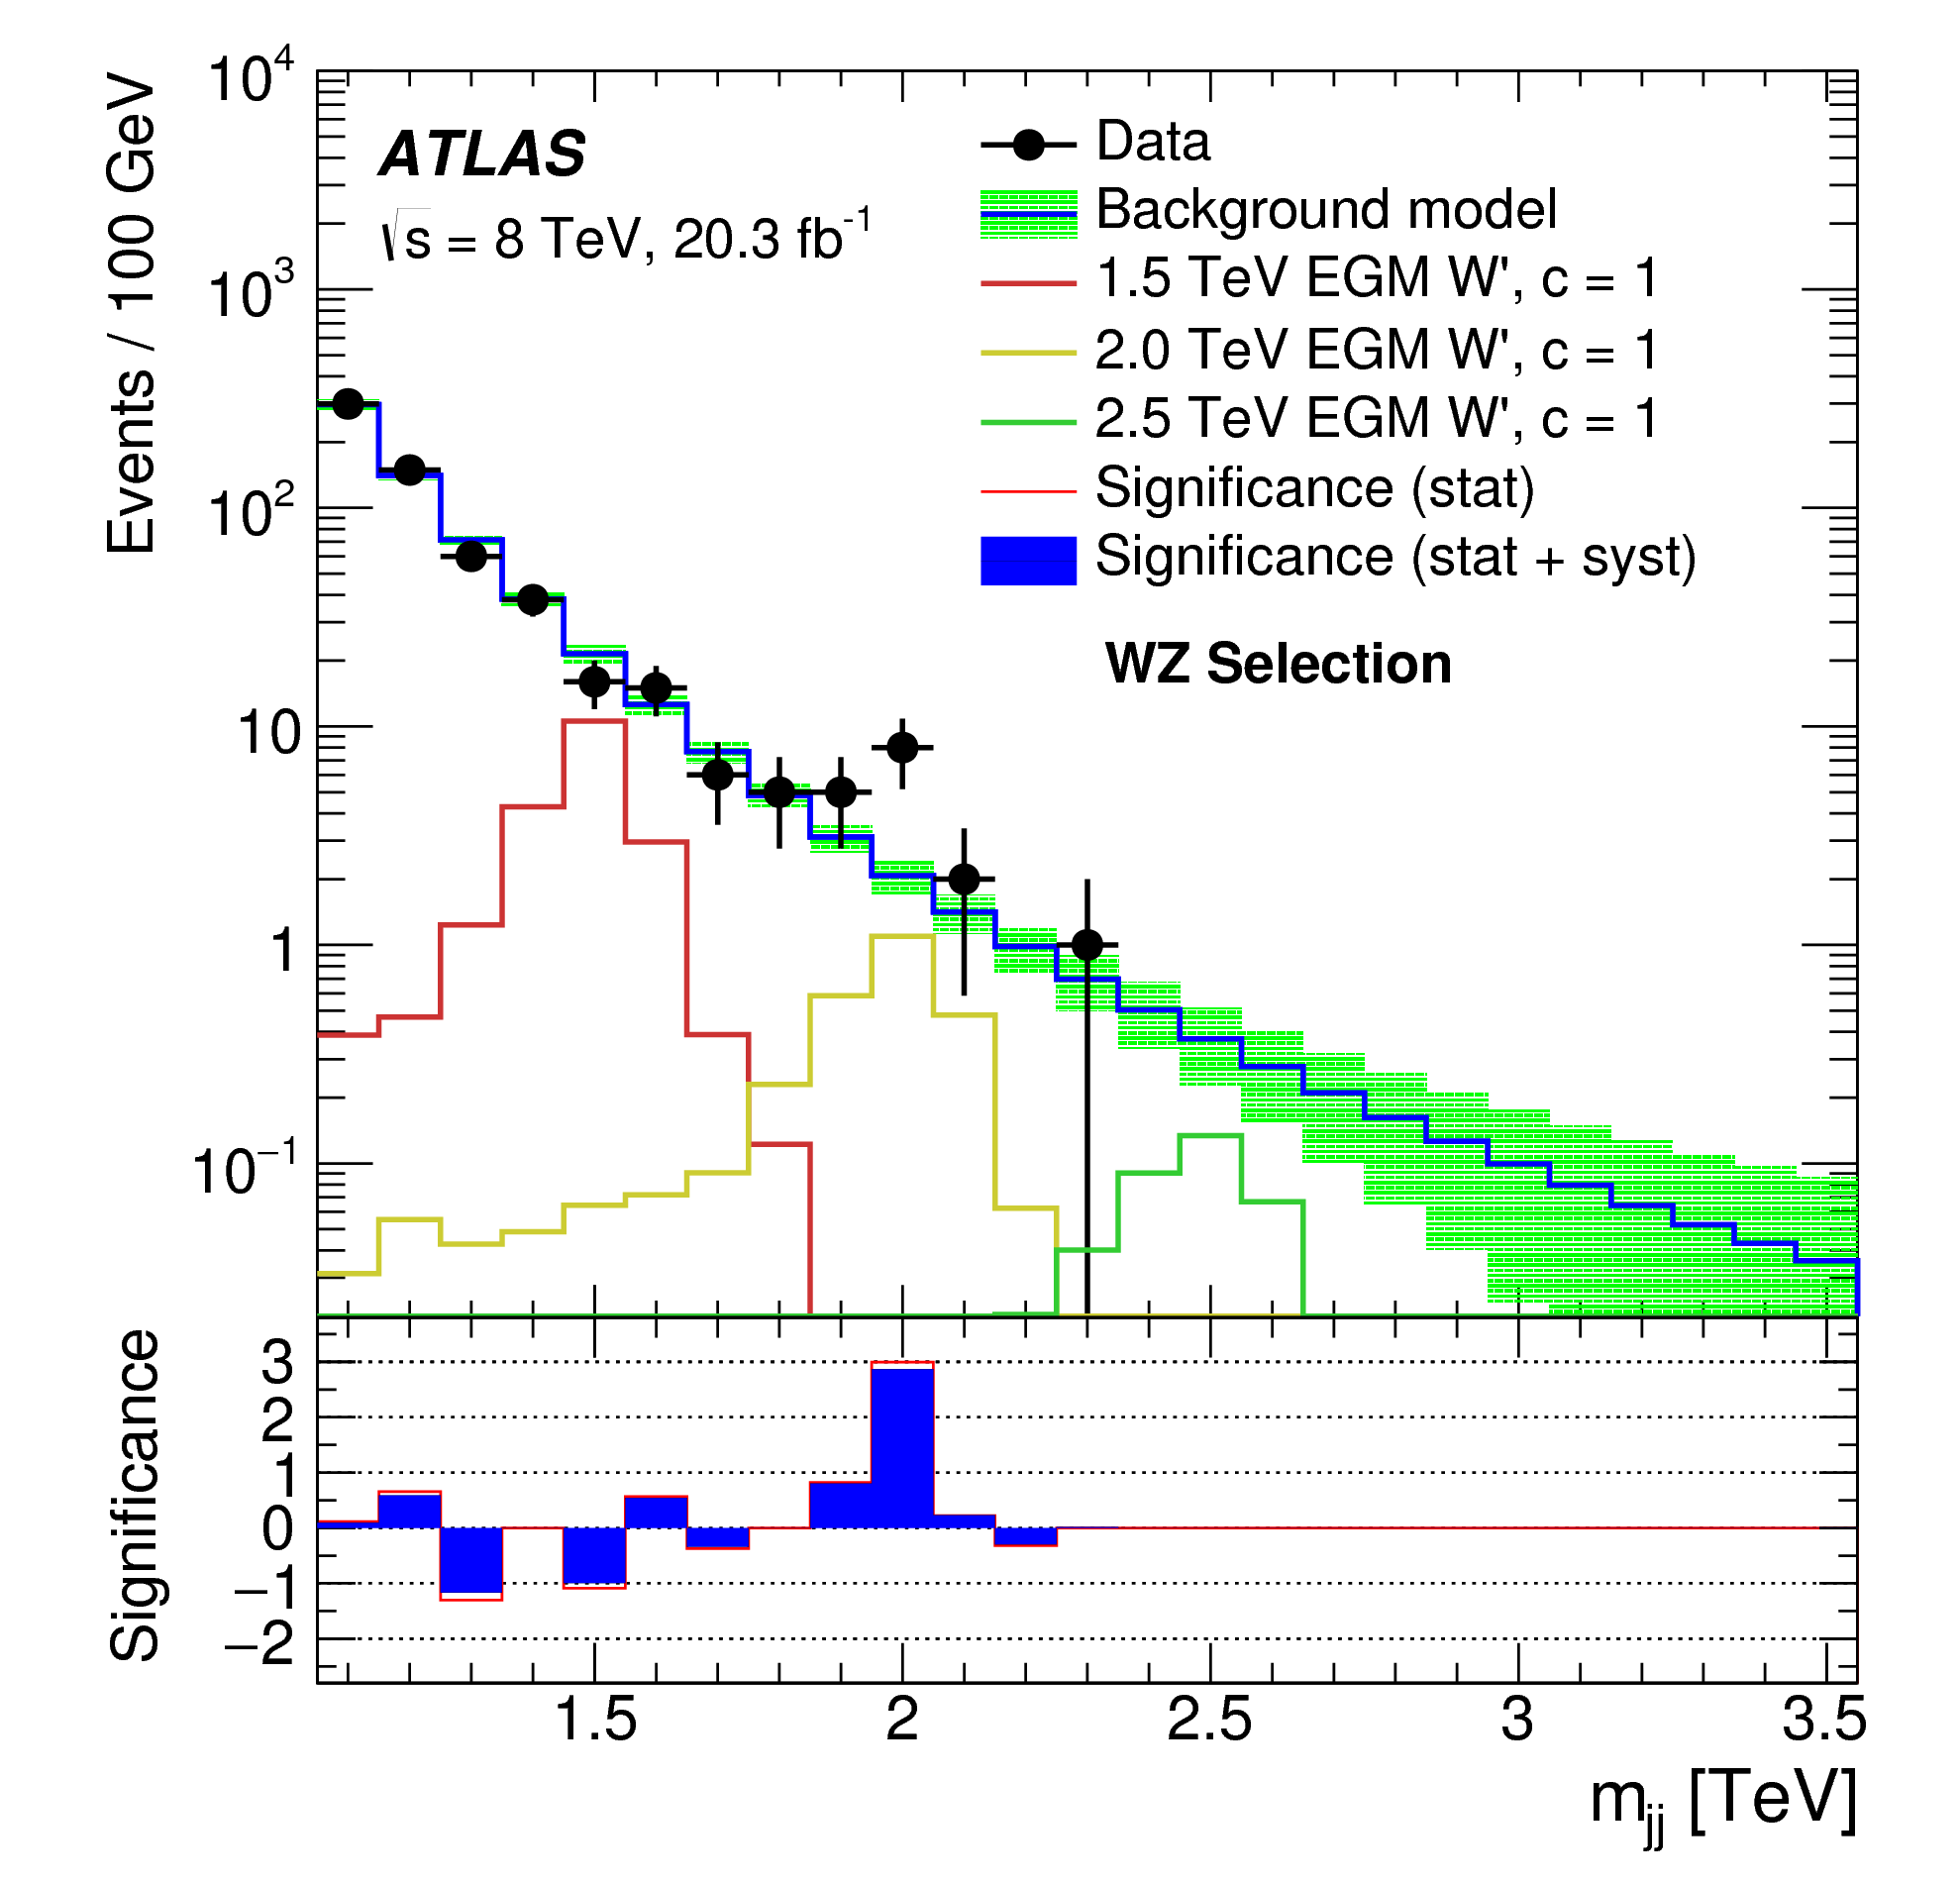
\includegraphics[height=0.3\textwidth]{figures/analysis/search1/misc/atlas_8tev.png}
    %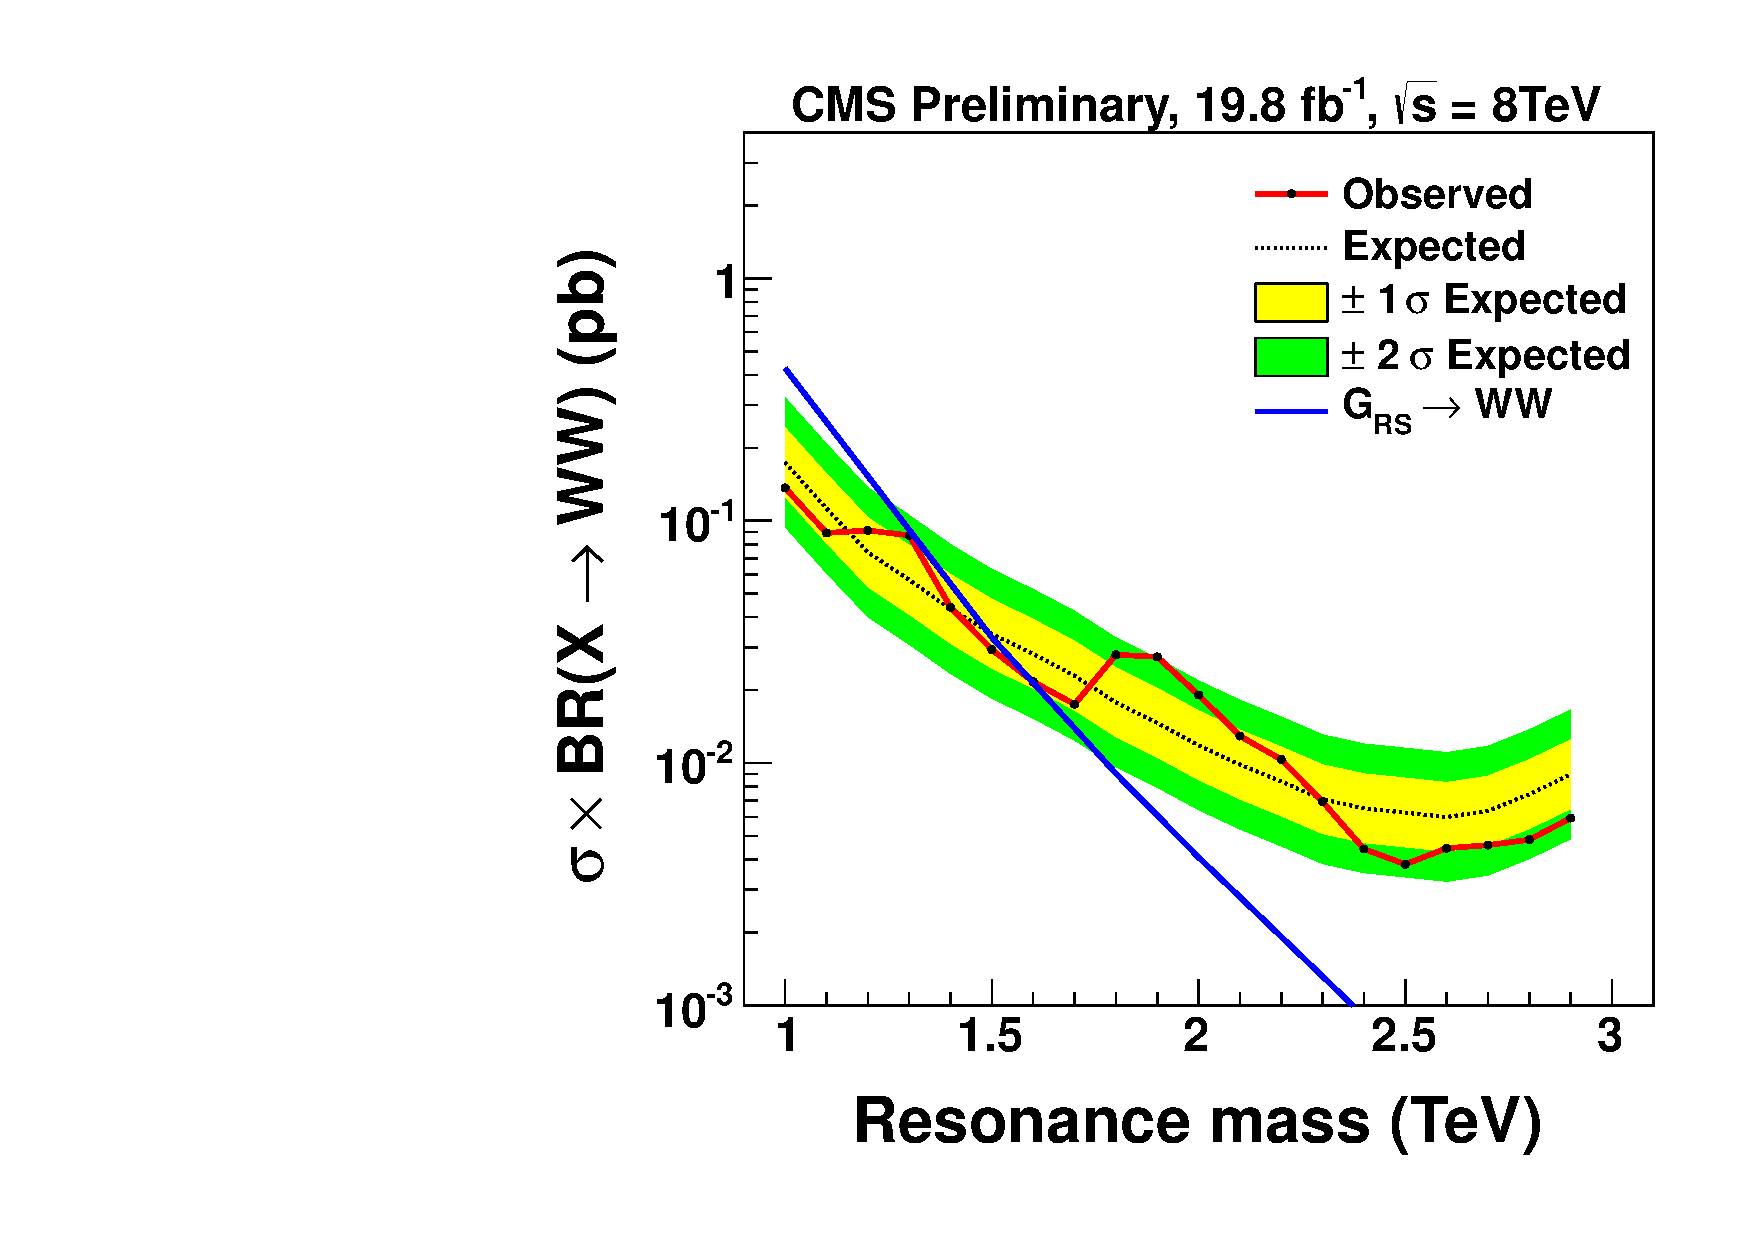
\includegraphics[height=0.3\textwidth]{figures/analysis/search1/misc/EXO-12-024_gWW.pdf}\\
    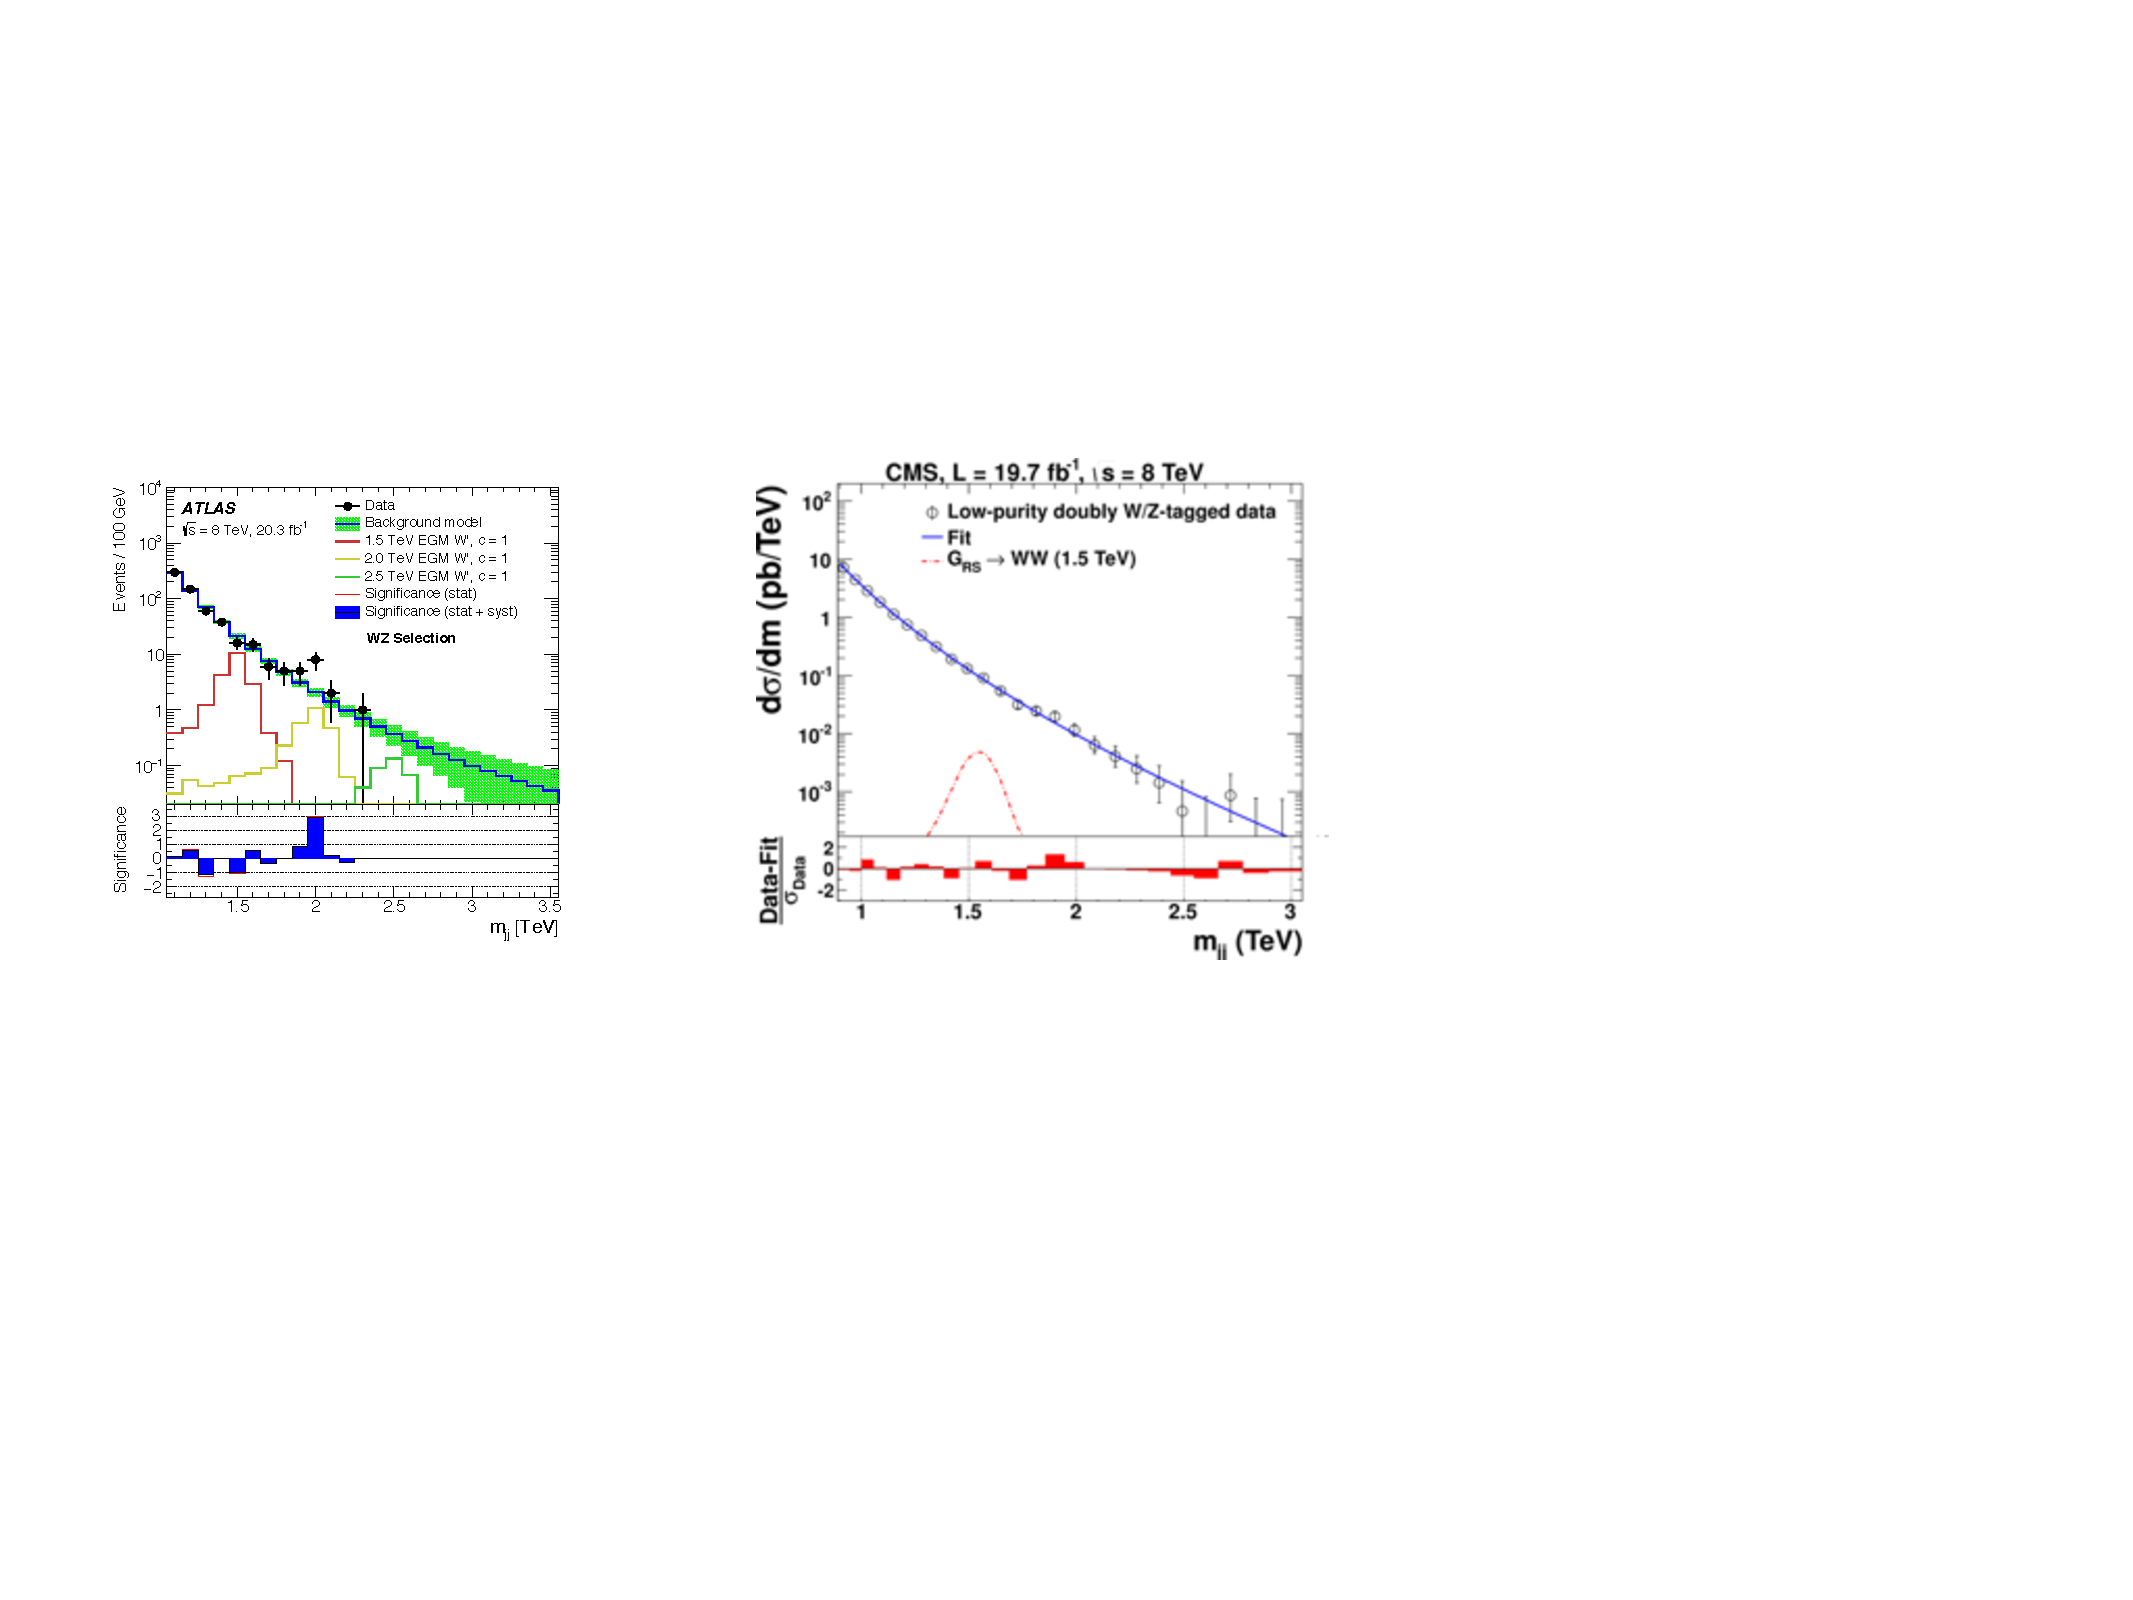
\includegraphics[height=0.2\textwidth]{figures/analysis/search3/misc/bumps2.pdf}\\
    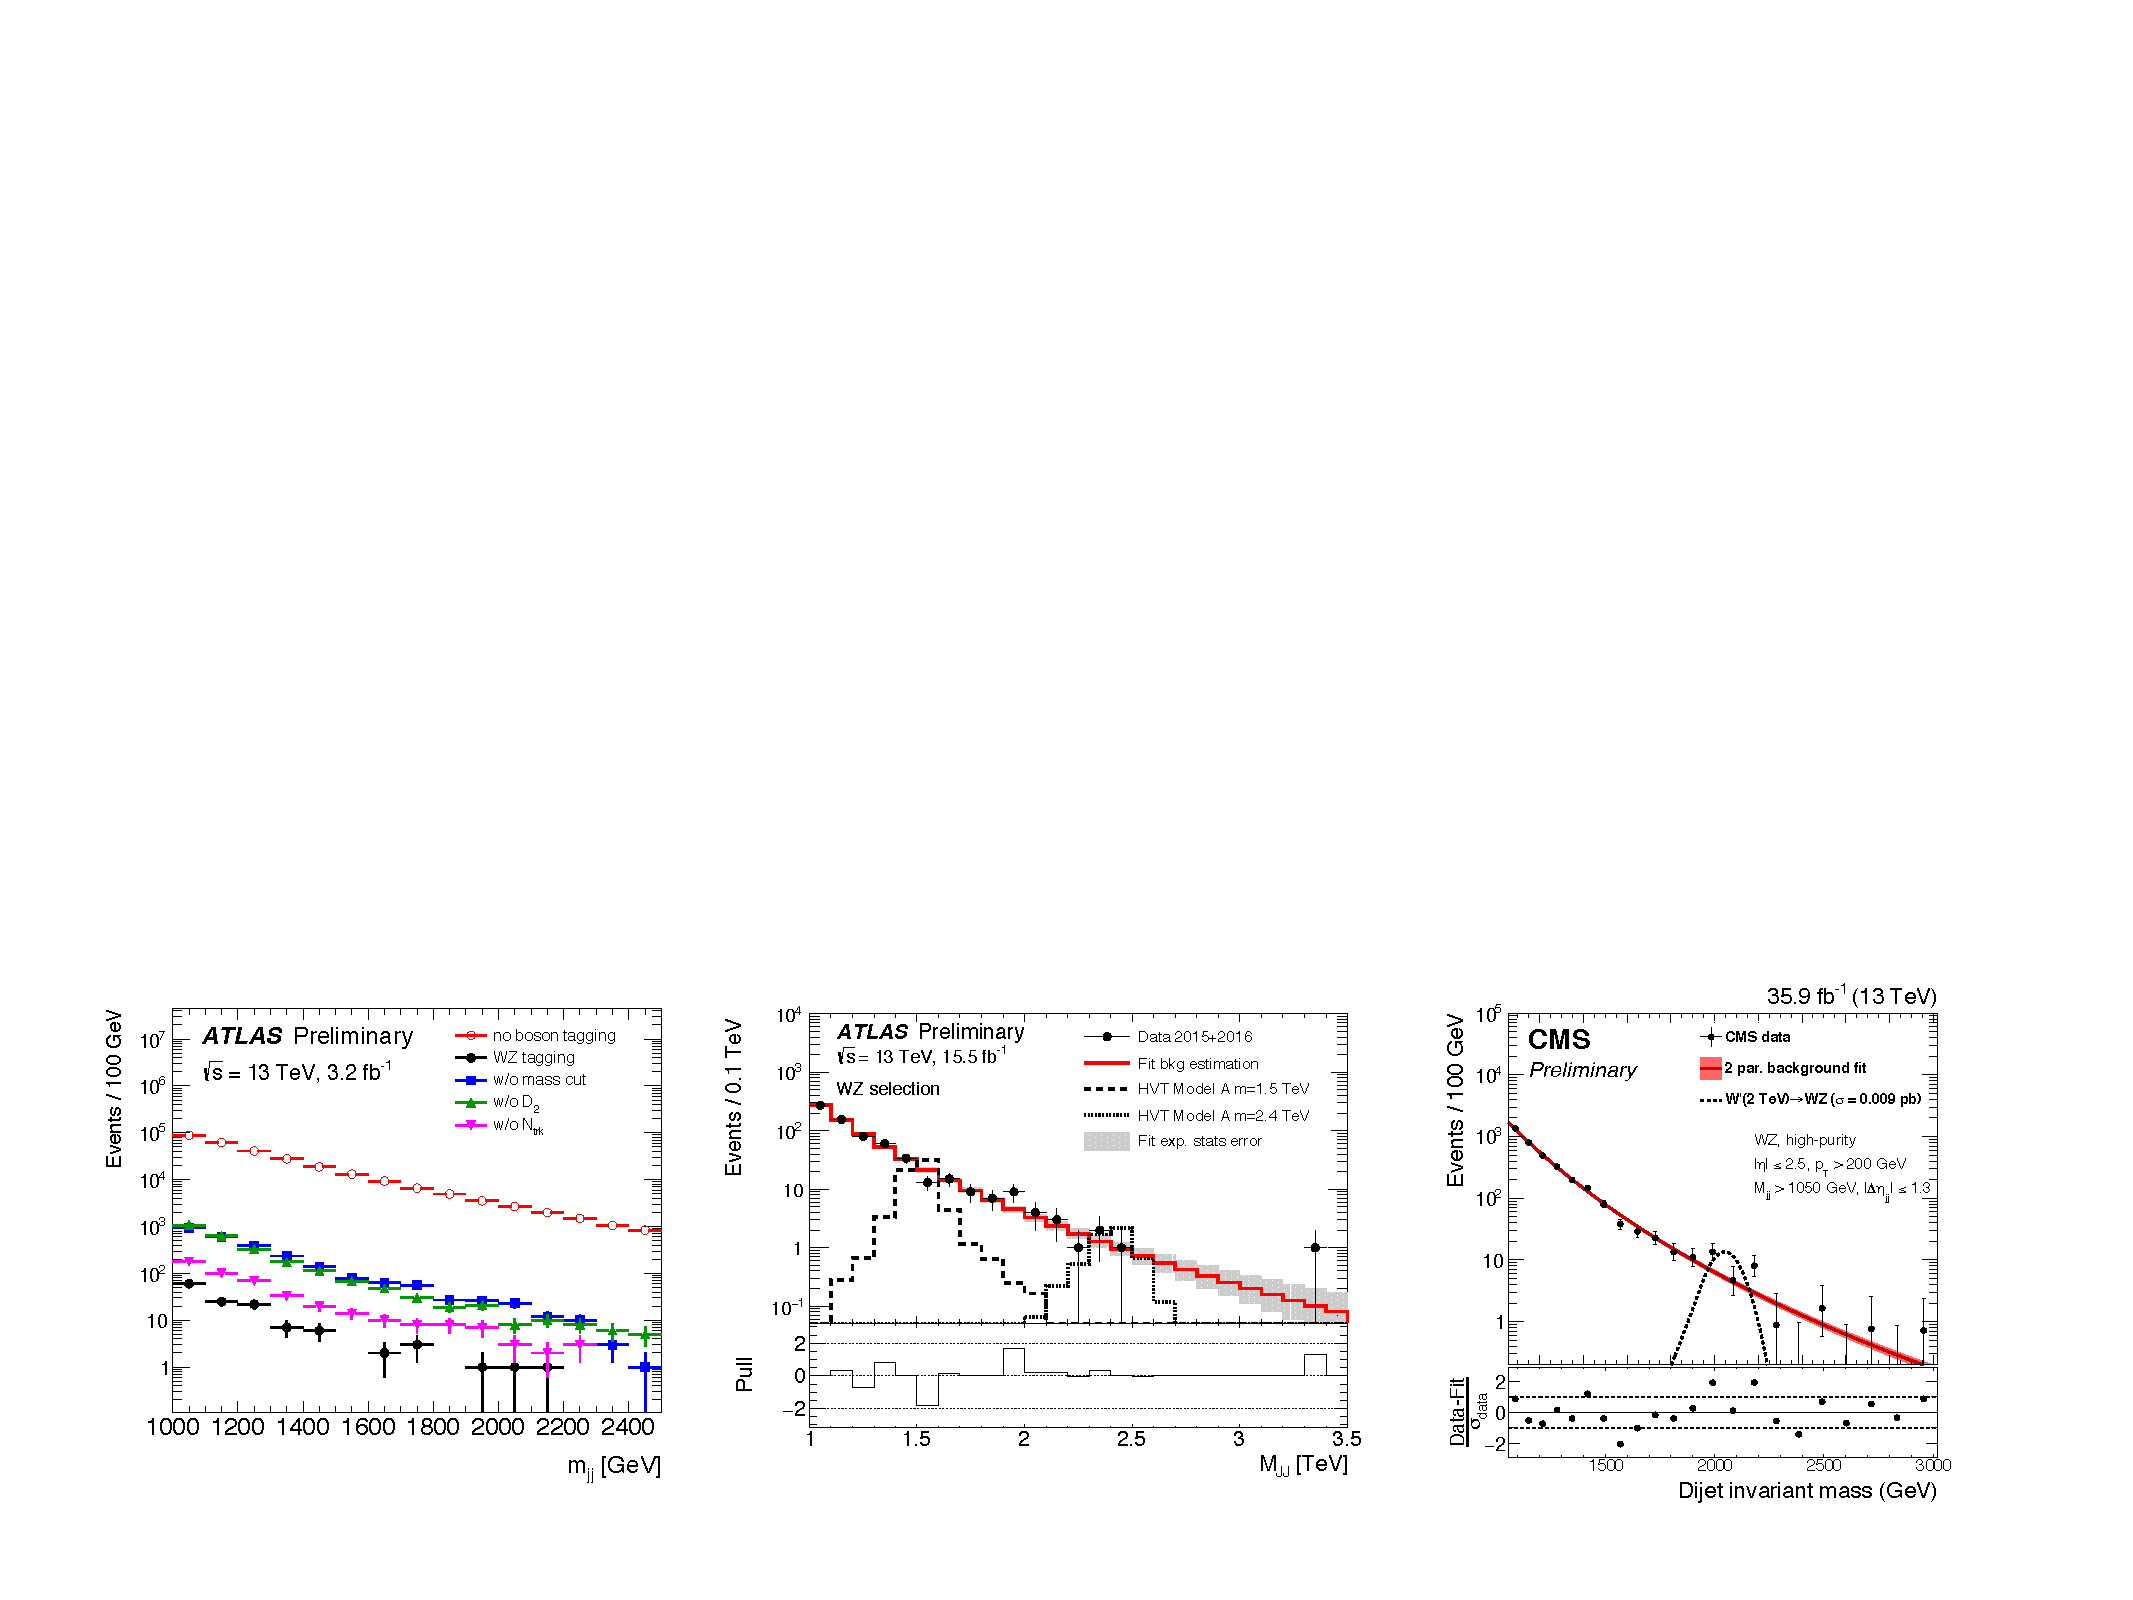
\includegraphics[height=0.2\textwidth]{figures/analysis/search3/misc/bumps1.pdf}\\
    \caption{Several small bumps observed in VV resonance searches in the all-hadronic final state, both in ATLAS and in CMS~\cite{stealth}.}
    \label{fig:searchIII:bumps}
\end{figure}
Due to their small size and the way the excesses seemed to slightly shift around, these were obviously not diboson resonances. However, could they be caused by us catching the tails of some non-SM boson with a mass slightly different from that of a SM vector boson, as illustrated in Figure~\ref{fig:searchIII:tails}?
\begin{figure}[ht] 
    \centering
    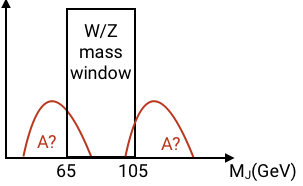
\includegraphics[width=0.3\textwidth]{figures/analysis/search3/misc/tails.png}
    \caption{Slight excesses in diboson analyses could be caused by catching the tail of a non-SM object peaking at slightly higher/lower jet mass than at the W/Z mass.}
    \label{fig:searchIII:tails}
\end{figure}
Further, these could be 4-pronged objects rather than 2-prong, which would cause the excess to vary in size depending on the 4-prong efficiency of the analysis specific W-tagger used.\newline
An explanation for the observed excesses was proposed in~\cite{Aguilar-Saavedra:2018xpl}. This paper pointed out that, if particles like \PWpr and \PZpr exist, an extended scalar sector is needed in order to give mass to the
vector bosons. These heavy scalars will decay to lighter bosons, if kinematically allowed, leading to multiboson signals from cascade decays. Some example signatures are illustrated in Figure~\ref{fig:searchIII:tribosons}.
\begin{figure}[ht] 
    \centering
    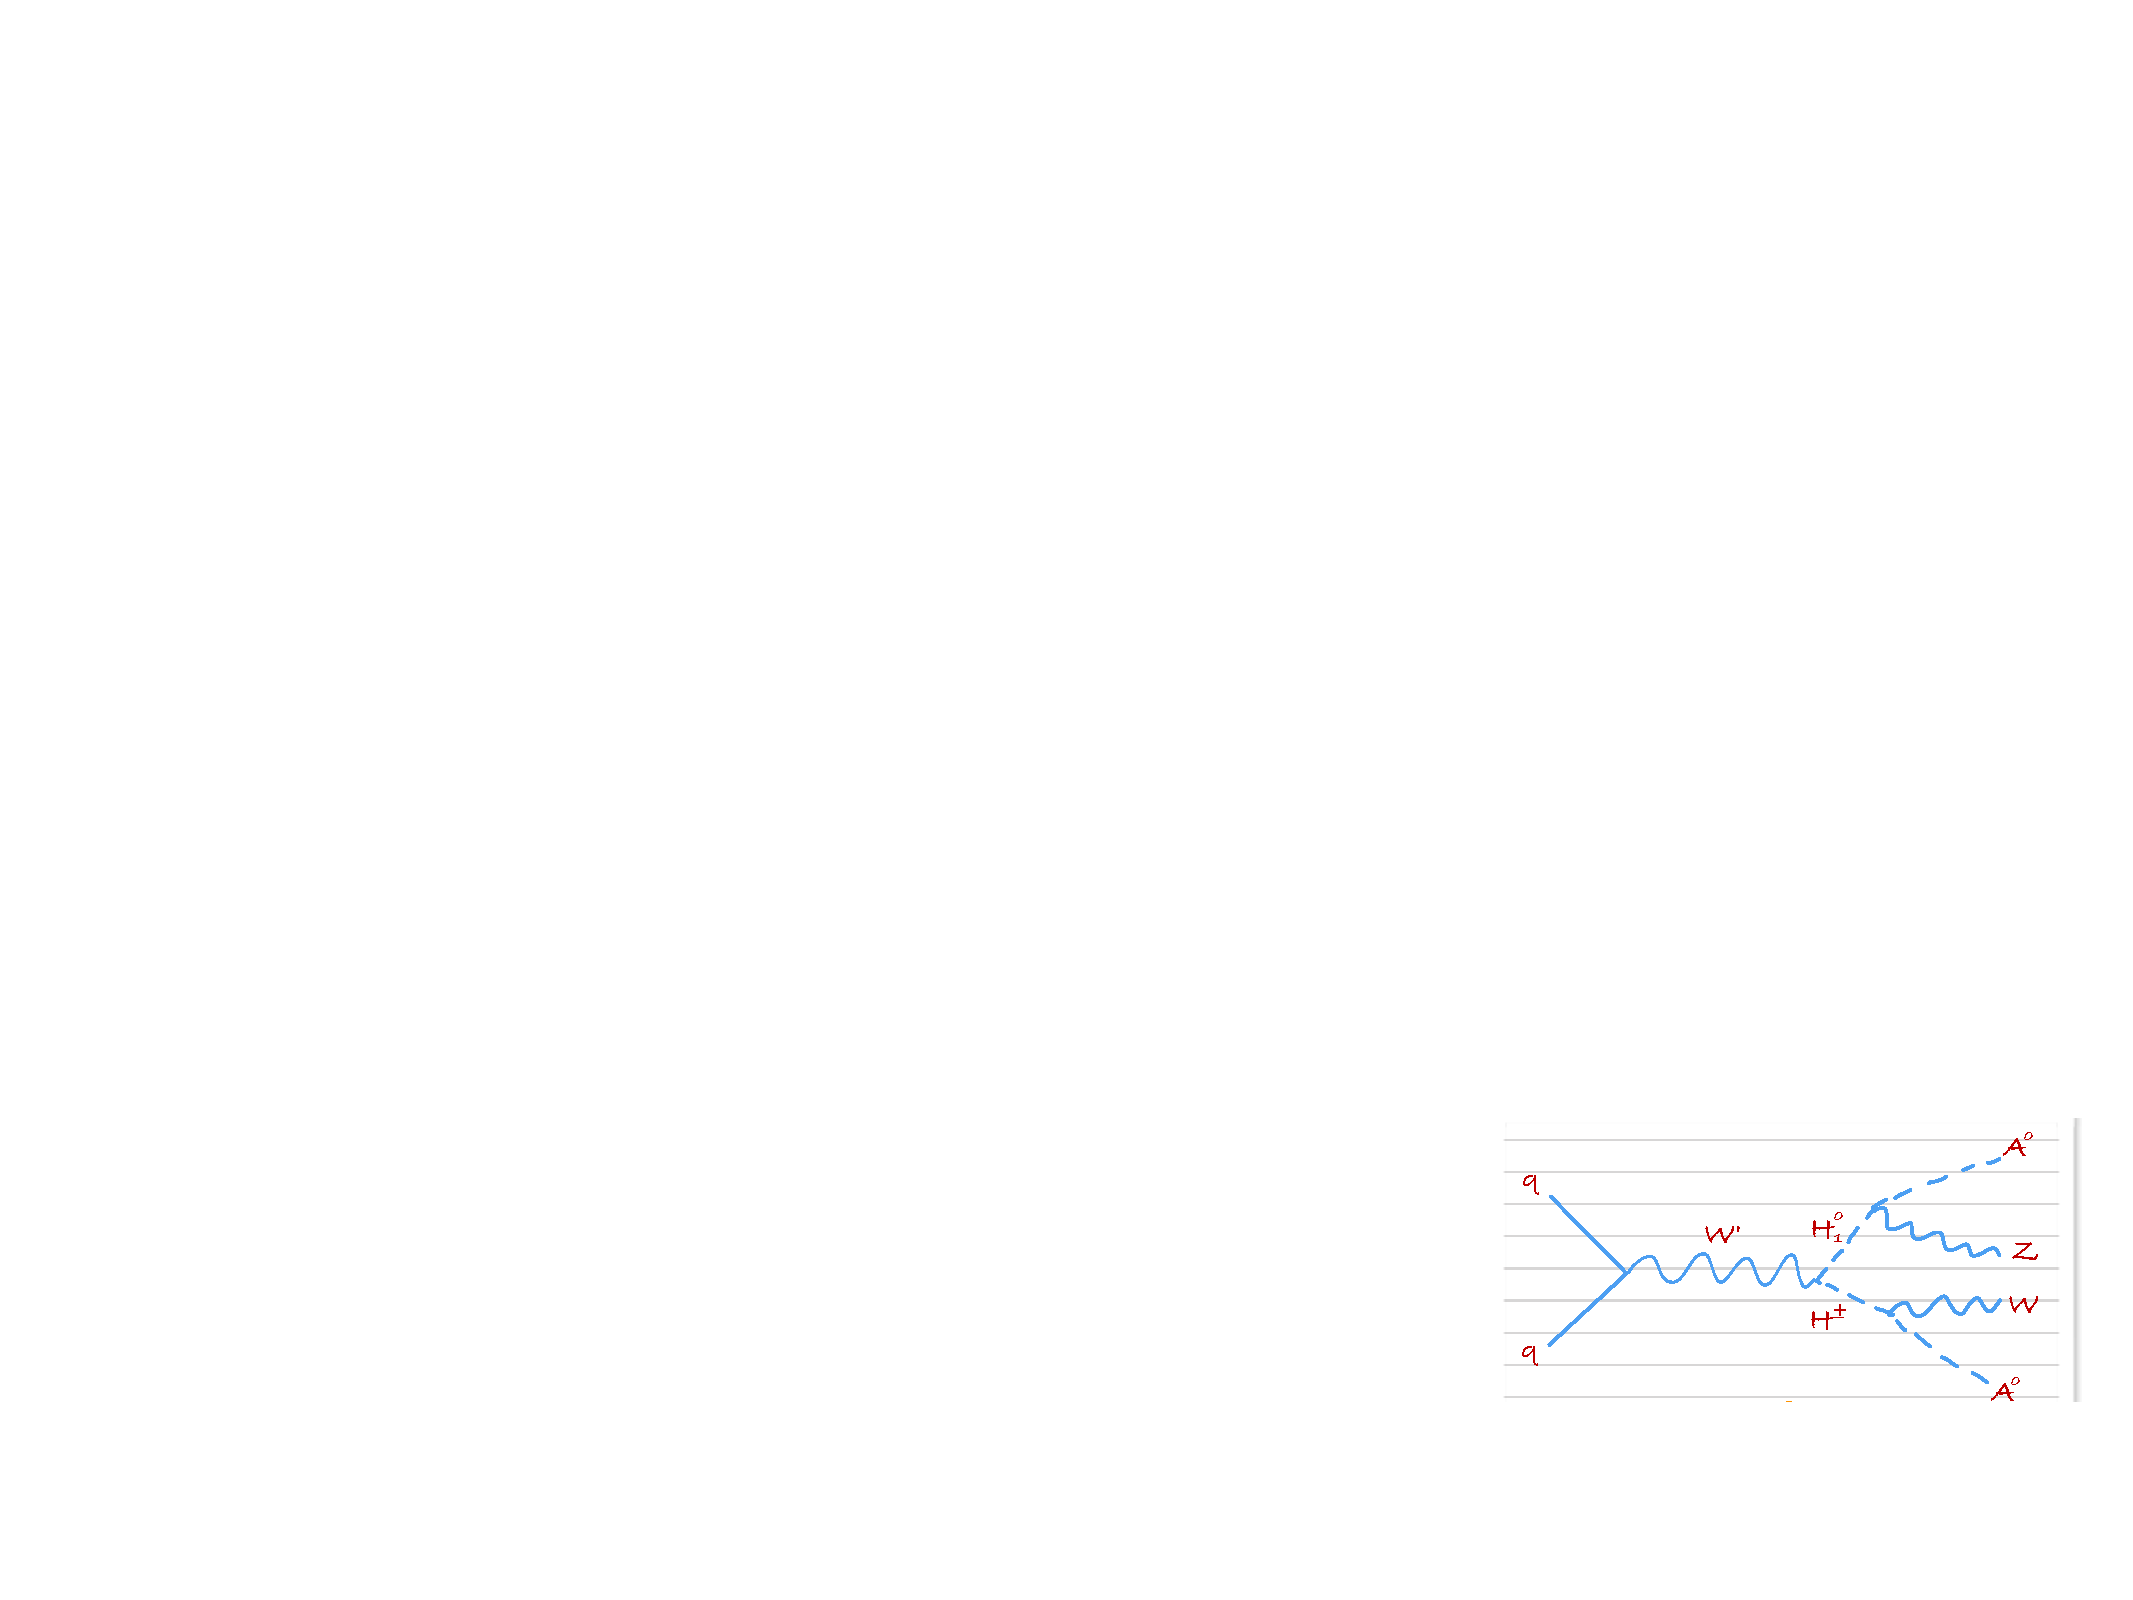
\includegraphics[height=2cm]{figures/analysis/search3/misc/quadri.pdf}
    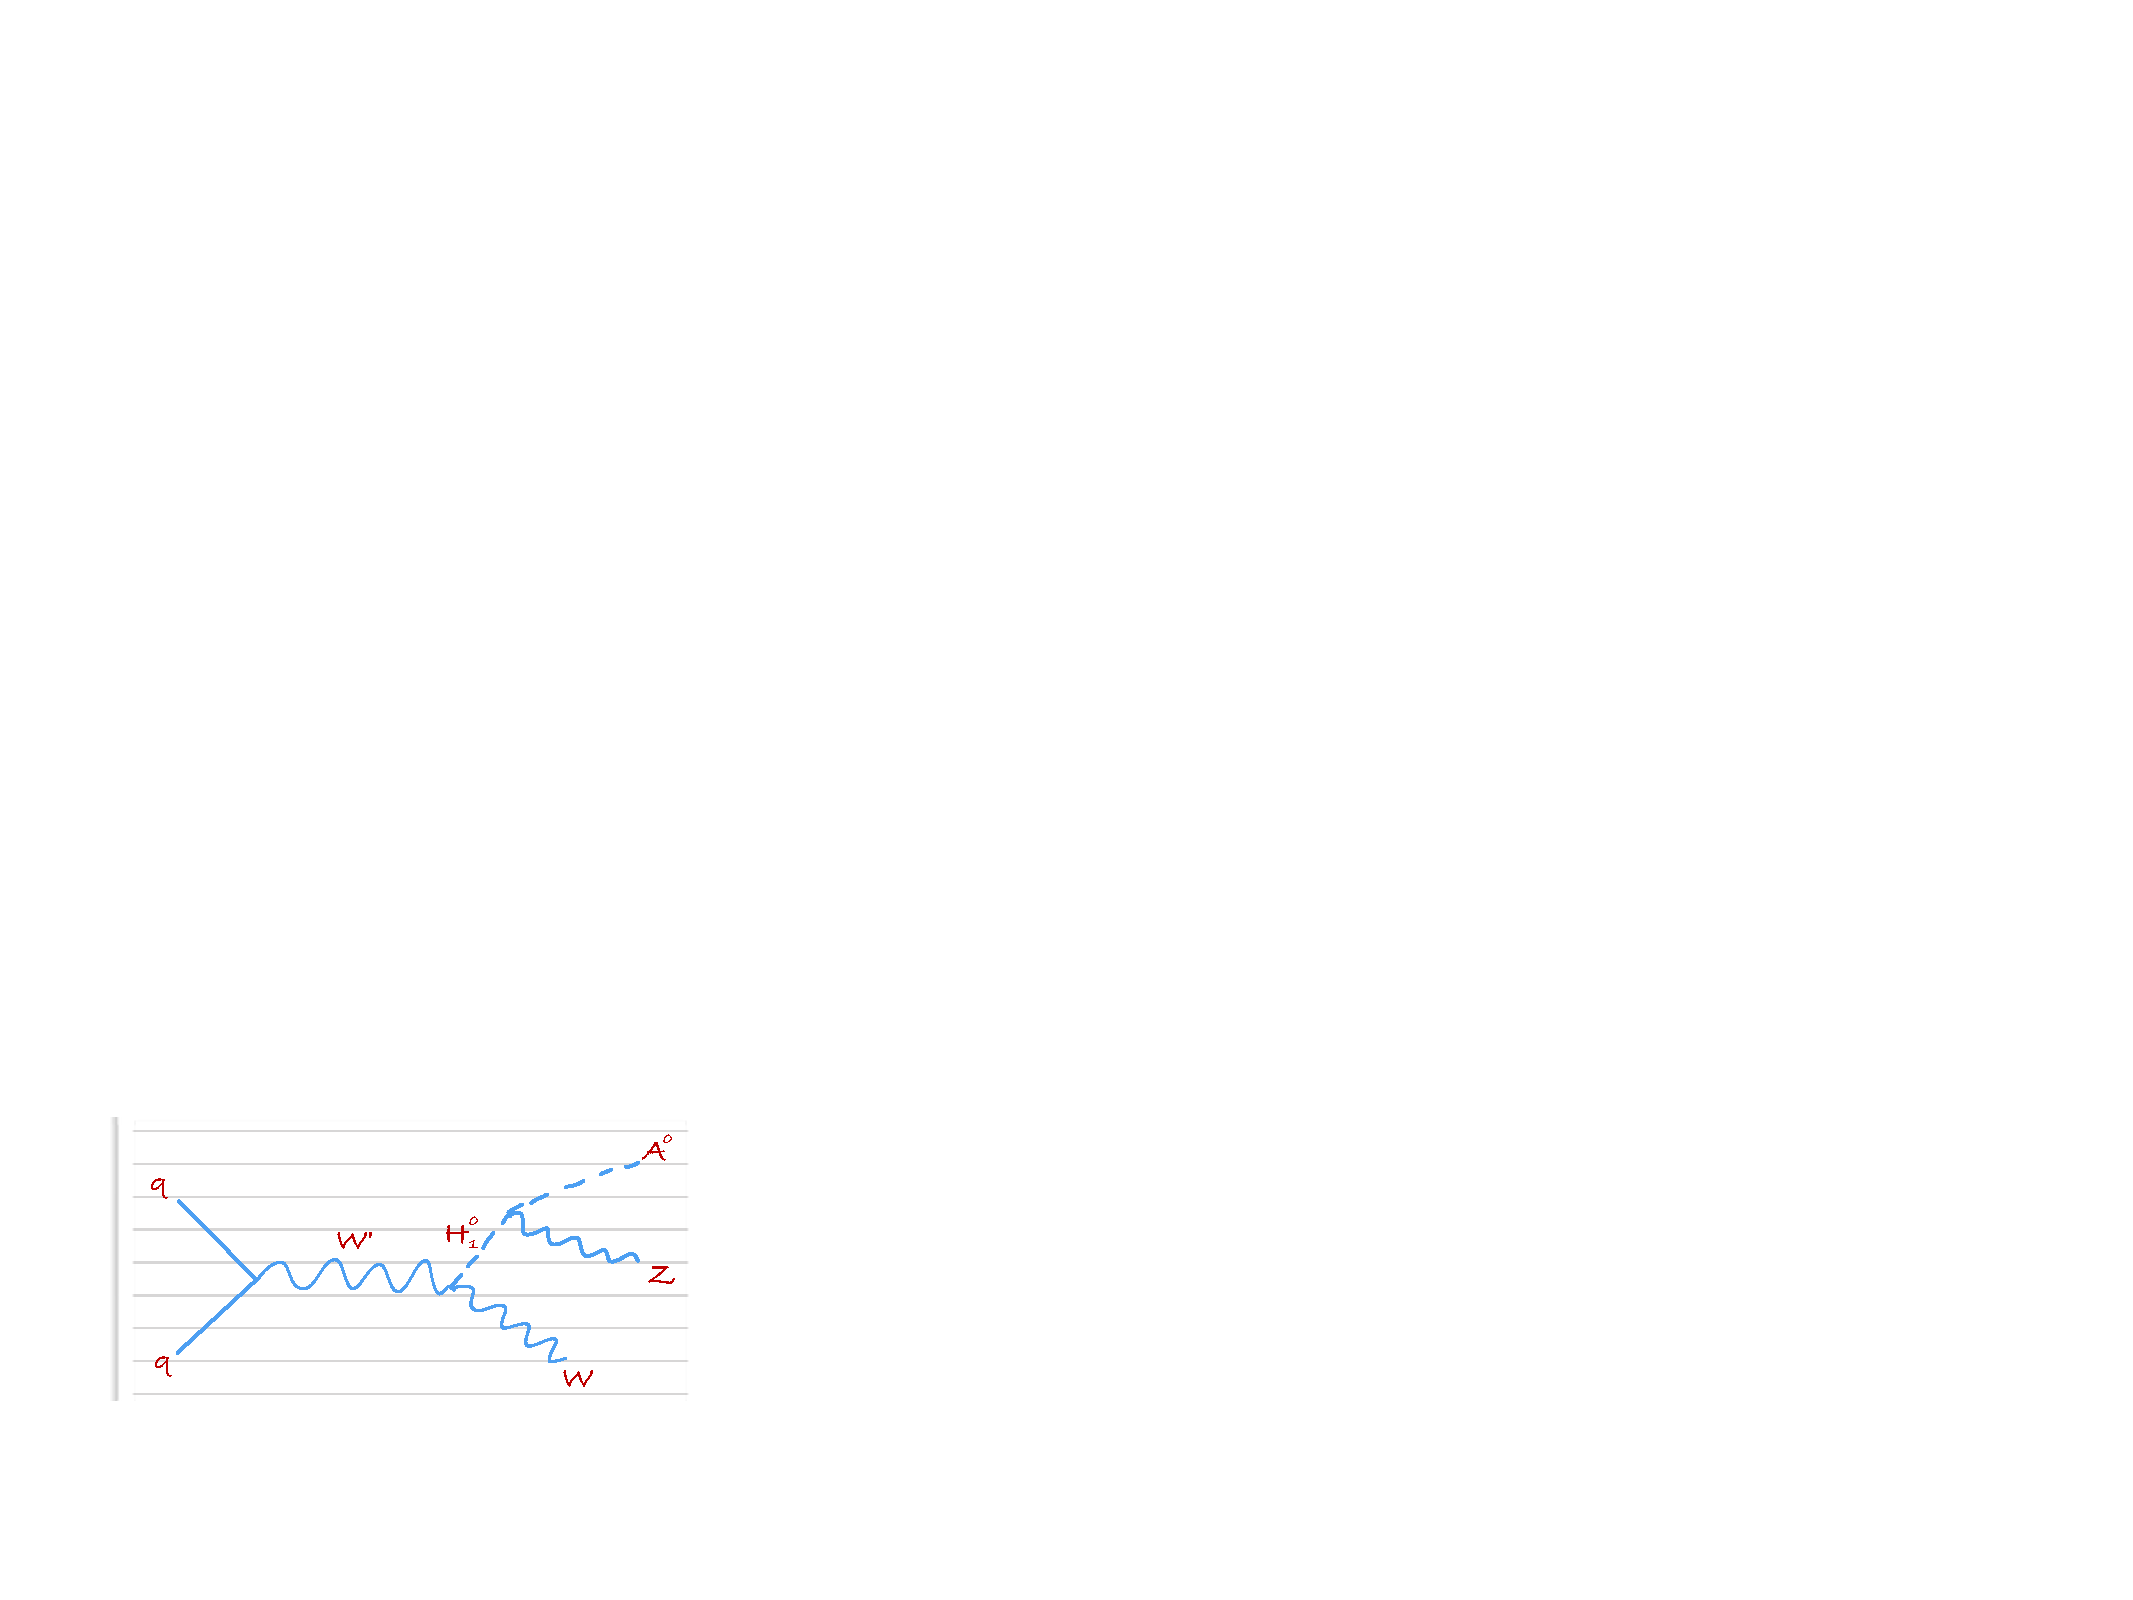
\includegraphics[height=2cm]{figures/analysis/search3/misc/tri1.pdf}
    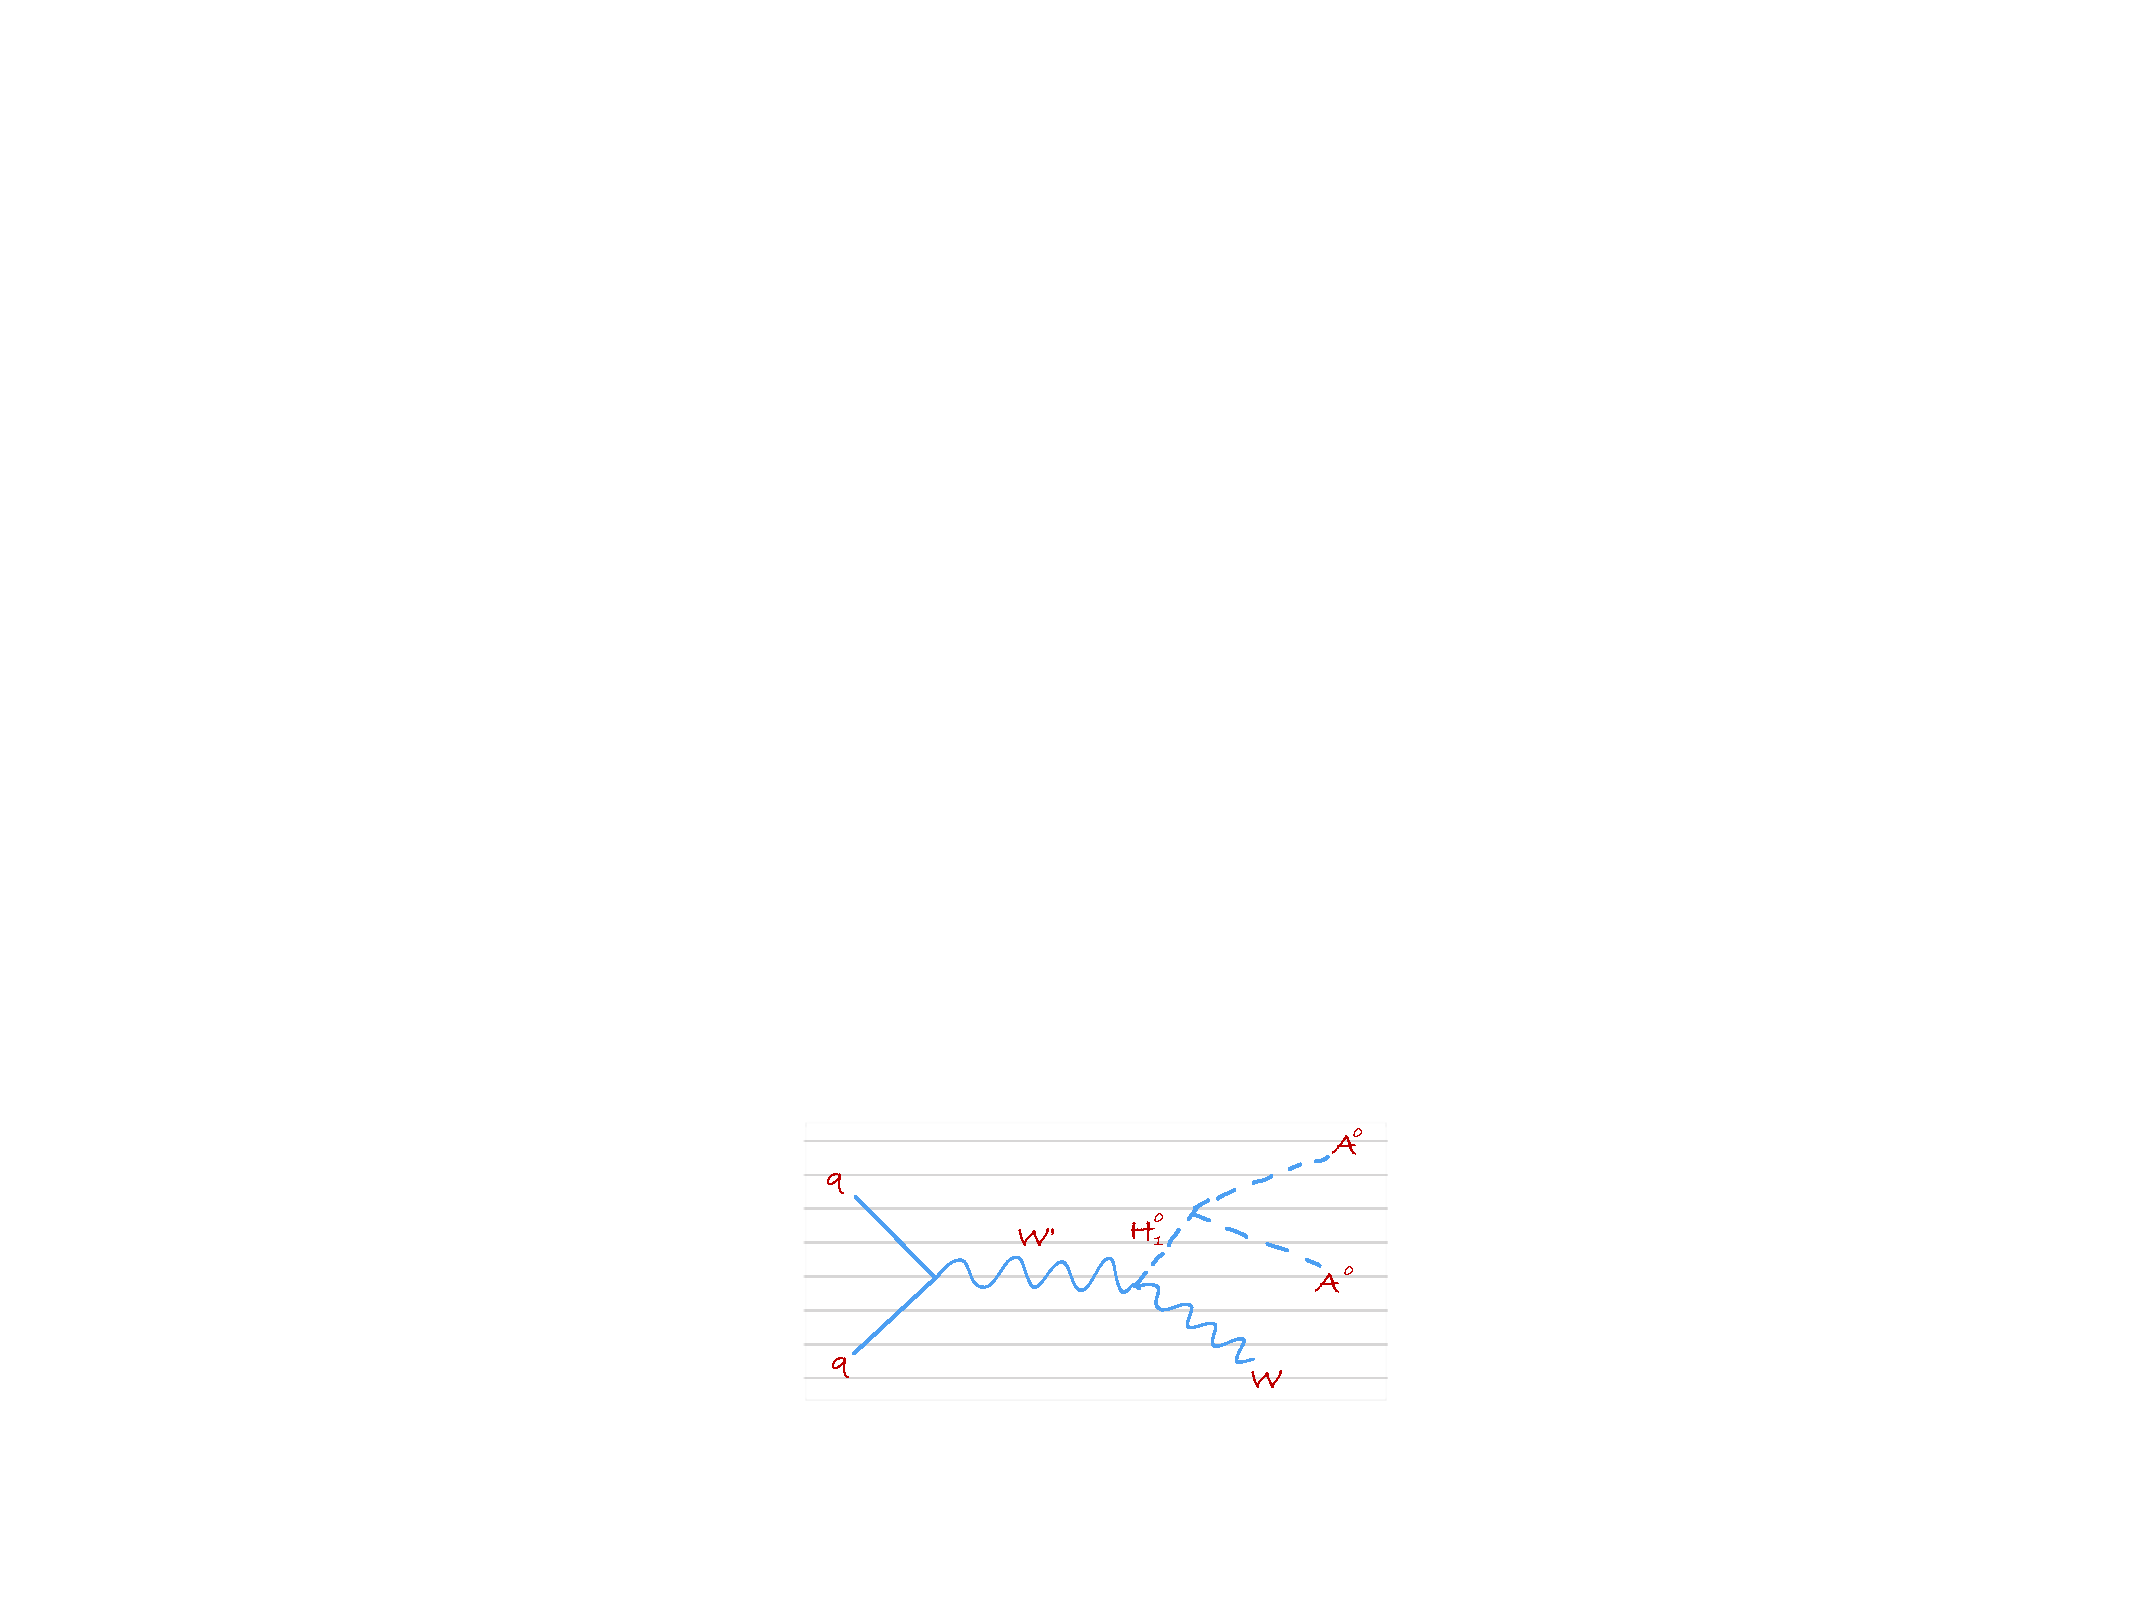
\includegraphics[height=2cm]{figures/analysis/search3/misc/tri2.pdf}
    \caption{A \PWpr decaying to a neutral $\rm{H}^0$ and a charged $\rm{H}^{\pm}$ scalar particle leading to a quadriboson final state (left), and a \PWpr decaying to a neutral scalar particle $\rm{H}^0$ and a \PW leading to a triboson final state (middle and right)~\cite{Aguilar-Saavedra:2018xpl}.}
    \label{fig:searchIII:tribosons}
\end{figure}
Signatures like these would peak in the groomed jet mass spectrum and, depending on what the final bosons decay into, have very different substructure profiles (4- and 4-prong, 2- and 4-prong etc.).\par
In order to effectively search for such types of signals, or any signal peaking in the softdrop jet mass spectrum, we therefore wanted to build a generic new framework allowing to look for peaks anywhere in the groomed mass - dijet invariant mass spectrum.
Rather than selecting jets with a groomed mass between 65 and 105 \GeV and look for resonances peaking in the dijet invariant mass, we'd look for resonances peaking anywhere in the three dimensional plane formed by the groomed mass of each jet and their invariant mass.
The benefits of this procedure, was that it would allow us to scan the full groomed mass spectrum in one analysis. We would first demonstrate the method through the VV all-hadronic analysis, which is the paper introduced here.
\subsection{Analysis strategy}
The background estimation used in Search I and Search II rely on a one dimensional fit of the dijet invariant mass signal region after a tight jet mass cut (65-105 \GeV) has been applied.
We now take advantage of the fact that the signal peaks in three dimensions; dijet invariant mass ($\MVV$) and the jet groomed mass of jet 1 and jet 2 ($\MJO$ and $\MJT$),
and attempt to extract the signal from the three dimensional $\MVV$-$\MJO$-$\MJT$ plane.
\begin{figure}[h!] 
    \centering
    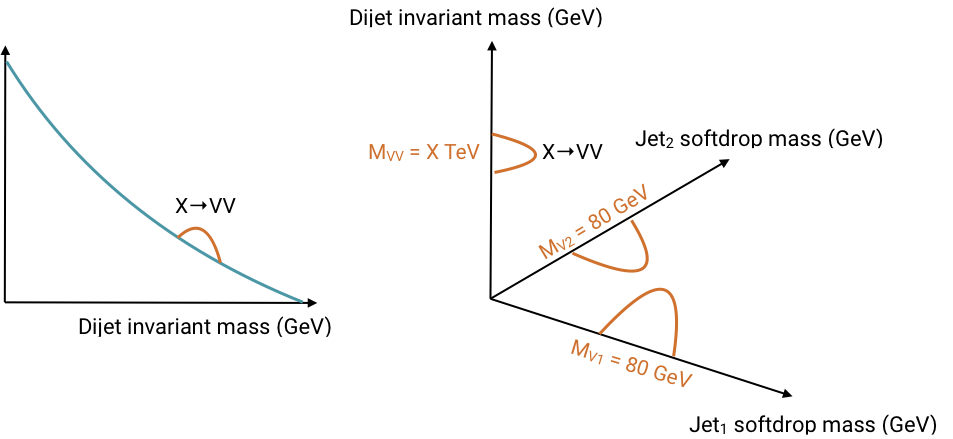
\includegraphics[width=0.79\textwidth]{figures/analysis/search3/misc/1Dvs3D.png}
    \caption{The one dimensional VV analysis versus the three dimensional fit.}
    \label{fig:searchIII:1Dvs3D}
\end{figure}
The benefits of doing so is that we now can perform different searches in the $WW, WZ, ZZ, WH$ or $XX$ final states encoded in the same analysis.
Additionally, tight jet mass cuts are no longer needed as we fit the full jet mass line-shape to extract the signal. This effectively increases our signal statistics
as a large fraction of the $W$ and $Z$ signal fall outside the above mass window.
Fitting the jet groomed mass and resonance mass together also allow us to add nuisance parameters that simultaneously affect the jet groomed mass and the resonance mass, fully accounting for the correlation between the variables.
We would model the background starting from simulation, rather than the dijet fit to data, which would allow us to model peaky distributions like a trigger turn-on. This could allow the search to go even lower in \MVV, something we will discuss further in Section~\ref{sec:searchIII:trigger}. \newline
This chapter, and its corresponding publication, is an analysis of the 2016 and 2017 dataset, corresponding to $\sim 80 \fbinv$, and serves as the first documentation and demonstration of the novel three-dimensional fit method. In Section~\ref{sec:outlook}, I'll discuss how we plan to take this framework further in searches for VH and HH as well as for generic resonances peaking in jet softdrop mass.
\subsection{Data and simulated samples}
The data analyzed in this search consists of 35.9 \fbinv of data collected in 2016 ands 41.4 \fbinv of data collected in 2017, yielding a total of 77.3 \fbinv.\newline
The simulated samples are the same as those described in Section~\ref{sec:searchII:samples}, with specific detector conditions to match the 2016 and 2017 dataset.

\subsection{Event selection}
Events are selected following the same criteria as in Search I and Search II (see Section~\ref{sec:searchI:preselection}) and can be summarized as follows:
\begin{itemize}
    \itemsep0em 
\item PF jet Tight ID applied
\item Jet $\eta < 2.5$
\item Jet \pt $> 200$ GeV
\item $|\Delta\eta|_{jj} < 1.3$
\end{itemize} 
The two jets with the highest groomed jet mass in the event are selected as potential vector boson candidates. In addition, the dijet invariant mass is required to be $> 1126$ GeV in order to be on the trigger plateau.
As already mentioned in the introduction, the background modeling used in this analysis is capable of modeling turn-ons and is something we explored. However, while the background modeling was reliable, we found it difficult to extract a signal peaking on top of a turn-on and had to abandon the trigger modeling for this first demonstration of the method. More details will be given in Section~\ref{sec:searchIII:trigger}.\newline 

The dijet invariant mass and $|\Delta\eta|_{jj}$ distribution for the two leading jets in the event after the above preselections have been applied is shown in Figure~\ref{fig:Mjj-all}. The jet \PT{} and $\eta$ distributions for signal and for background is shown in Figure~\ref{fig:kinematics-all}. 

\begin{figure}[h!]
\centering
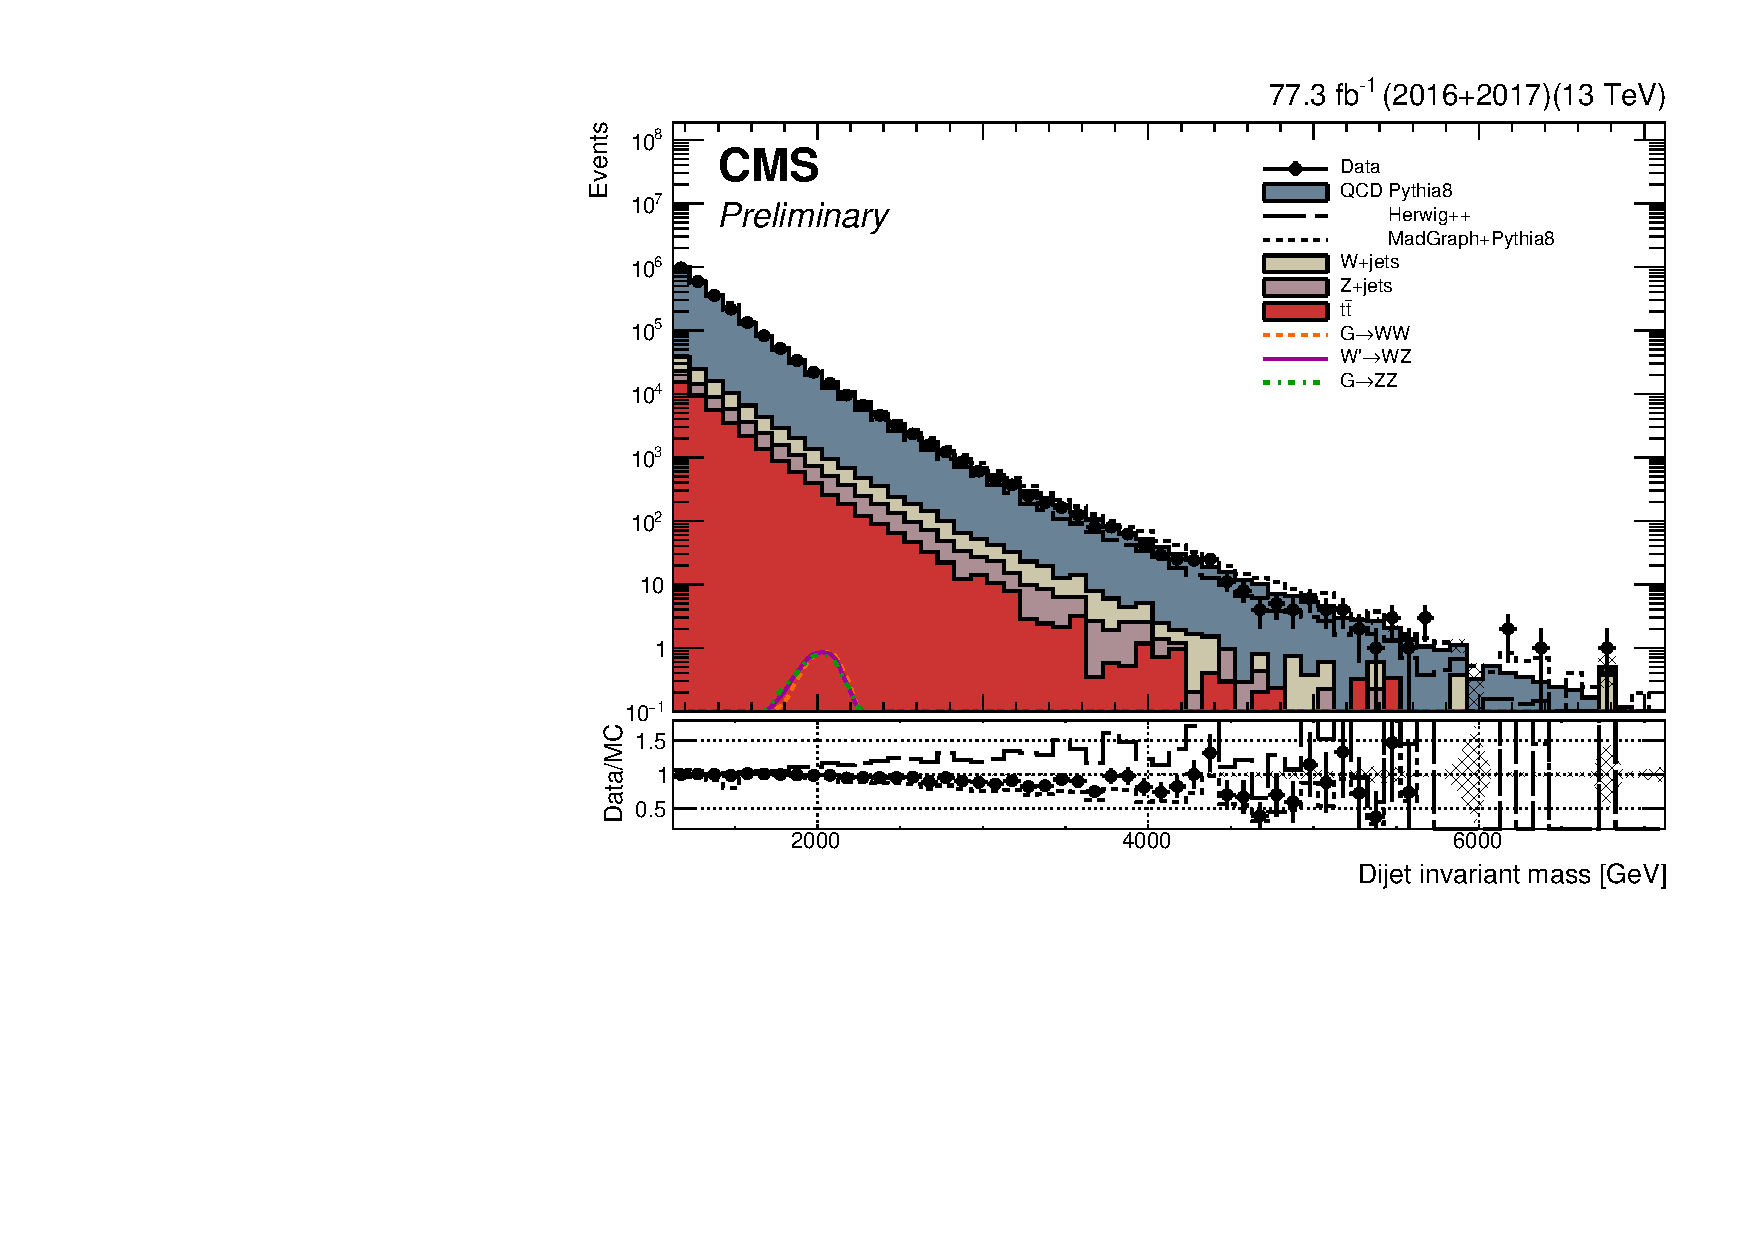
\includegraphics[width=0.450\textwidth]{figures/analysis/search3/AN-17-303/controlPlots/looseSel_Dijet_invariant_mass.pdf}
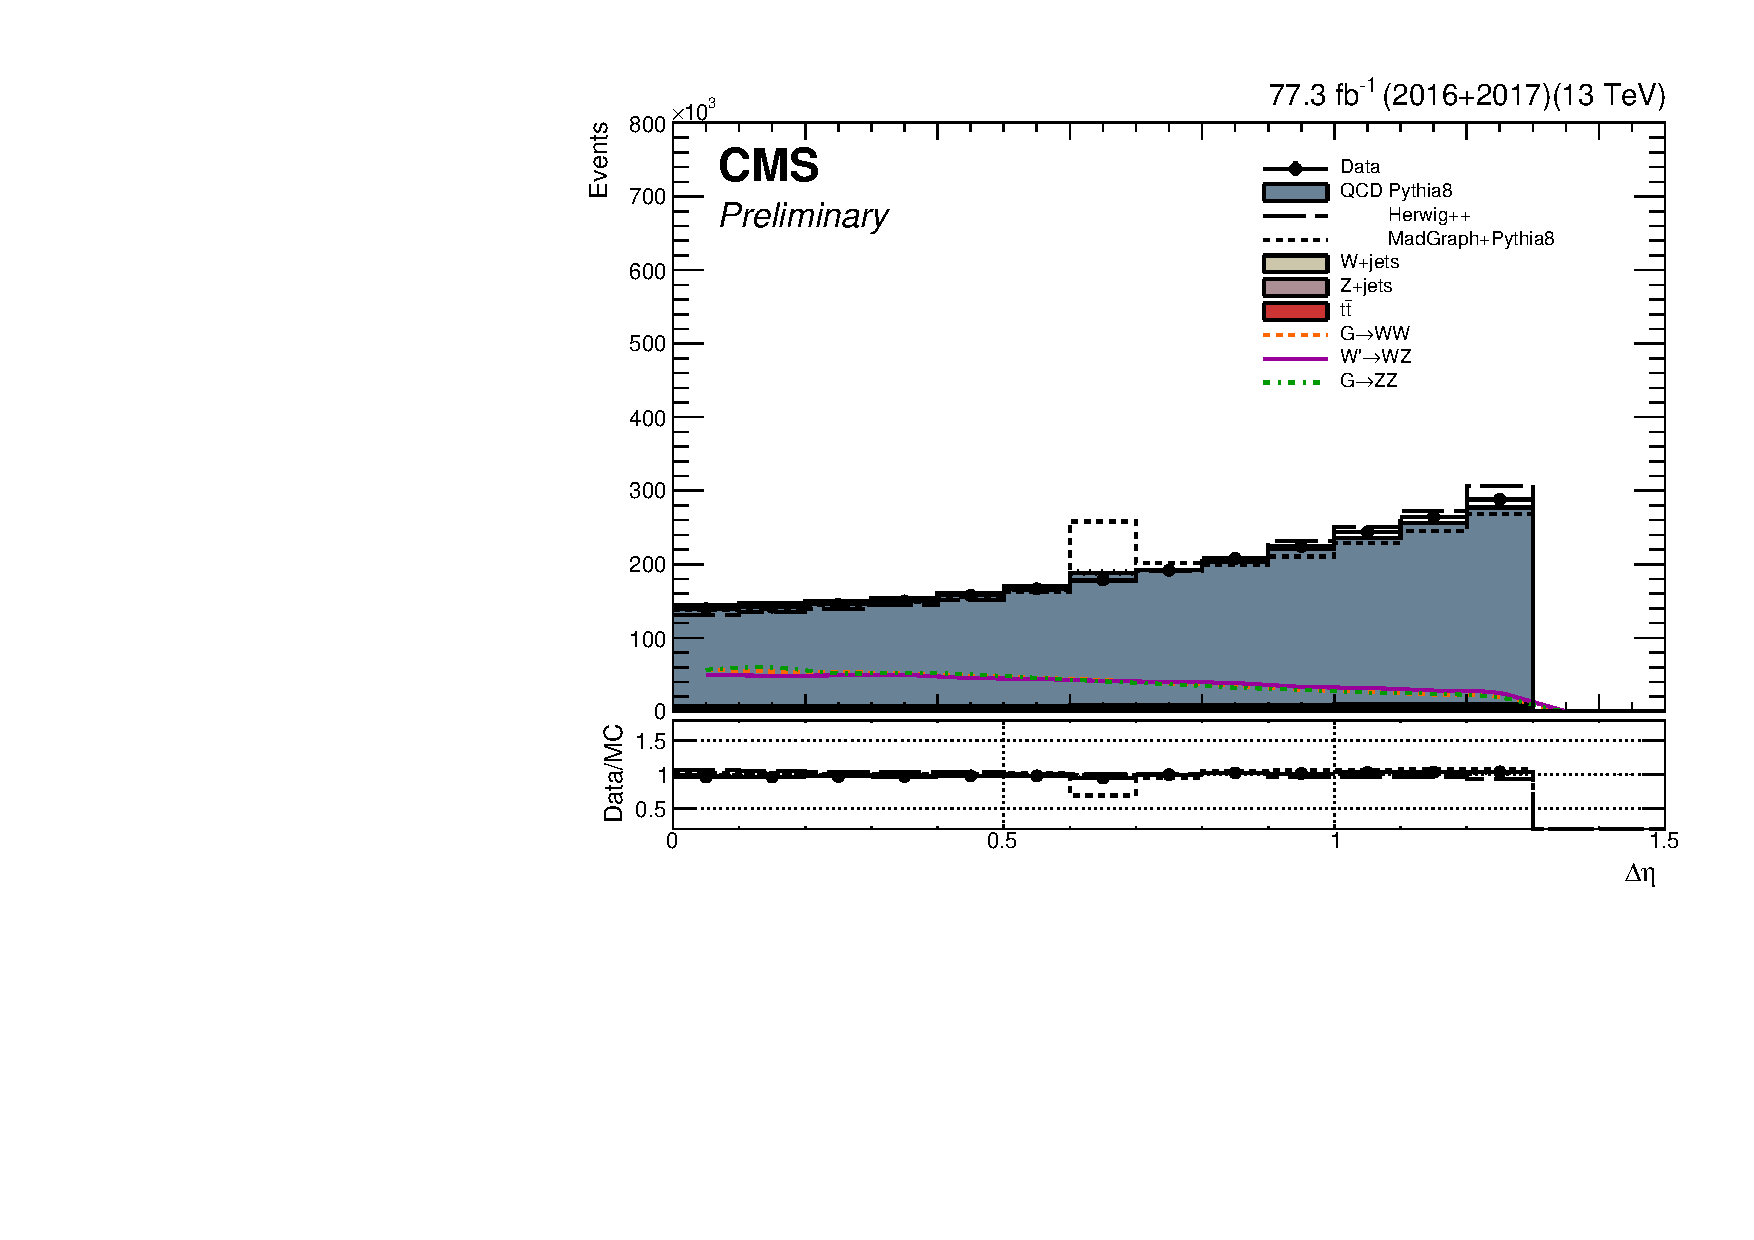
\includegraphics[width=0.450\textwidth]{figures/analysis/search3/AN-17-303/controlPlots/looseSel_Deltaeta.pdf}
\caption{The dijet invariant mass (left) and $|\Delta\eta|_{jj}$ (right) for the two leading jets after preselections are applied. The signal is scaled by an arbitrary number.}
\label{fig:Mjj-all}
\end{figure}

\begin{figure}[h!]
\centering
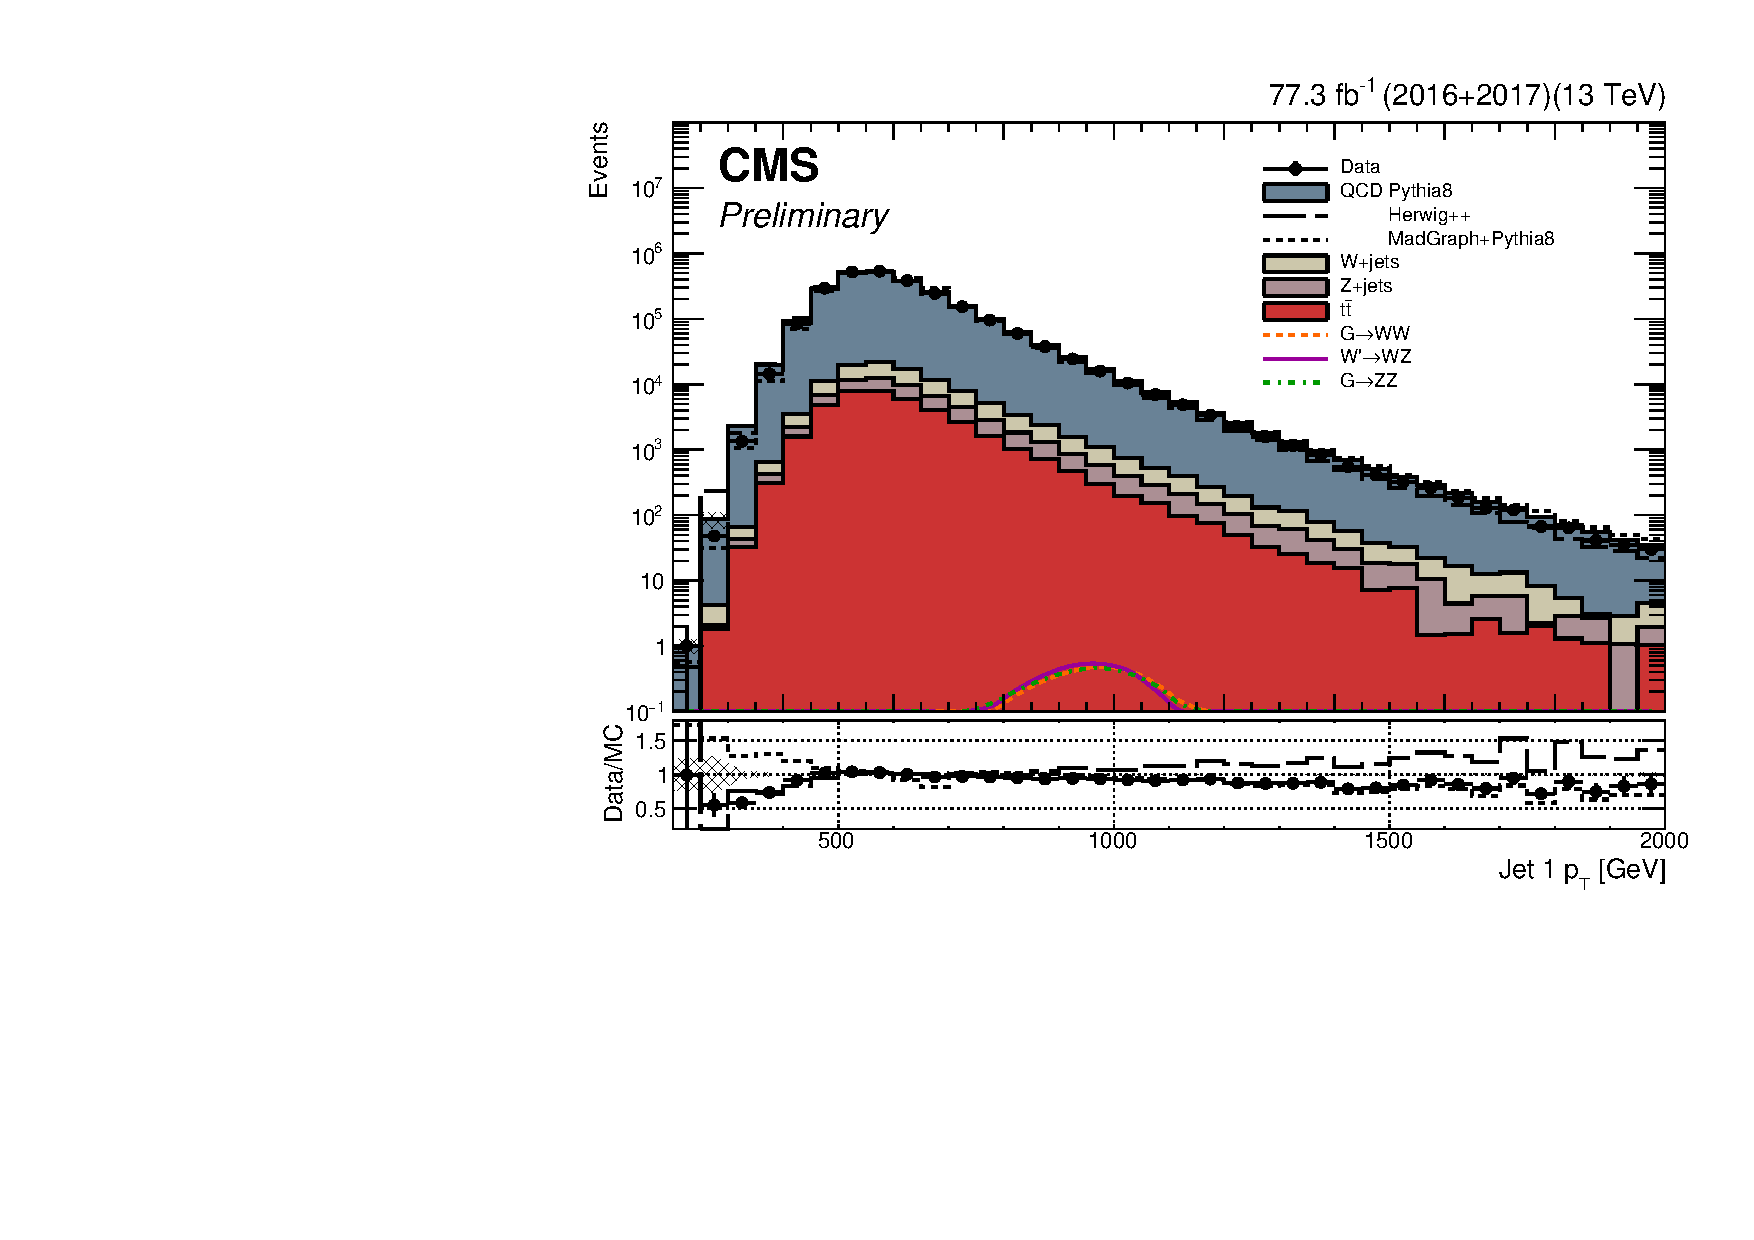
\includegraphics[width=0.450\textwidth]{figures/analysis/search3/AN-17-303/controlPlots/looseSel_Jet_1_p_T.pdf}
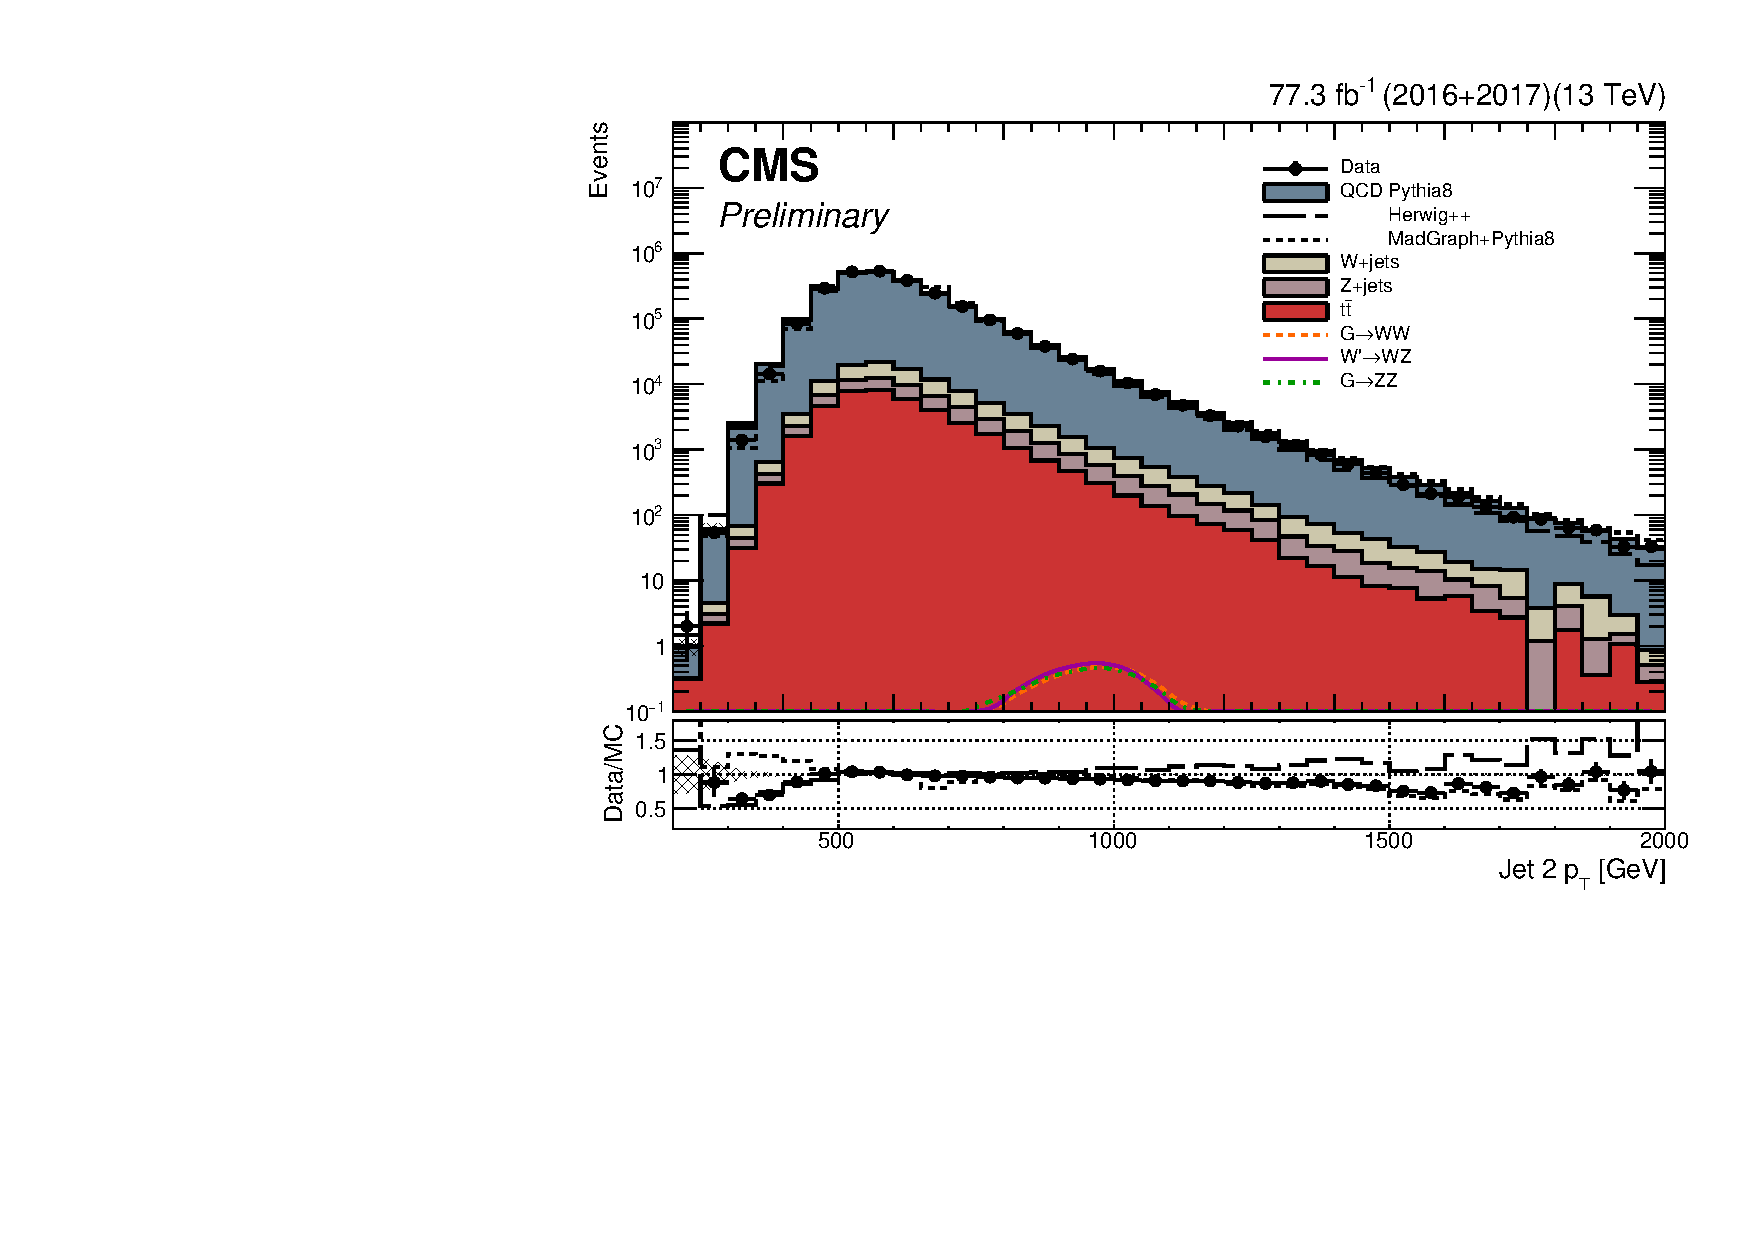
\includegraphics[width=0.450\textwidth]{figures/analysis/search3/AN-17-303/controlPlots/looseSel_Jet_2_p_T.pdf}\\
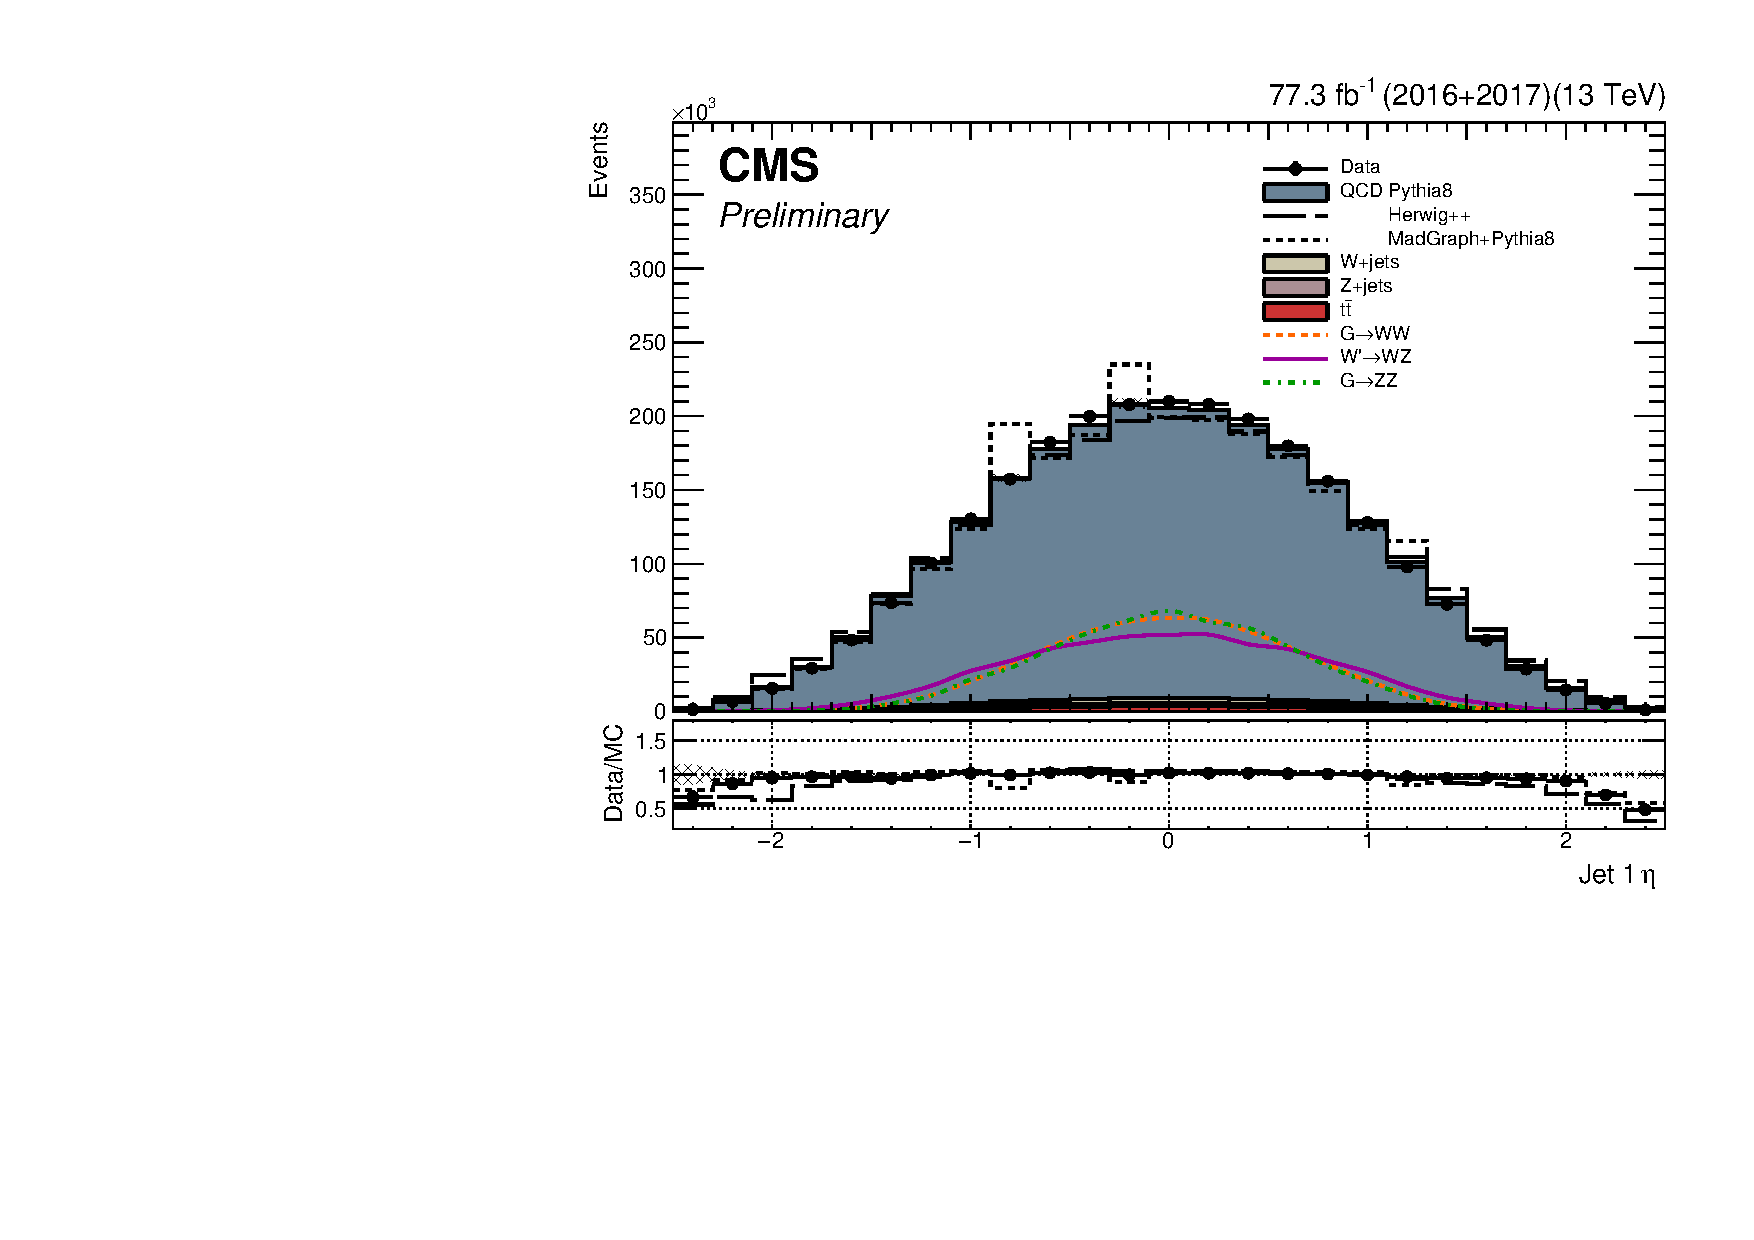
\includegraphics[width=0.450\textwidth]{figures/analysis/search3/AN-17-303/controlPlots/looseSel_Jet_1_eta.pdf}
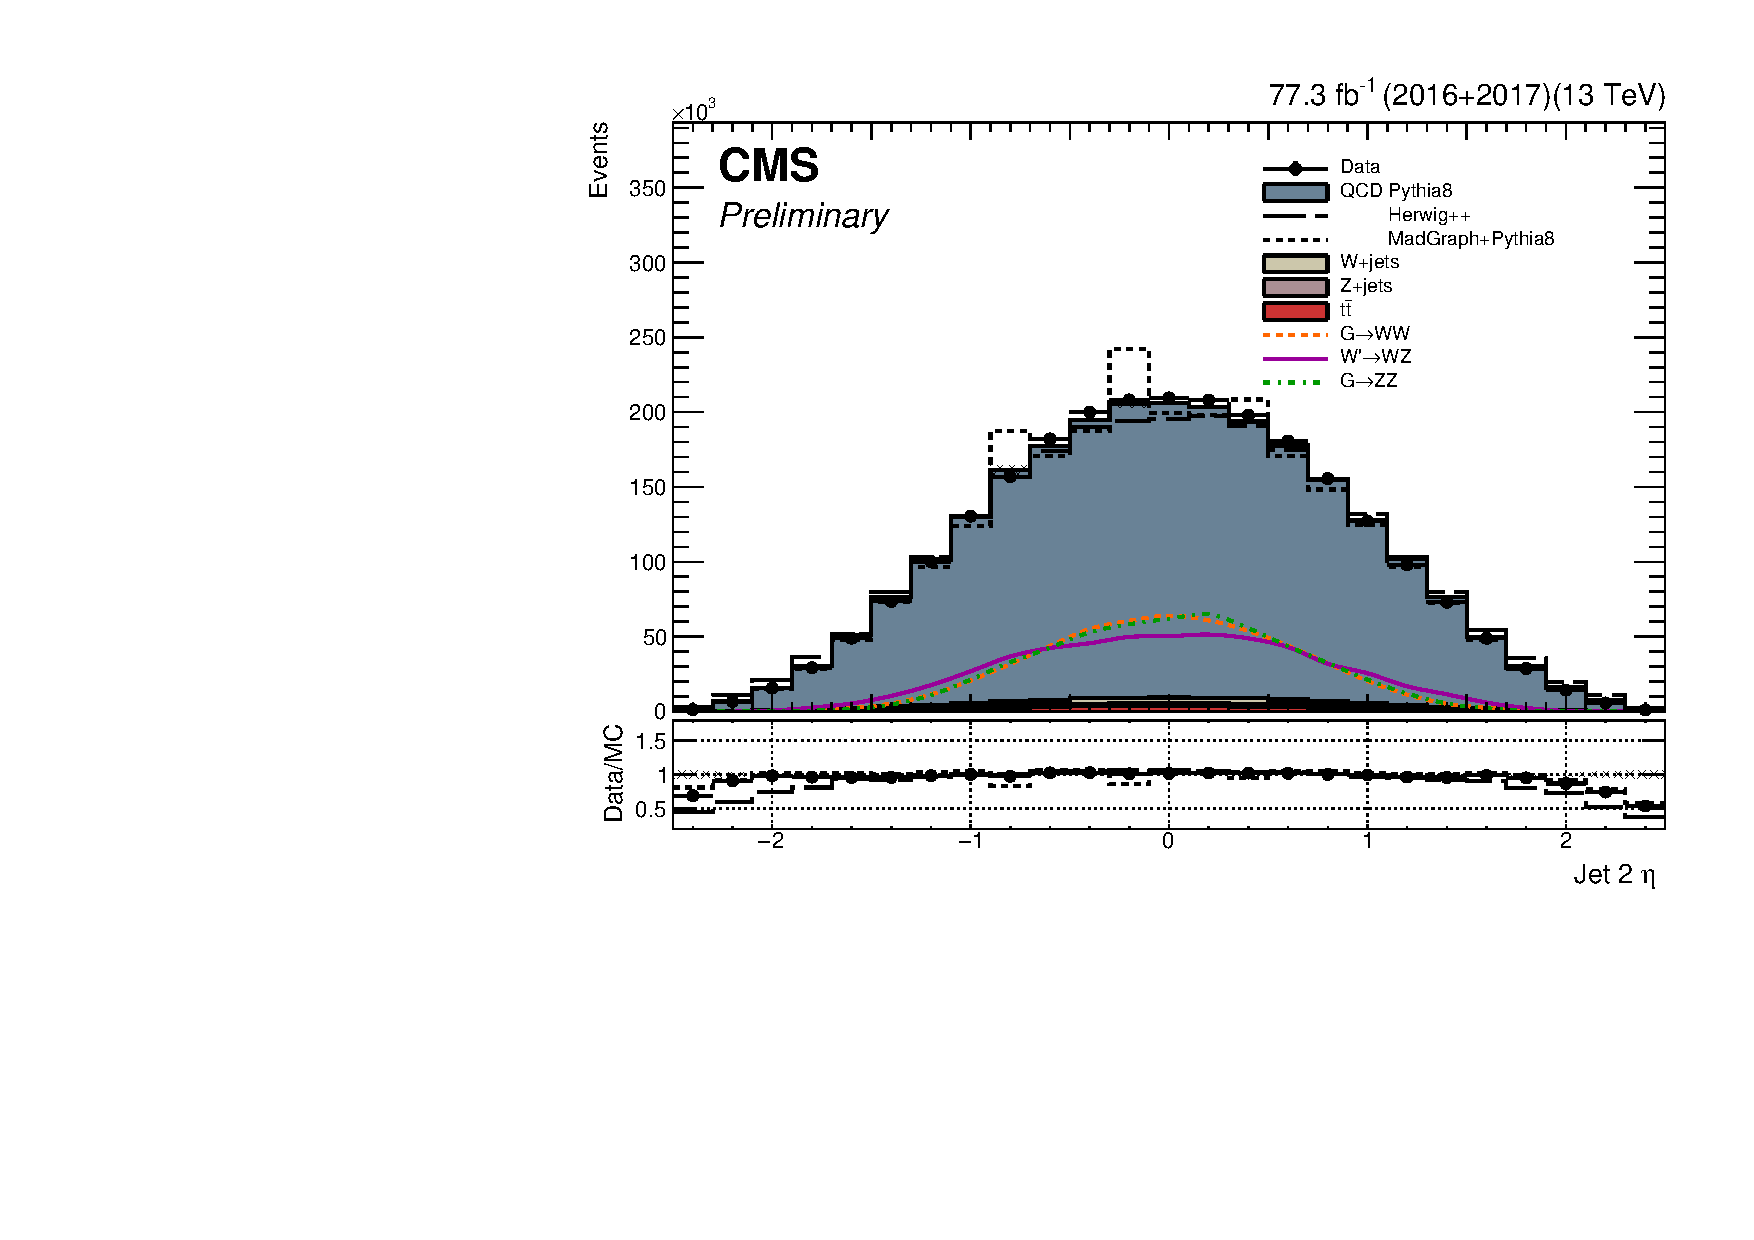
\includegraphics[width=0.450\textwidth]{figures/analysis/search3/AN-17-303/controlPlots/looseSel_Jet_2_eta.pdf}
\caption{Jet \PT{} (top) and $\eta$ (bottom) of the leading (left) and second leading (right) jet in the event. The signal is scaled by an arbitrary number.}
\label{fig:kinematics-all}
\end{figure}

\subsection{Triggering}
\label{sec:searchIII:trigger}
The triggers used for 2016 data are the same as in Section~\ref{sec:searchI:trigger}, while the thresholds in 2017 have increased in order to push the trigger rate to a level acceptable for the increased luminosity. The triggers used for 2017 data are
\begin{itemize}
\item \texttt{HLT\_PFHT1050}
\item \texttt{HLT\_AK8PFJet500}
\item \texttt{HLT\_AK8PFJet360/380/400/420\_TrimMass30}
\item \texttt{HLT\_AK8PFHT750/800/850/900\_TrimMass50}
\end{itemize}.
For the results presented here, the analysis threshold is set by the trigger turn-on point (where the combination of all triggers are $>99$ percent efficient). The trigger turn-on is evaluated in the Single Muon dataset, using the \texttt{HLT\_Mu50} and \texttt{HLT\_IsoMu27} triggers as reference triggers.  The trigger turn-on curves as a function of dijet invariant mass and jet soft drop mass are shown in Figure~\ref{fig:searchIII:trigturnon}.
The combination of all triggers are $>99\%$ efficient above a dijet invariant mass of 1126\GeV and this sets the analysis threshold. 
\begin{figure}[htb]
\centering 
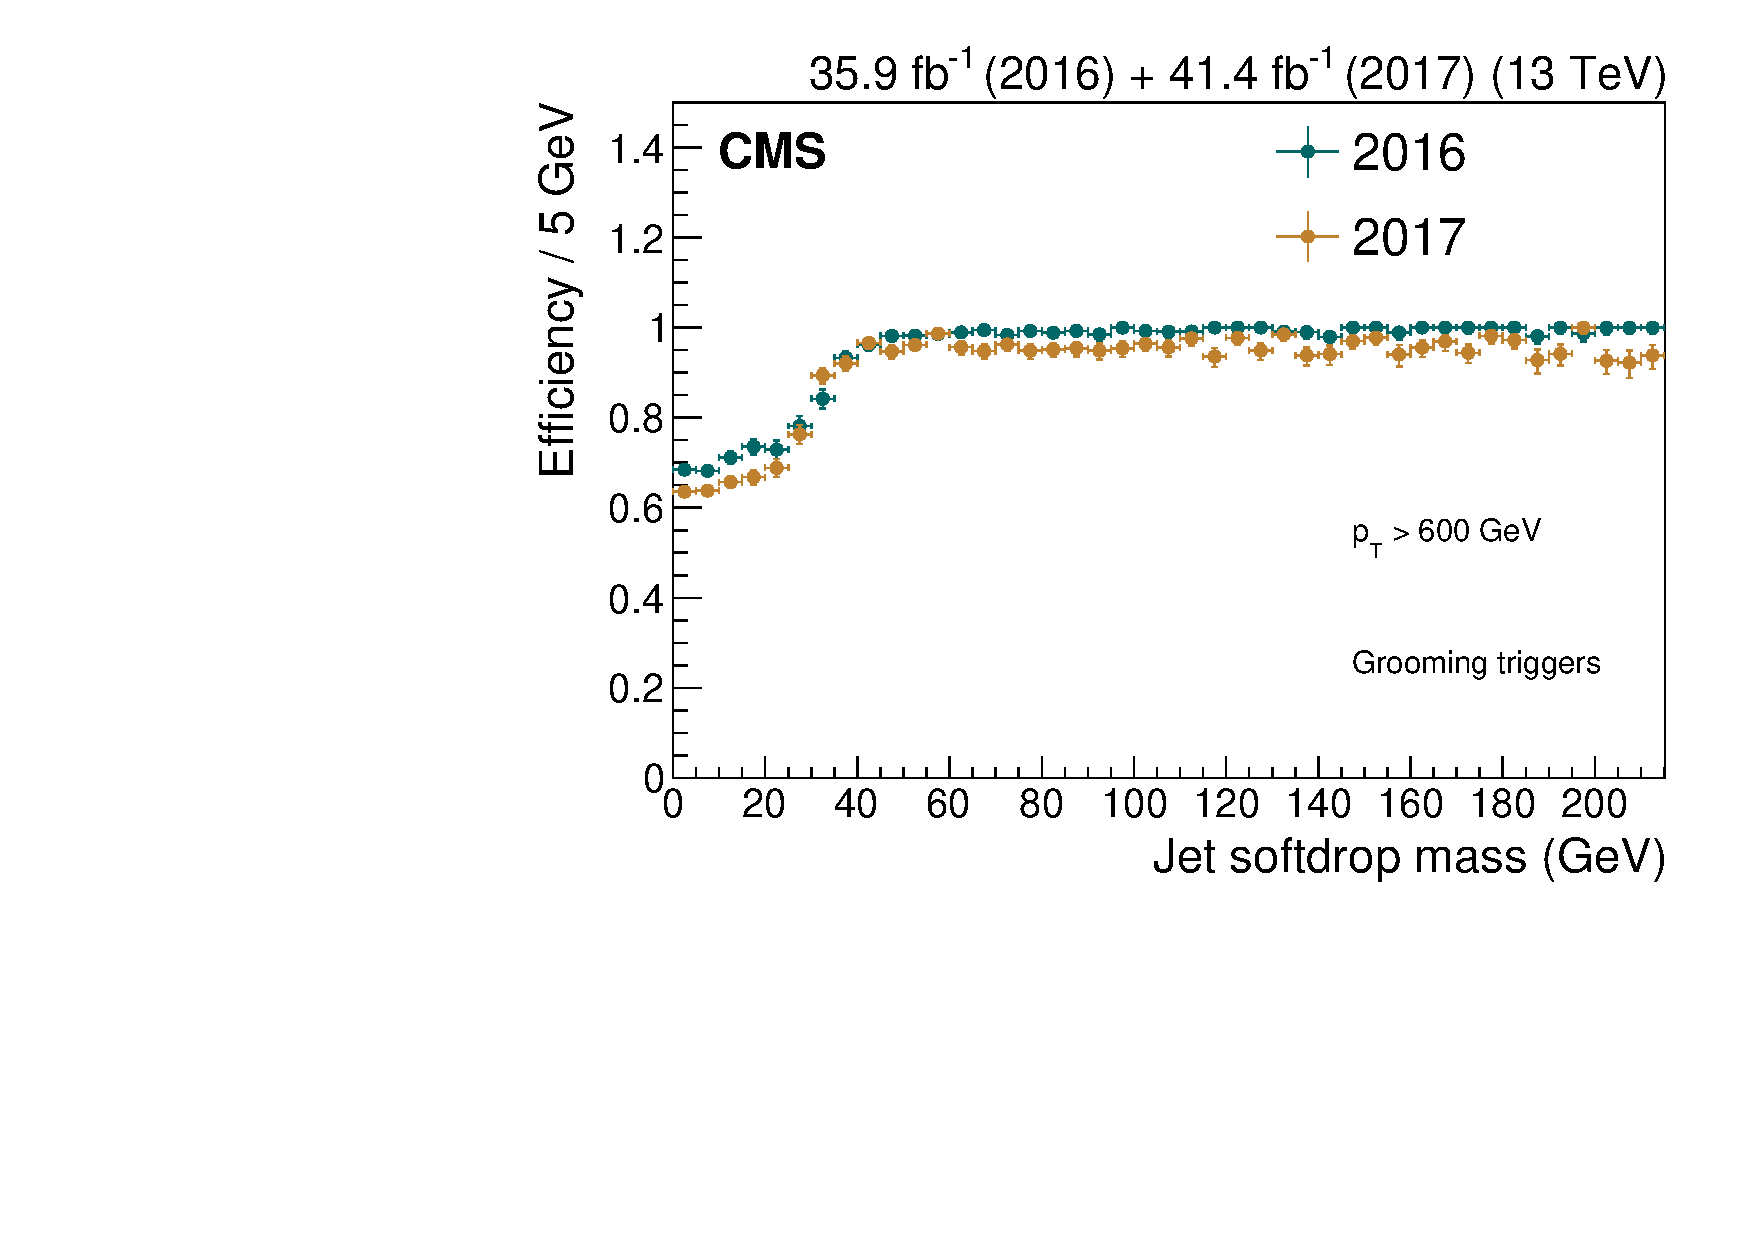
\includegraphics[width=0.45\textwidth]{figures/analysis/search3/B2G-18-002/Combined_mj1_16vs17.pdf}
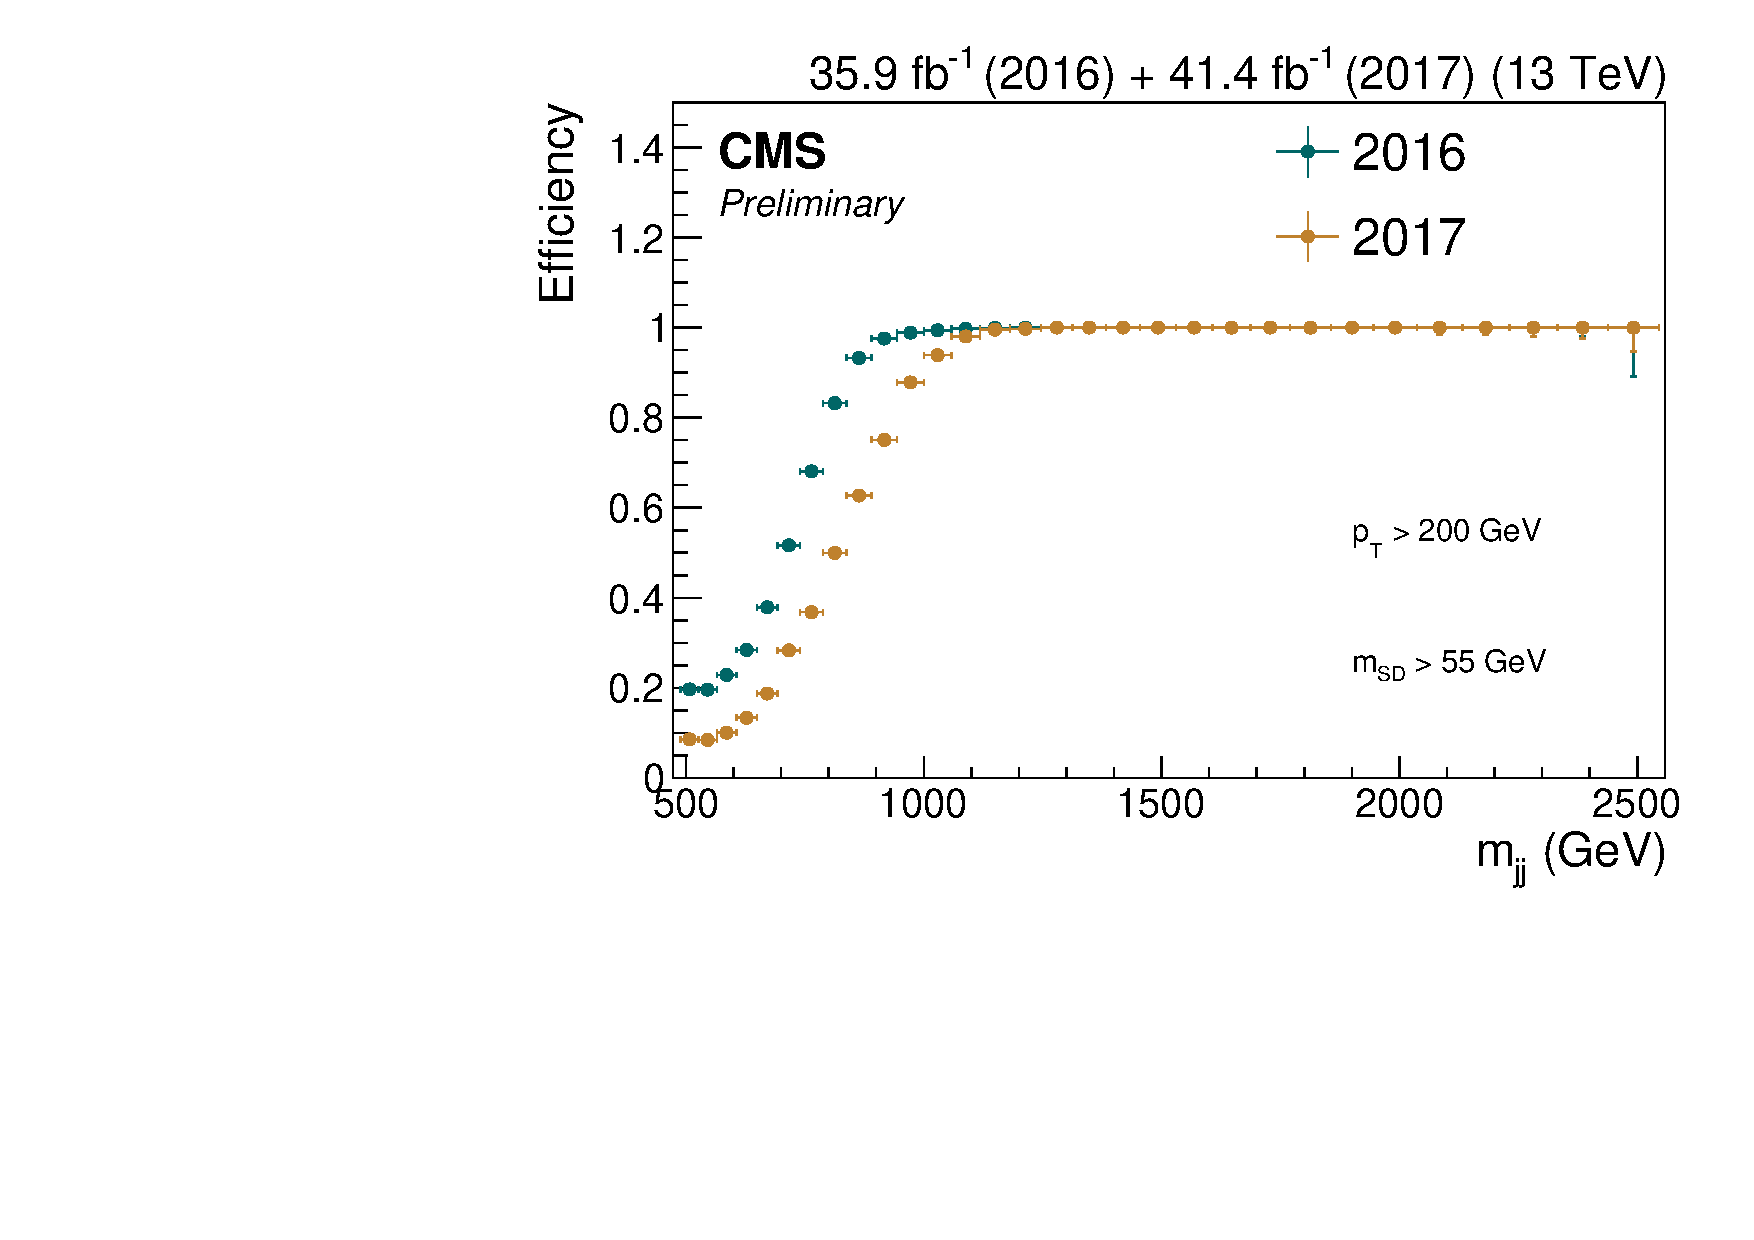
\includegraphics[width=0.45\textwidth]{figures/analysis/search3/B2G-18-002/Combined_mjj_16vs17.pdf}
\caption{Trigger turn-on curves in the 2016 and 2017 datasets for the \HT based (left) and groomed mass based (right) trigger paths.}
\label{fig:searchIII:trigturnon}
\end{figure}

\subsubsection{Trigger turn-on modeling}
\label{sec:searchIII:triggermodeling}
The analysis threshold for searches depending on the dijet fit is set by the trigger turn-on point as the analysis relies on a background fit of the dijet invariant mass spectrum with a smoothly falling function. As the background modeling for this analysis does not depend on a smoothly falling spectrum (as will be described in detail in Section~\ref{sec:searchIII:fit3d}), and in order to compensate for a loss in acceptance due to increased trigger thresholds, we attempted to model the trigger turn-on directly from data and apply a trigger weight in simulation.
To do so, we first study the one dimensional trigger turn-ons versus dijet invariant mass and softdrop jet mass to understand where in $\MVV$ and $\MJO$/$\MJT$ the triggers are fully efficient. We then derive a three dimensional histogram of the trigger efficiency versus dijet invariant mass ($\MVV$) and the jet groomed mass of jet 1 and jet 2 ($\MJO$ and $\MJT$), where each bin corresponds to the trigger efficiency for a given value of $\MVV$-$\MJO$-$\MJT$. The procedure is as follows: From the one dimensional histograms, the points of full efficiency versus $\MVV$, $\MJO$ and $\MJT$
are defined. For every bin above this threshold, the trigger efficiency is fixed to one (100 percent efficiency). For all bins below this trigger threshold, we fit slices of $\MVV$ with a sigmoid function, evaluate the trigger weights from this function, and set the bin content of
the three dimensional weight histogram accordingly. For every bin below this point, the trigger weight is extracted by fitting slices of $\MVV$ in each bin of $\MJO/\MJT$.
As the trigger efficiency falls below 50 percent around a dijet invariant mass of 800 GeV (Figure~\ref{fig:searchIII:trigturnon}), searching for resonances with masses below this point is non-feasible. In addition, the full signal shape needs to be contained within the dijet invariant mass spectrum, excluding resonance masses of 0.8 and 0.9 TeV. The lowest mass point signal sample to set limits on for this analysis is therefore at 1 TeV and the analysis threshold is fixed at $\MVV = $900 GeV in order to fully contain the signal shape.
Starting from $\MVV=893$ GeV (dijet bin closest to 900 GeV) and $\MJO/\MJT=40$ GeV, a coarsely binned three-dimensional histogram (10 GeV $\MJO/\MJT$ binning and "dijet" binning in $\MVV$) is filled with the fraction of events that pass one of the signal triggers,
\begin{equation*}
w^{Bin}_{ijk}= \frac{\textrm{ PASS}\big(m_{jj}^i-m_{j1}^j-m_{j2}^k\big) }{\textrm{ ALL}\big(m_{jj}^i-m_{j1}^j-m_{j2}^k\big)}.
\end{equation*}
The resulting coarse histogram is then expanded in $\MVV$ to 10 GeV dijet invariant mass bins, interpolating between the points using sigmoid fit for each $\MJO-\MJT$ bin (the fine binning in dijet invariant mass is sufficient enough to yield a smooth reweighted distribution so no expansion is done in $\MJO/\MJT$).
% This three-dimensional coarse weight histogram is illustrated in Figure~\ref{fig:3Dtrigger}.
% \begin{figure}[htb]
% \centering
% 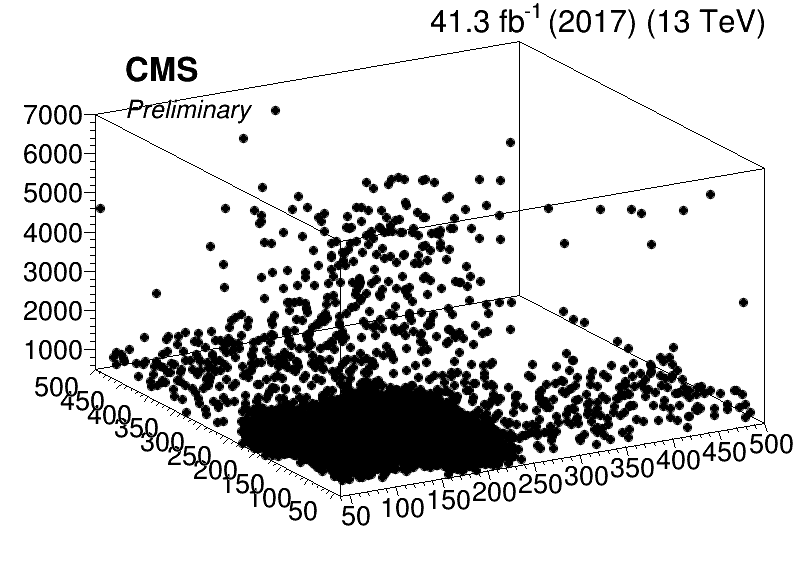
\includegraphics[width=0.45\textwidth]{figures/analysis/search3/AN-17-303/trigger/3D_interpolate.png}
% \caption{Trigger efficiency (coarse) in the three-dimensional $\MVV$-$\MJO$-$\MJT$ plane. }
% \label{fig:3Dtrigger}
% \end{figure}
From this histogram, each slice in $\MVV$ is fitted with a sigmoid function,
\begin{equation*}
s(x)=\frac{1}{1+e^{-p_1(x-p_2)}}
\end{equation*}
the trigger weight of each bin $\MVV$-$\MJO$-$\MJT$ is extracted from the fit and set accordingly.
% An example of two such fits and their corresponding trigger weight in projections of $\MVV$ is shown in Figure~\ref{fig:triggerWeights}.
% \begin{figure}[htb]
% \centering
% 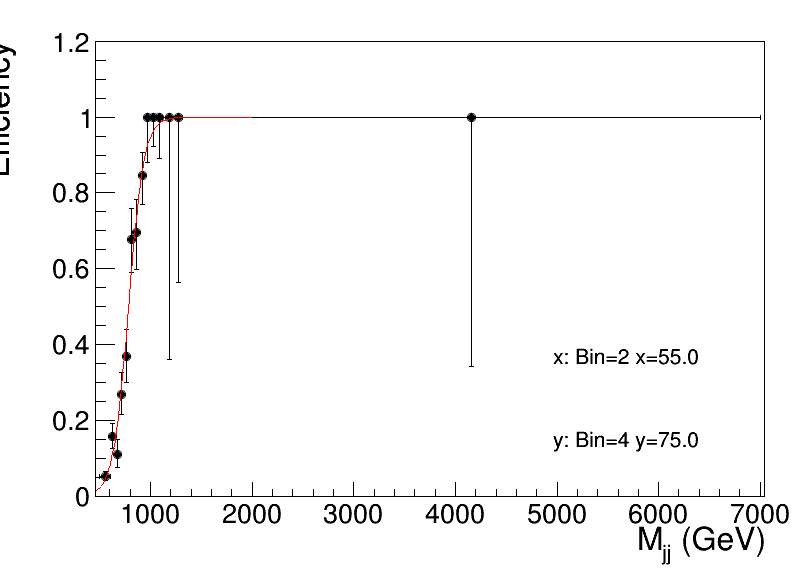
\includegraphics[height=3cm]{figures/analysis/search3/AN-17-303/trigger/x2_y4_fitstatus0.png}
% 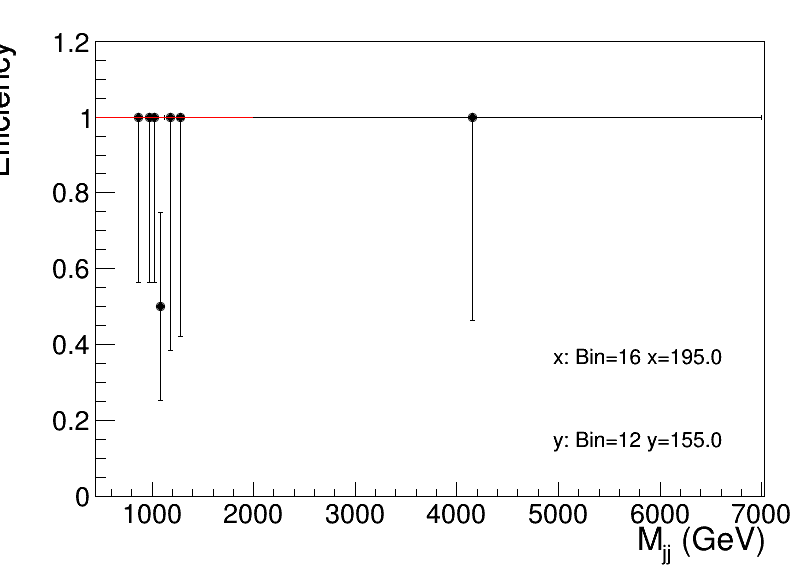
\includegraphics[height=3cm]{figures/analysis/search3/AN-17-303/trigger/x16_y12_fitstatus0.png}\\
% 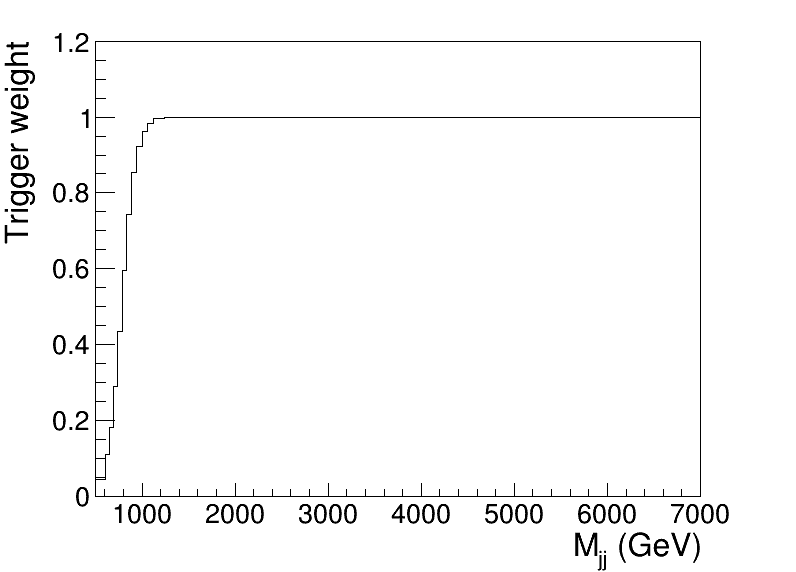
\includegraphics[height=3cm]{figures/analysis/search3/AN-17-303/trigger/x2_y4_weight.png}
% 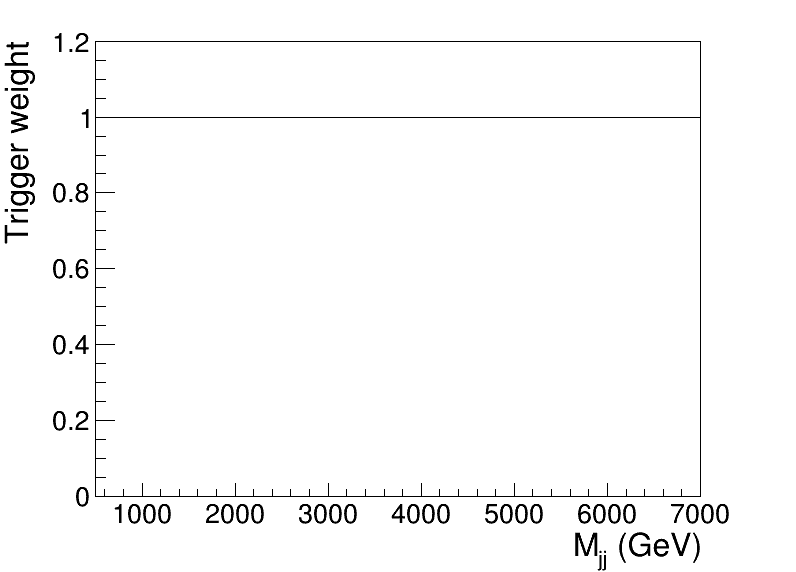
\includegraphics[height=3cm]{figures/analysis/search3/AN-17-303/trigger/x16_y12_weight.png}
% \caption{Fits to the trigger efficiency in slices of $\MVV$ for (top left) a central ($\MJO=55 \GeV$, $\MJT=75 \GeV$) and (top right) an extreme ($\MJO=195 \GeV$, $\MJT=155 \GeV$) bin (top)
% and the corresponding trigger weights derived from the fit (bottom).}
% \label{fig:triggerWeights}
% \end{figure}
Figure~\ref{fig:triggerProj} shows the total projections on each axis for the full trigger weight histogram.
\begin{figure}[htb]
\centering
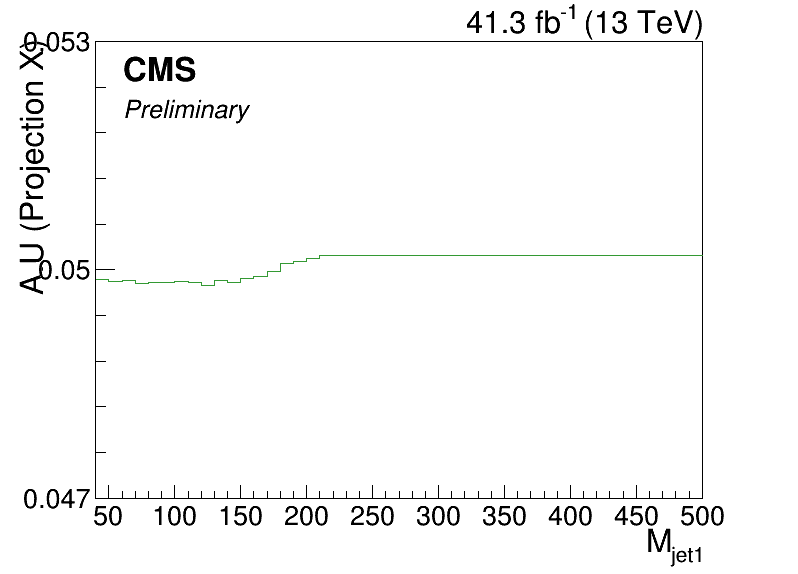
\includegraphics[width=0.3\textwidth]{figures/analysis/search3/AN-17-303/trigger/3D_x.png}
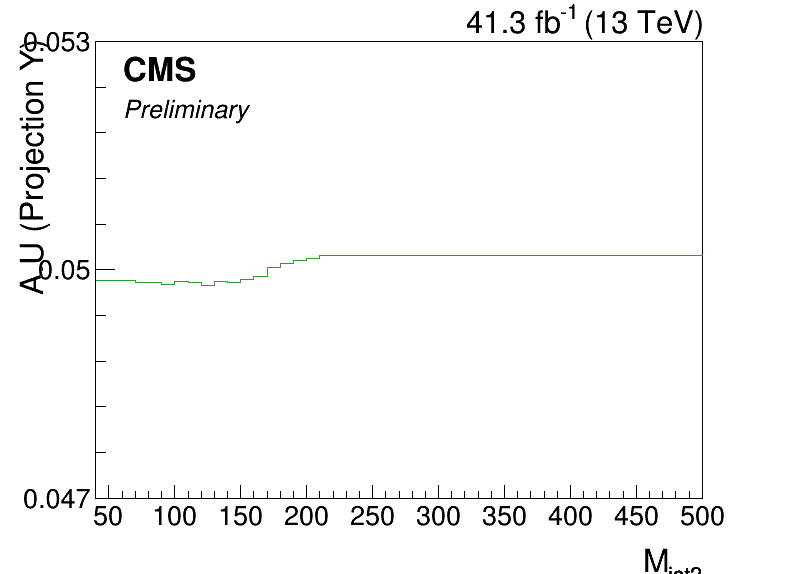
\includegraphics[width=0.3\textwidth]{figures/analysis/search3/AN-17-303/trigger/3D_y.png}
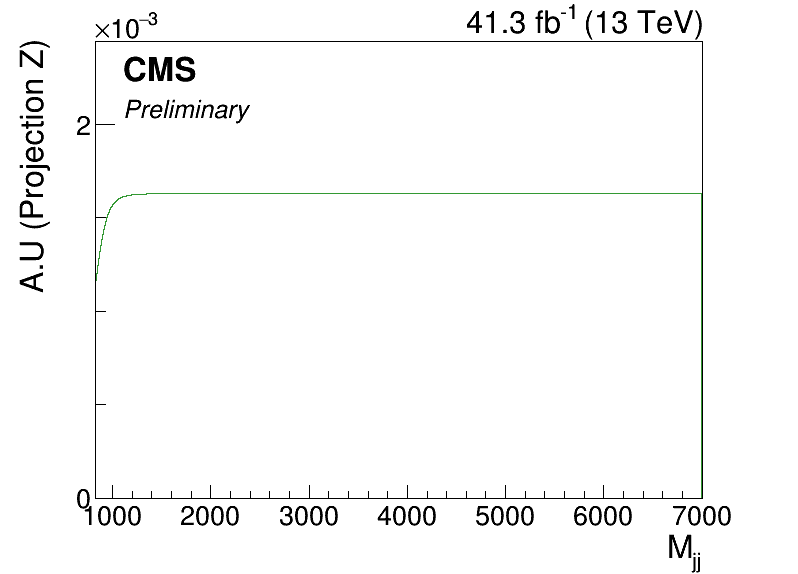
\includegraphics[width=0.3\textwidth]{figures/analysis/search3/AN-17-303/trigger/3D_z.png}
% 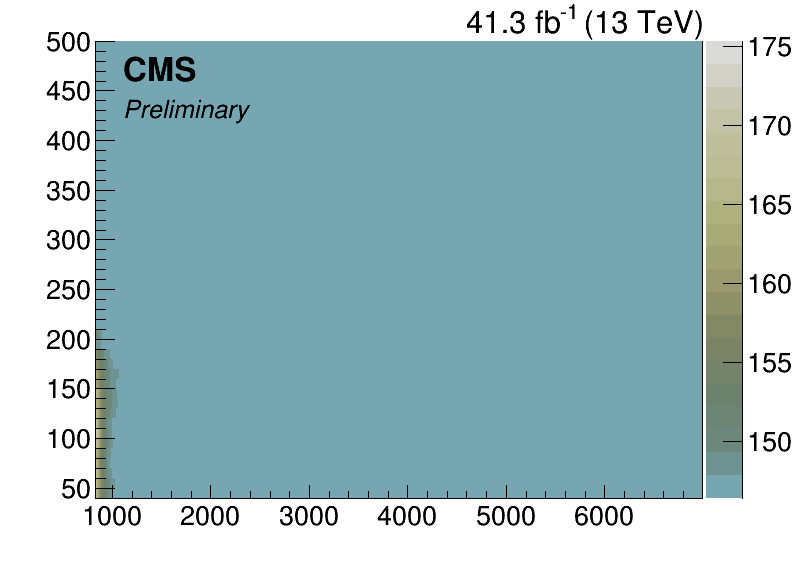
\includegraphics[width=0.3\textwidth]{figures/analysis/search3/AN-17-303/trigger/3D_yz.png}
% 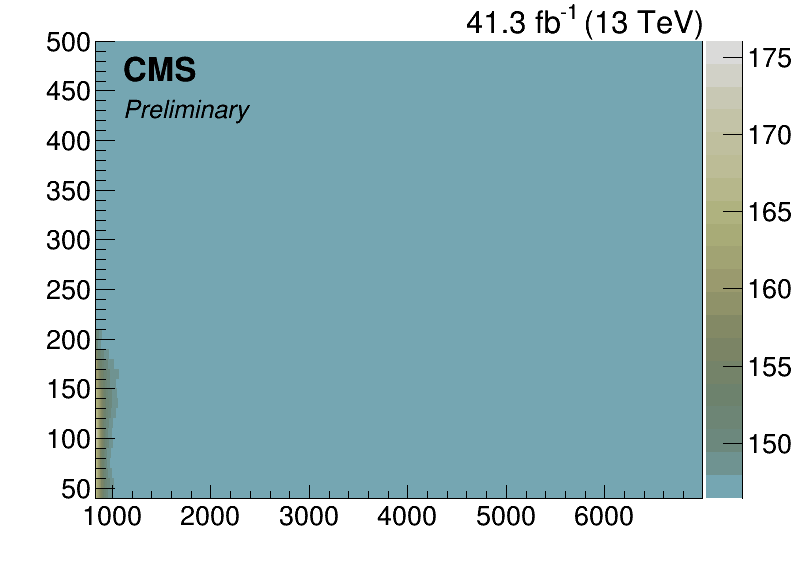
\includegraphics[width=0.3\textwidth]{figures/analysis/search3/AN-17-303/trigger/3D_xz.png}
% 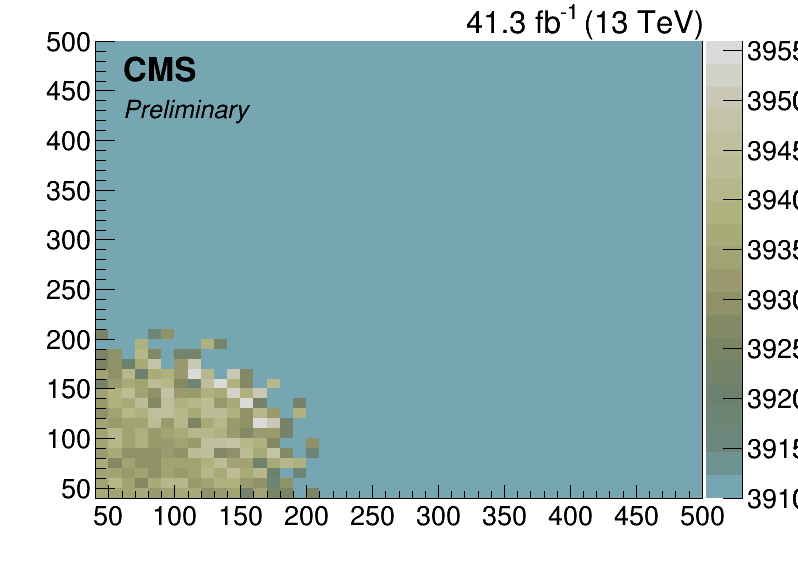
\includegraphics[width=0.3\textwidth]{figures/analysis/search3/AN-17-303/trigger/3D_yx.png}
\caption{One-dimensional projections of the trigger weight histogram for $\MJO$, $\MJT$ and $\MVV$ respectively.}
\label{fig:triggerProj}
\end{figure}
The $\MJ$ and $\MVV$ spectra for the lowest mass-point signal sample and for the QCD background before and after trigger weights are applied,
are shown in Figure~\ref{fig:triggerMCspectra} and are compared to data. $>95\%$ of the signal efficiency is retained, and reweighted QCD simulation agrees well with data.
\begin{figure}[h!]
\centering
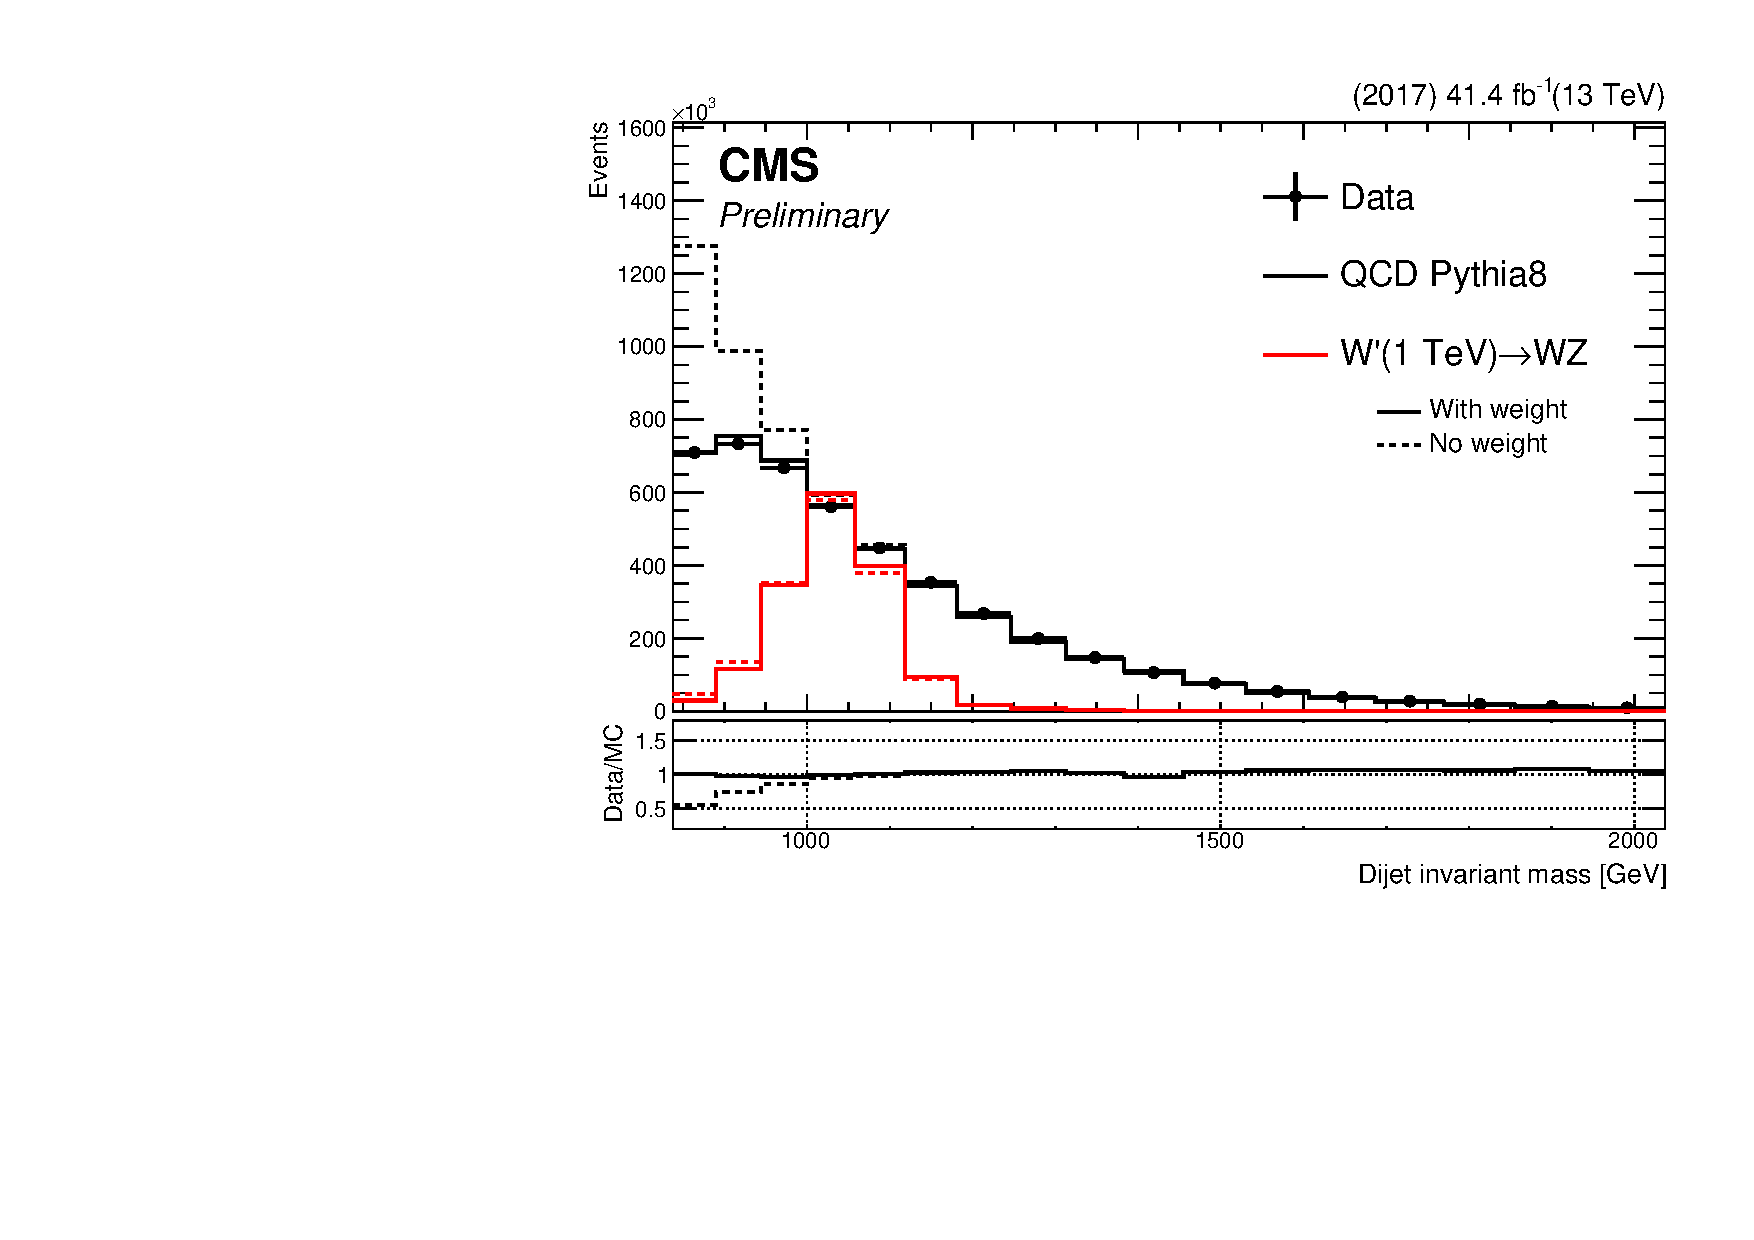
\includegraphics[width=0.49\textwidth]{figures/analysis/search3/B2G-18-002/trigWeightCompare_looseSel_Dijet_invariant_mass.pdf}
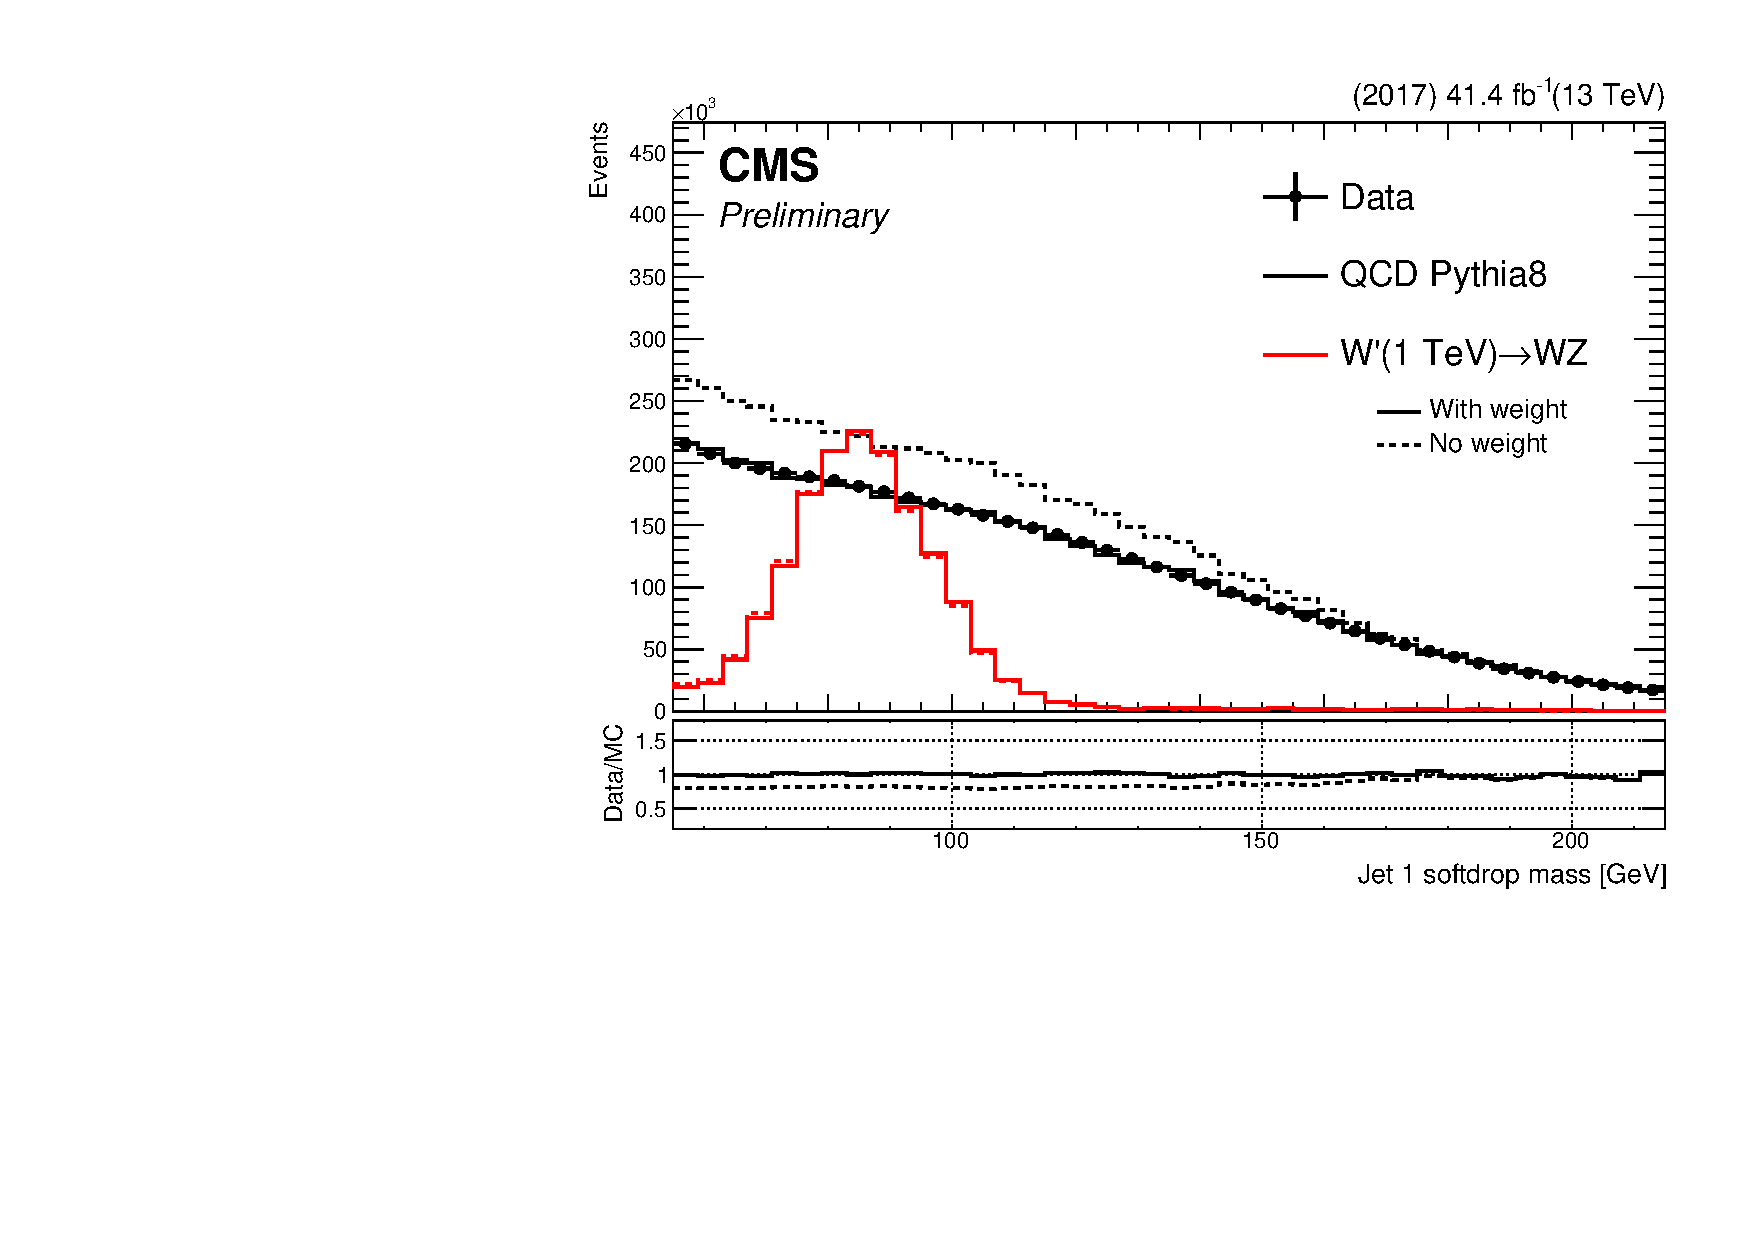
\includegraphics[width=0.49\textwidth]{figures/analysis/search3/B2G-18-002/trigWeightCompare_looseSel_Jet_1_softdrop_mass.pdf}
\caption{The $\MVV$ (left) and $\MJ$ (right) spectra for signal and background before and after trigger weights are applied.}
\label{fig:triggerMCspectra}
\end{figure}
The modeling of the trigger turn-on was successful and implemented in the background fit method in the 3D analysis. We found that the method could model the turn-on well. However, when studying the bias on the extracted signal rate for a possible signal in this turn-on region, we found that this was large due to us attempting to fit a peak on top of a peaky background. As we wanted this analysis describing the 3D fit method to become available as soon as possible, we therefore abandoned modeling of the trigger turn-on for this paper. However, we still wish to pursue this strategy in the future.
\clearpage

\subsection{A mass and \PT decorrelated tagger}
\label{sec:searchIII:ddt}
In order to identify W and Z jet candidates, two algorithms are run on the AK8 PUPPI jet: softdrop~\cite{softdrop} and the N-subjettiness ratio $\tau_{21}$~\cite{nsubjettiness}.
The softdropped jet mass is used to improve the mass resolution of the jet, while N-subjettiness serves as a discriminant by yielding a probability of how compatible the jet is with having N axes. For this search, we require the softdrop-jet mass to be in a window around the W/Z/H/top mass, between 55 and 215 GeV, something which we plan to extend in the future. In order to improve the statistical power of the jet substructure variable $\tau_{21}$ and ensure a minimal sculpting of the jet mass as a function of jet $p_T$,
we decorrelate the variable from the jet softdrop mass and the jet $p_T$-scale dependence following what was done in Ref.~\cite{ddt}.
This decorrelation is performed by flattening the $\tau_{21}$ profile dependence on $\rho' = log(m^2/p_T/\mu)$, where $\mu$ = 1 GeV.
Figure~\ref{fig:rho} shows the profile distribution of $\tau_{21}$ as a function of $\rho' = log(m^2/p_T/\mu)$, applying the preselections as listed above together with a softdrop mass cut of $\unit{55}{\GeV} < M_{jet} < \unit{215}{\GeV}$ (right).
% $\rho = log(m^2/p_T^2)$ (top) and as a function of $\rho' = log(m^2/p_T/\mu)$ (bottom), applying the preselections as listed in~\ref{sec:presel} (left) and after applying a softdrop mass cut of $\unit{55}{\GeV} < M_{jet} < \unit{215}{\GeV}$ (right).
\begin{figure}[htbp]
\centering
\begin{tabular}{cc}
% 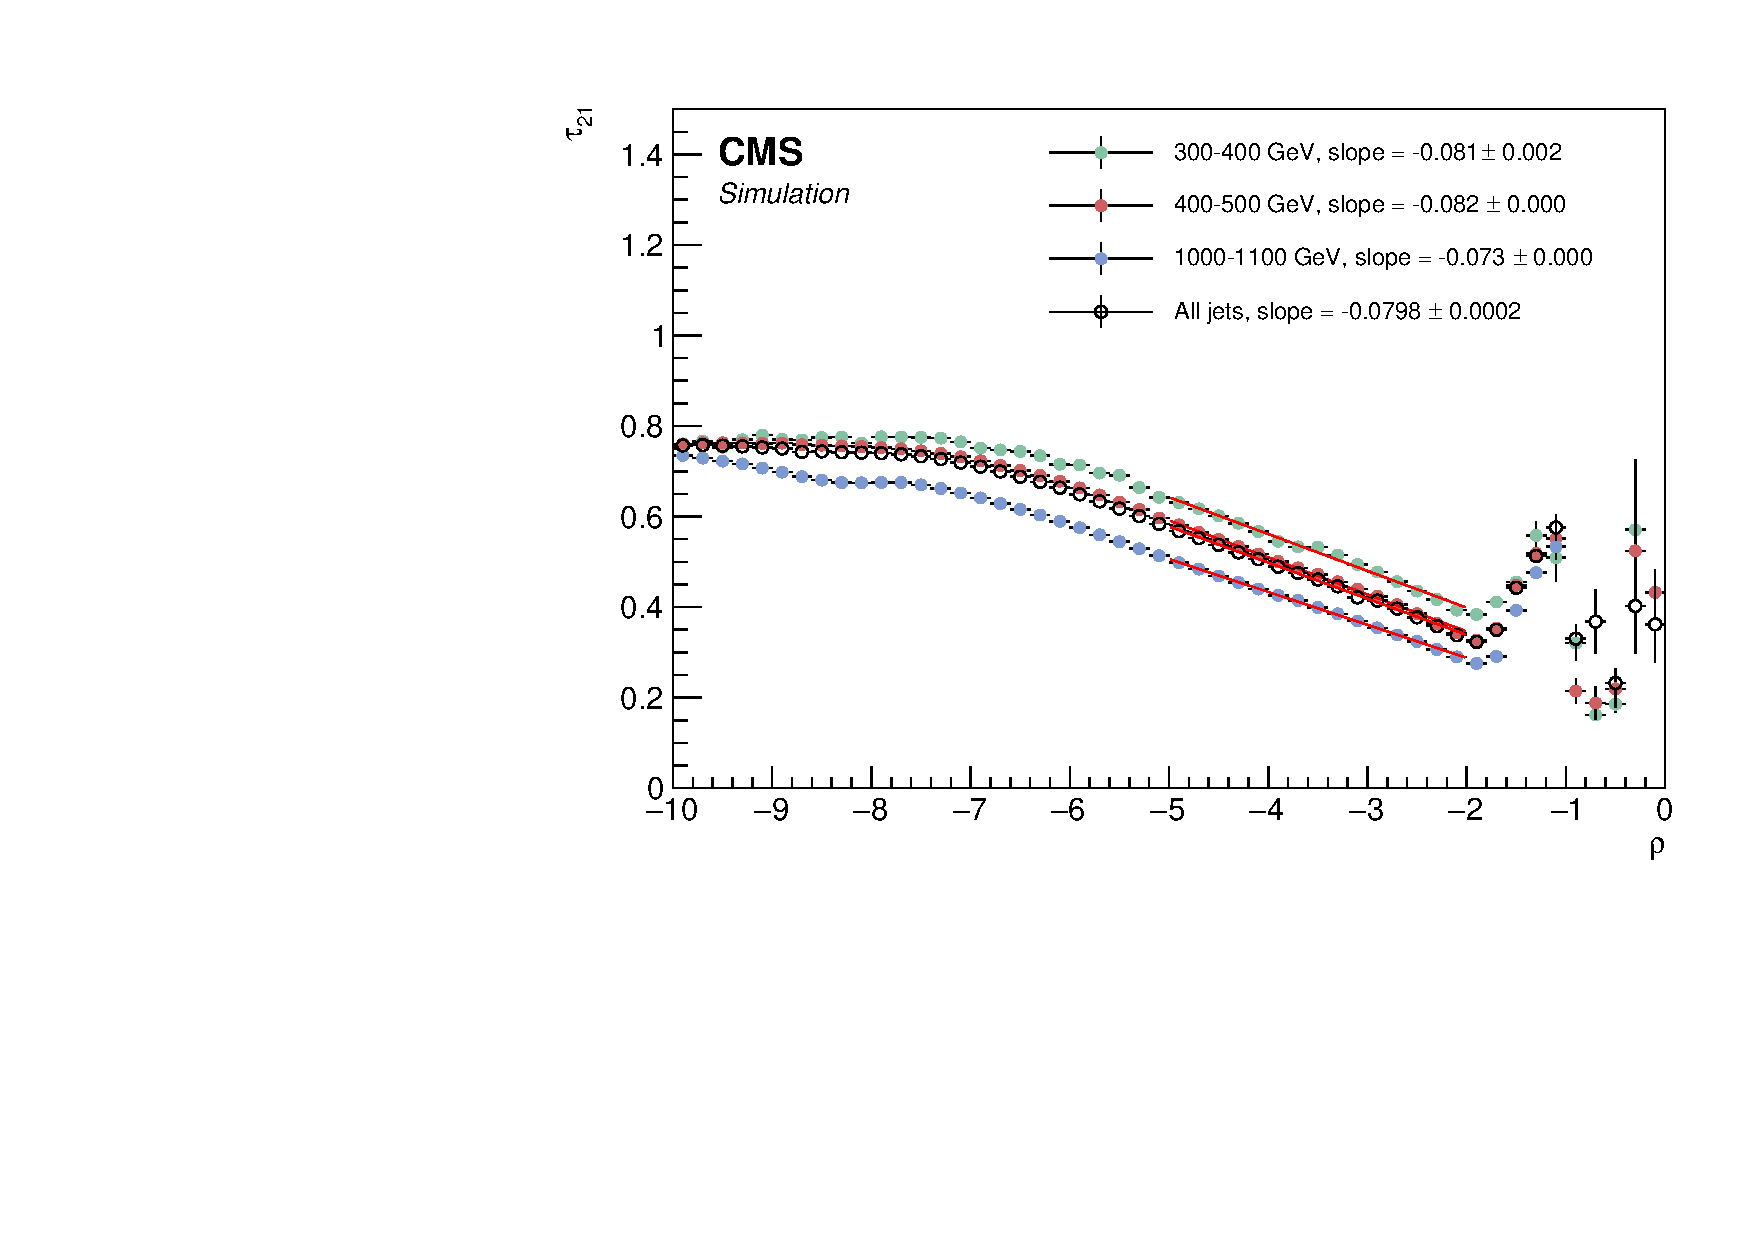
\includegraphics[width=0.45\textwidth]{figures/analysis/search3/AN-17-303/vtag/rho_pythia.pdf}
% 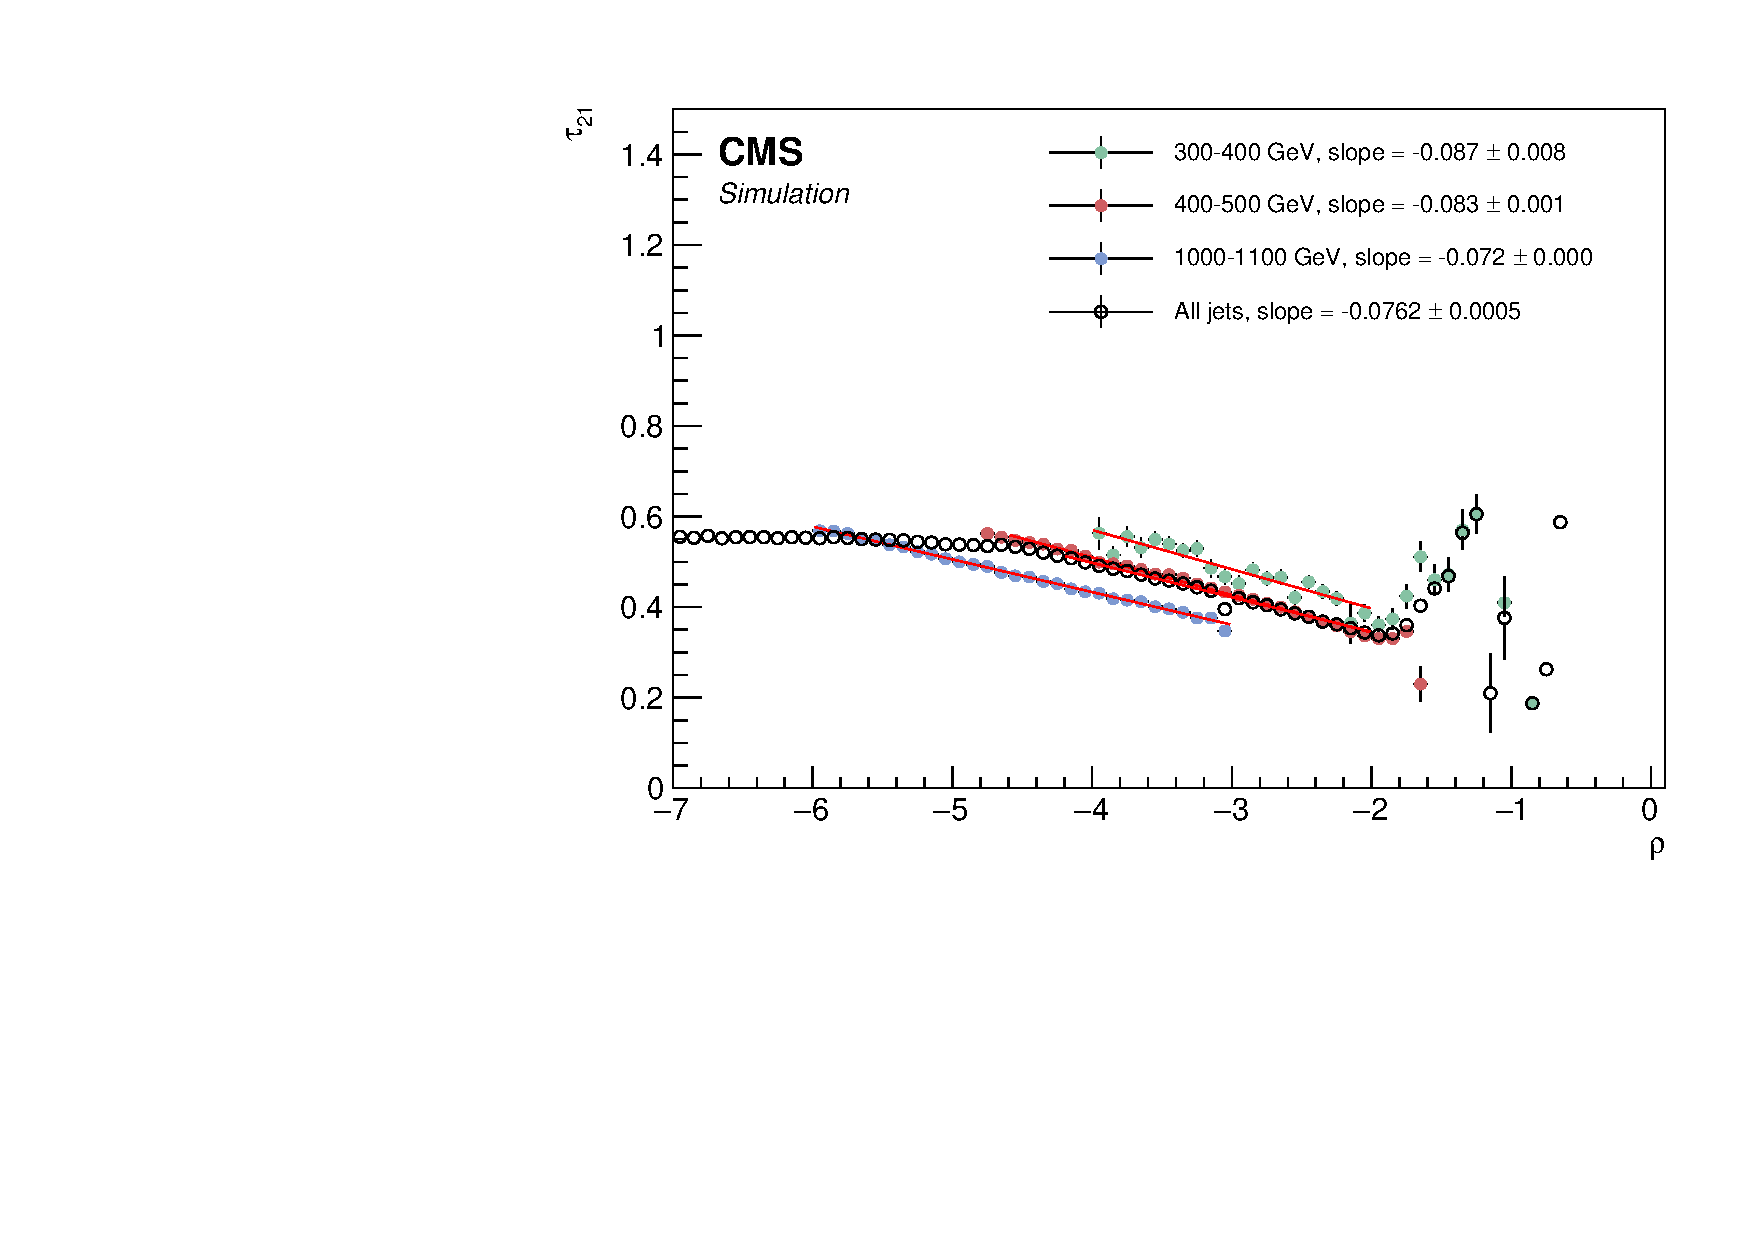
\includegraphics[width=0.45\textwidth]{figures/analysis/search3/AN-17-303/vtag/rho_pythia_FullSel.pdf}\\
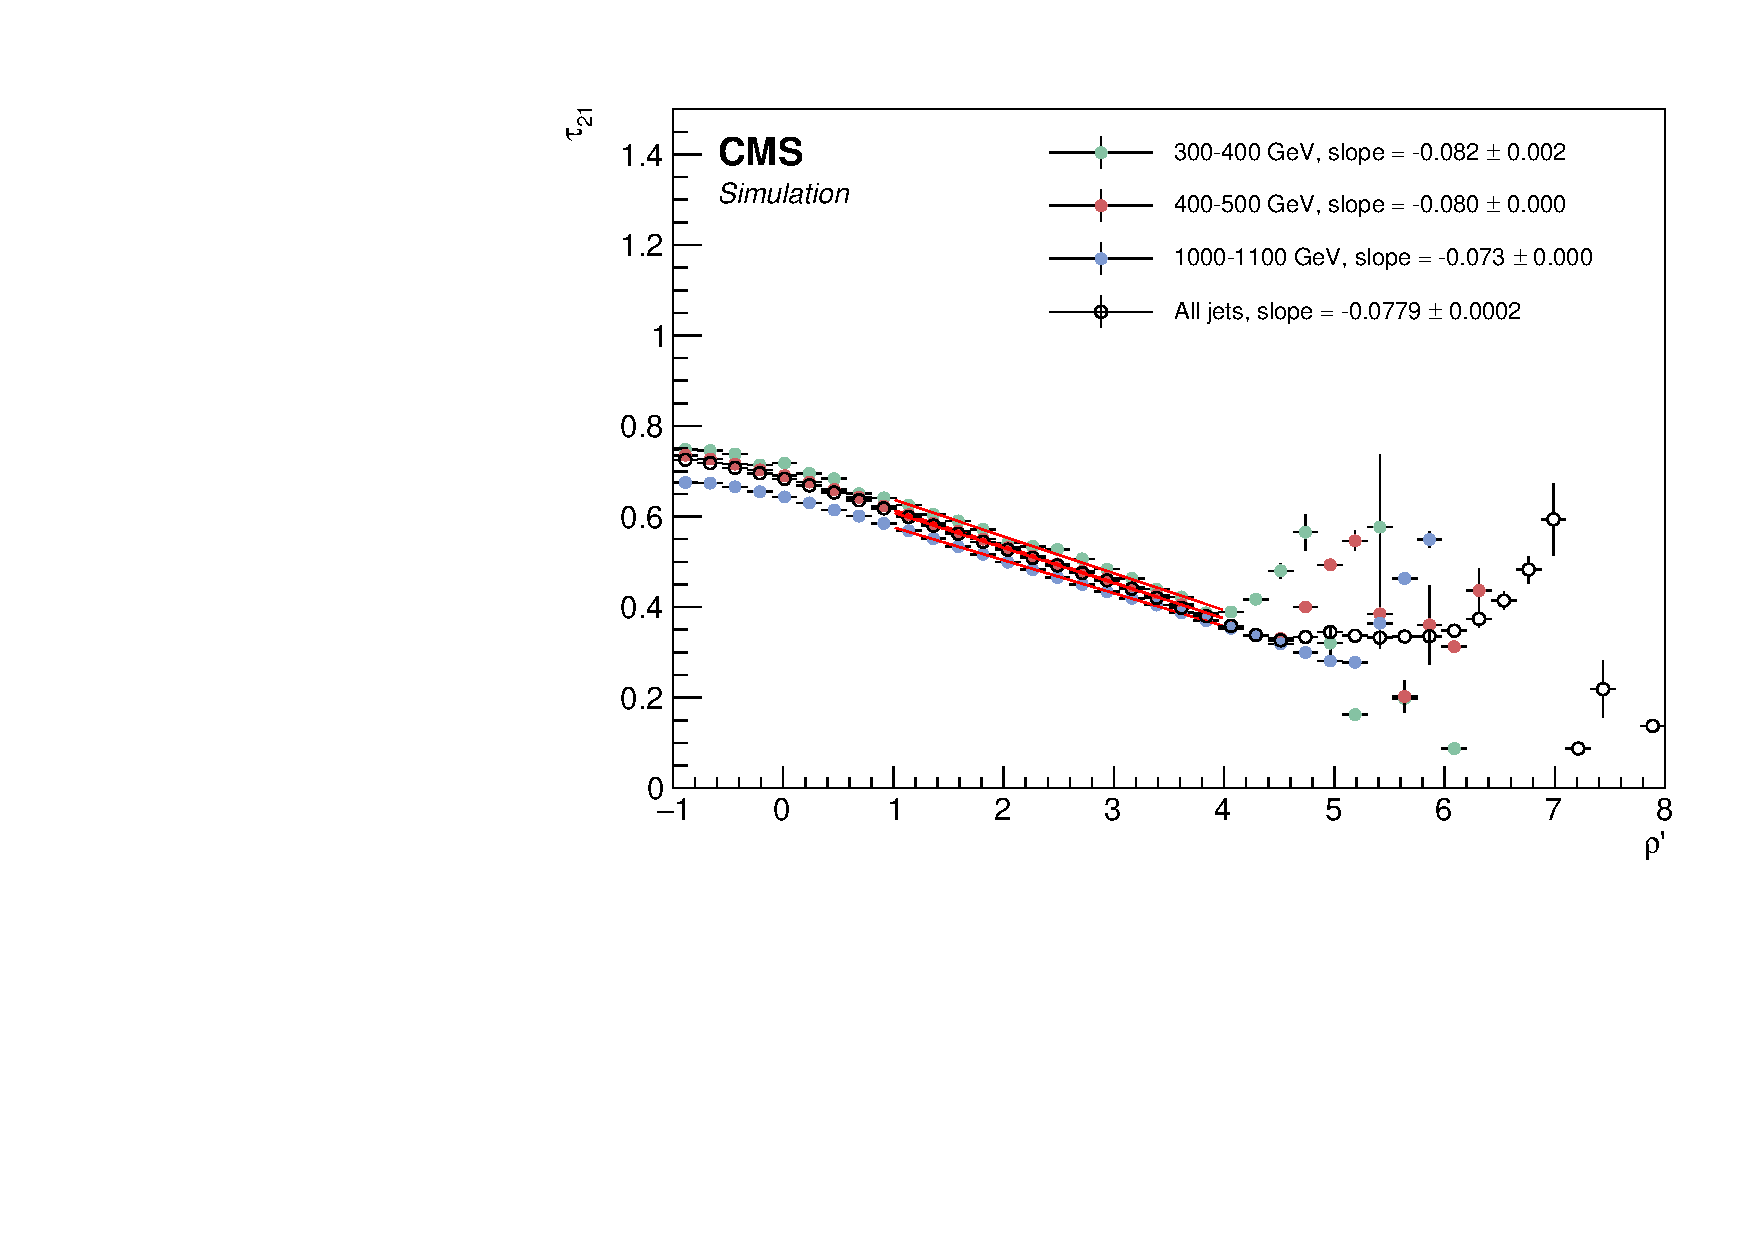
\includegraphics[width=0.45\textwidth]{figures/analysis/search3/AN-17-303/vtag/rho_pythia_rhoPrime.pdf}
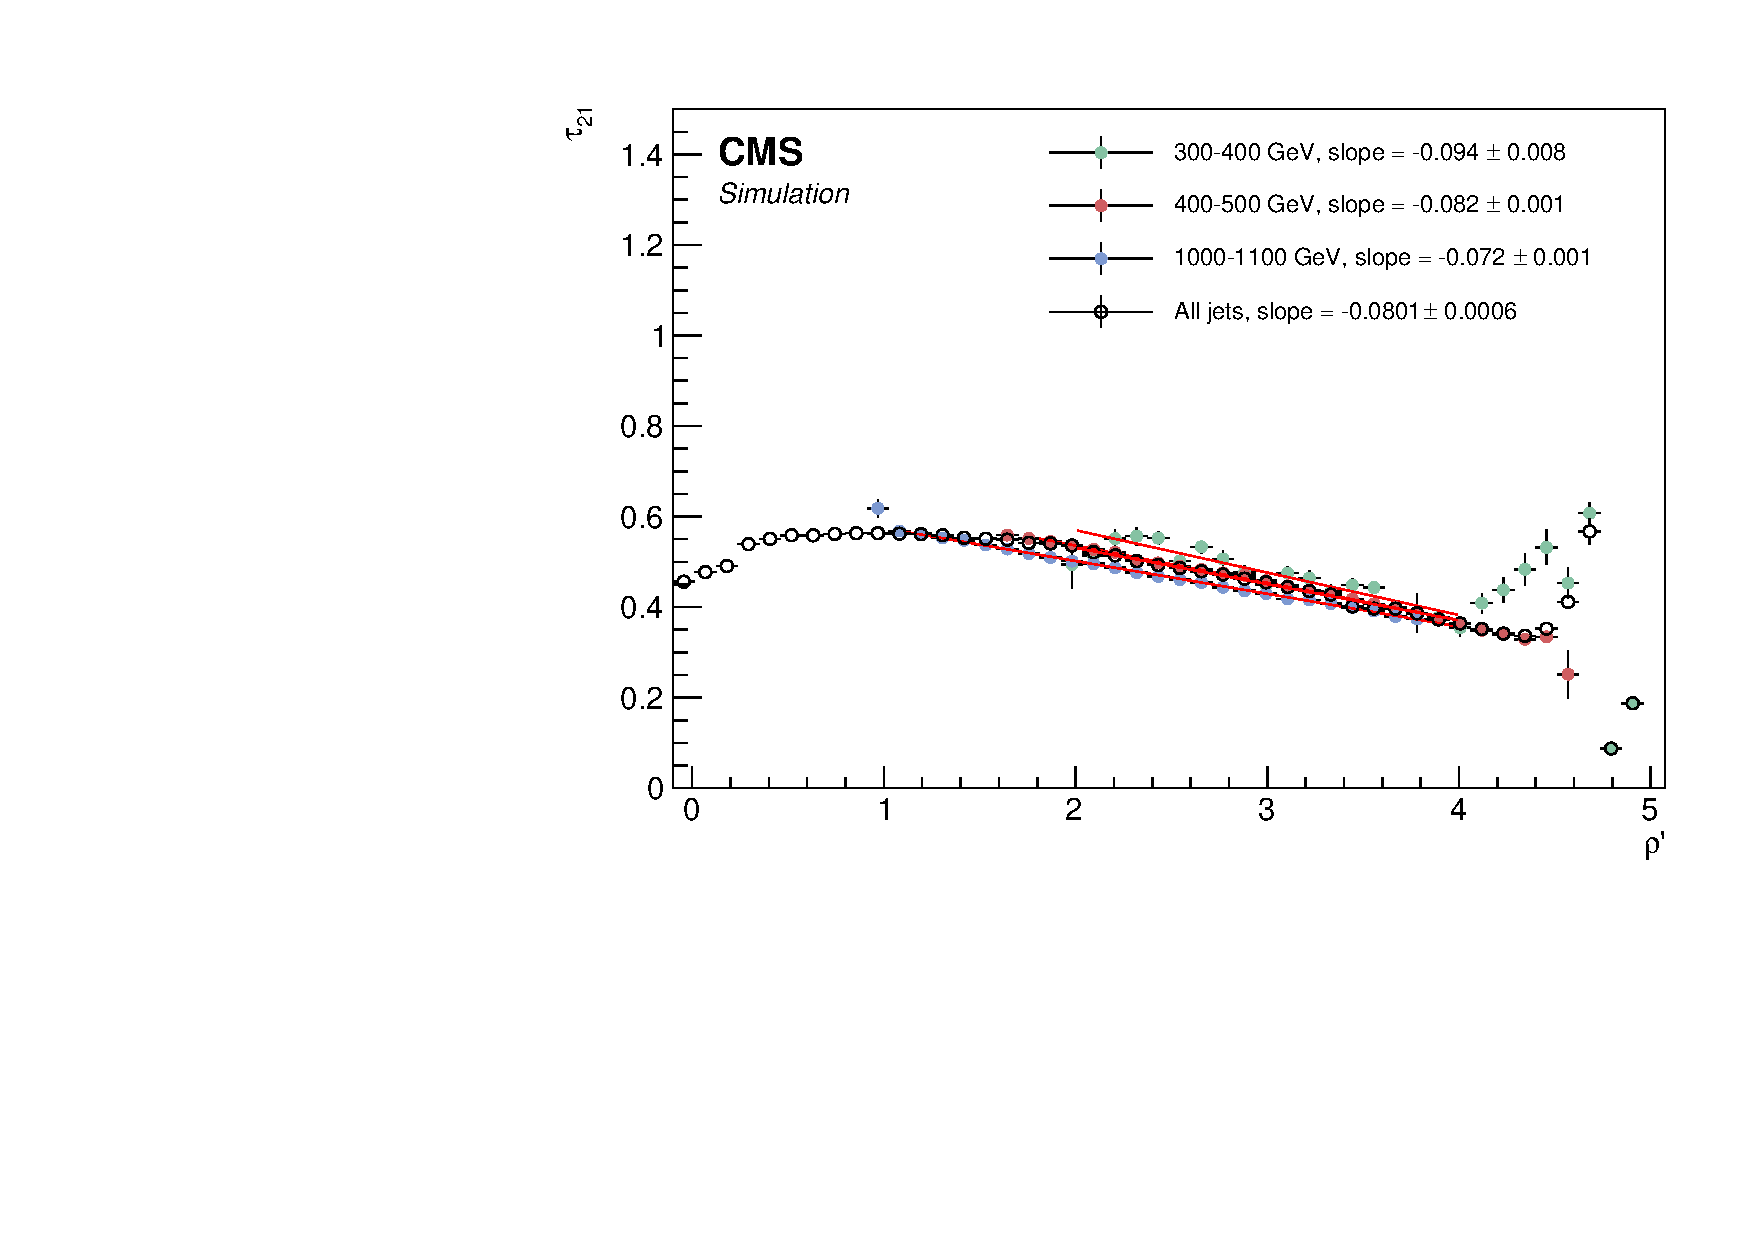
\includegraphics[width=0.45\textwidth]{figures/analysis/search3/AN-17-303/vtag/rho_pythia_FullSel_rhoPrime.pdf}\\
\end{tabular}
\caption{Profile distributions of $\tau_{21}$ as a function of $\rho' = log(m^2/p_T/\mu)$, where $\mu$ = 1 GeV (bottom), before applying a softdrop mass cut (left) and after applying a softdrop mass cut of $\unit{55}{\GeV} < \MJ < \unit{215}{\GeV}$ (right).}
\label{fig:rho}
\end{figure}
A linear transformation is then defined as
\begin{equation}
\label{eq:ddt}
\tau_{21}^{DDT}=\tau_{21}-M\times\rho',
\end{equation}
where the slope M is fitted from the linear part of the spectra of the $\tau_{21}$ profile versus $\rho'$ with full selections (bottom left plot). For our purposes, the slope is extracted from fitting the inclusive $p_T$-spectrum ("All jets") with a mass window applied
as it most closely corresponds to our full analysis selections. The resulting slope is $\ensuremath{M} = -0.080$, slightly steeper than than the 2016 value of $\ensuremath{M} = -0.063$~\cite{JME-16-003}.
The profile of the retuned $\tau_{21}^{DDT}$ versus $\rho'$ is shown in Figure~\ref{fig:rhoClosure}, exhibiting the desired flattened spectra.
\begin{figure}[htbp]
\centering
\begin{tabular}{cc}
% 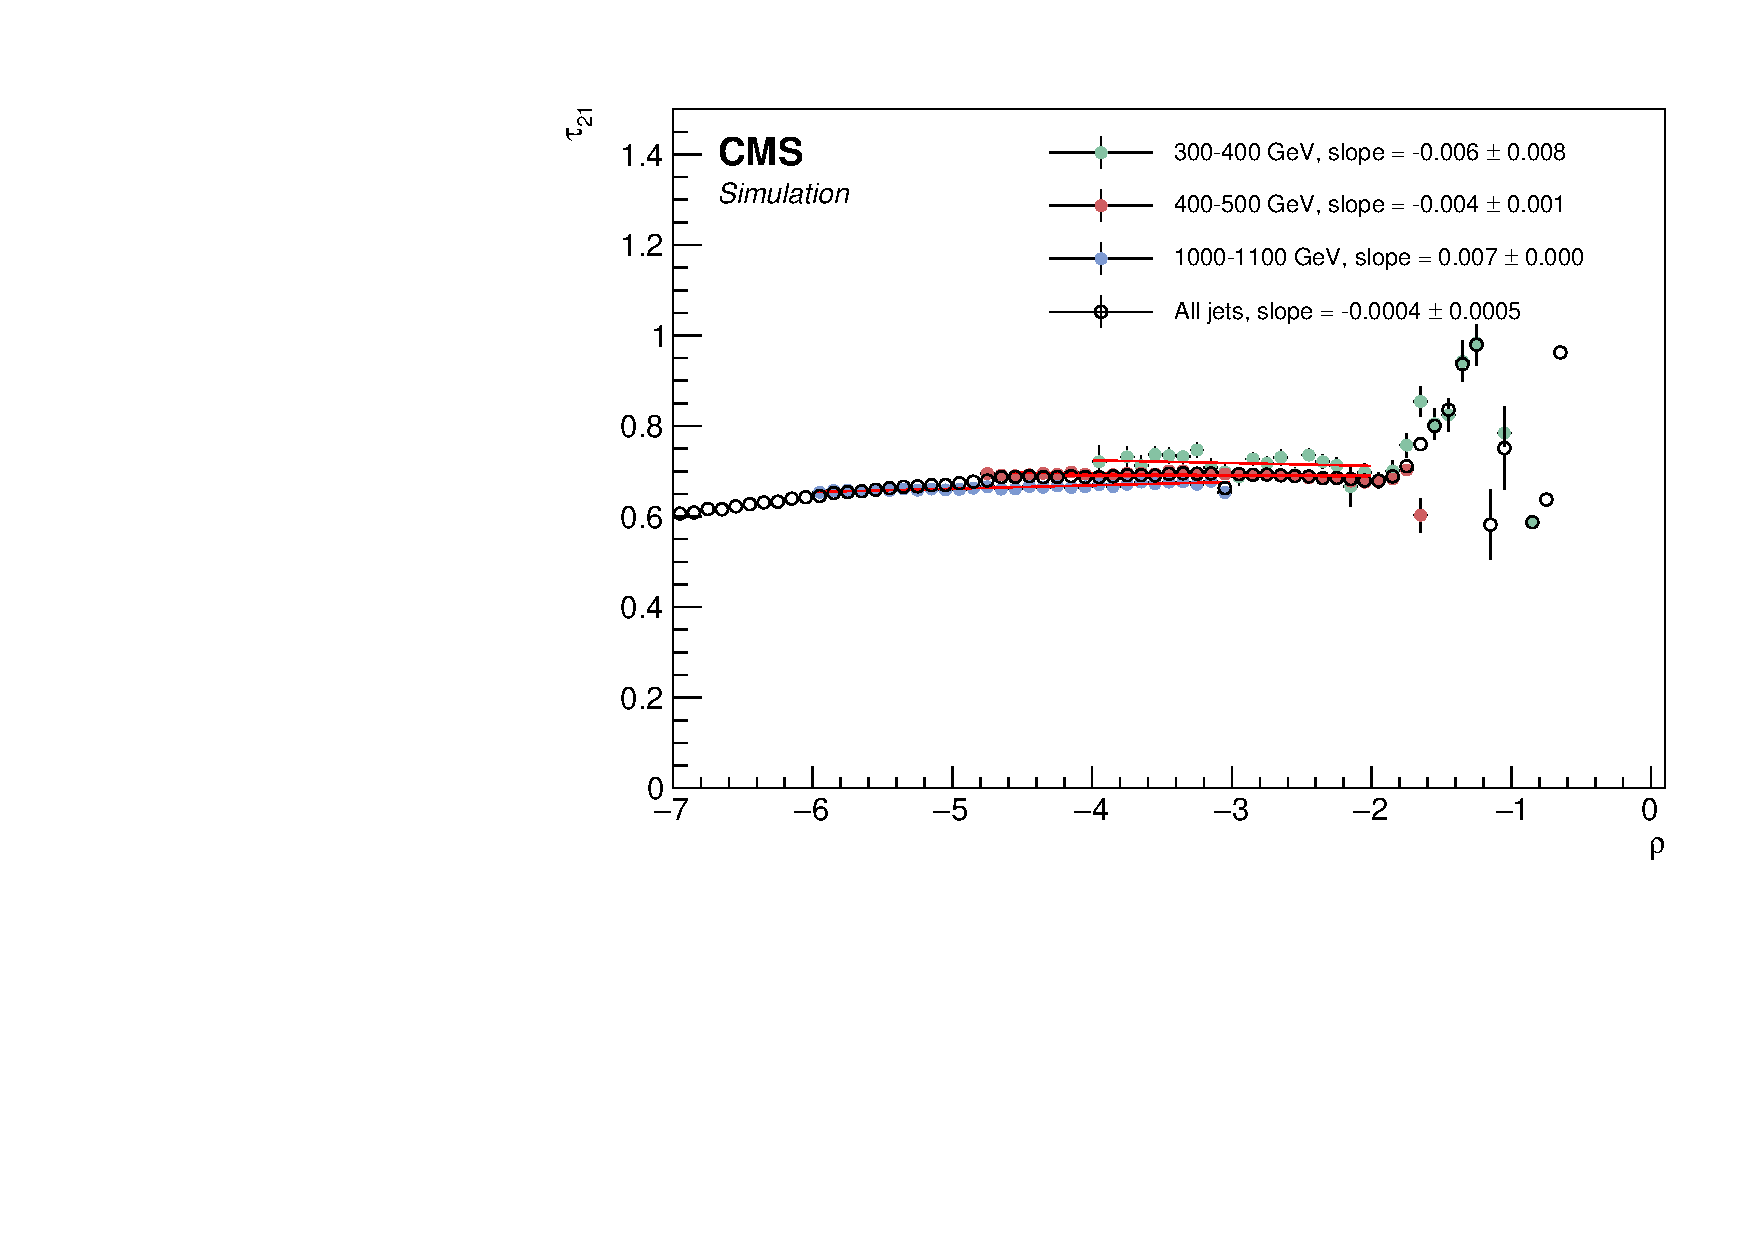
\includegraphics[width=0.45\textwidth]{figures/analysis/search3/AN-17-303/vtag/rho_pythia_FullSel_rhoClosure.pdf}
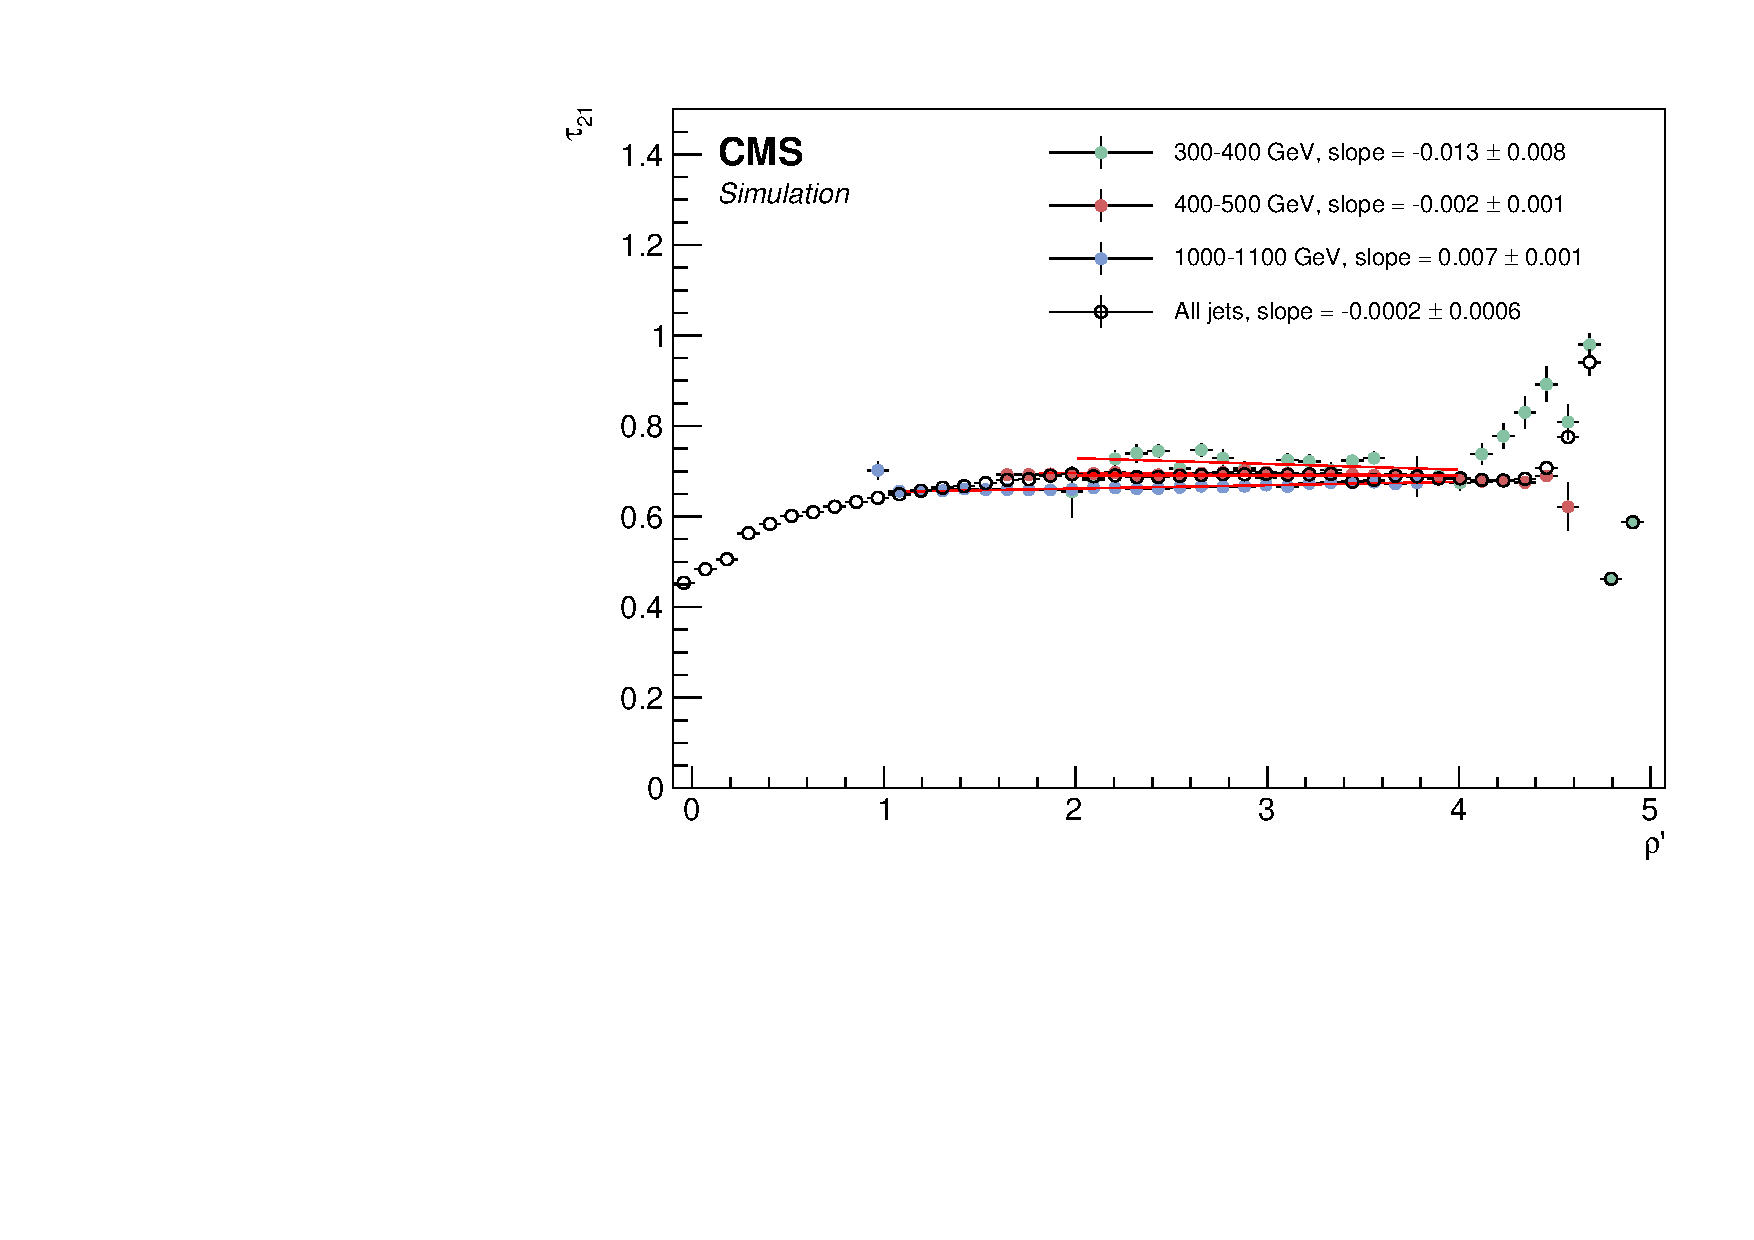
\includegraphics[width=0.45\textwidth]{figures/analysis/search3/AN-17-303/vtag/rho_pythia_FullSel_rhoPrimeClosure.pdf}
\end{tabular}
\caption{Profile distributions of $\tau_{21}^{DDT}$ as a function of $\rho' = log(m^2/p_T/\mu)$, where $\mu$ = 1 GeV.}
\label{fig:rhoClosure}
\end{figure}
Working points for $\tau_{21}^{DDT}$ are chosen in the following way: First, we check which $\tau_{21}^{DDT}$ cut corresponds to the highest Punzi significance as a function of the resonance mass for different signal samples, shown in Figure~\ref{fig:punzi}. All other analysis cuts cuts have been applied.
\begin{figure}[htbp]
\centering
\begin{tabular}{cc}
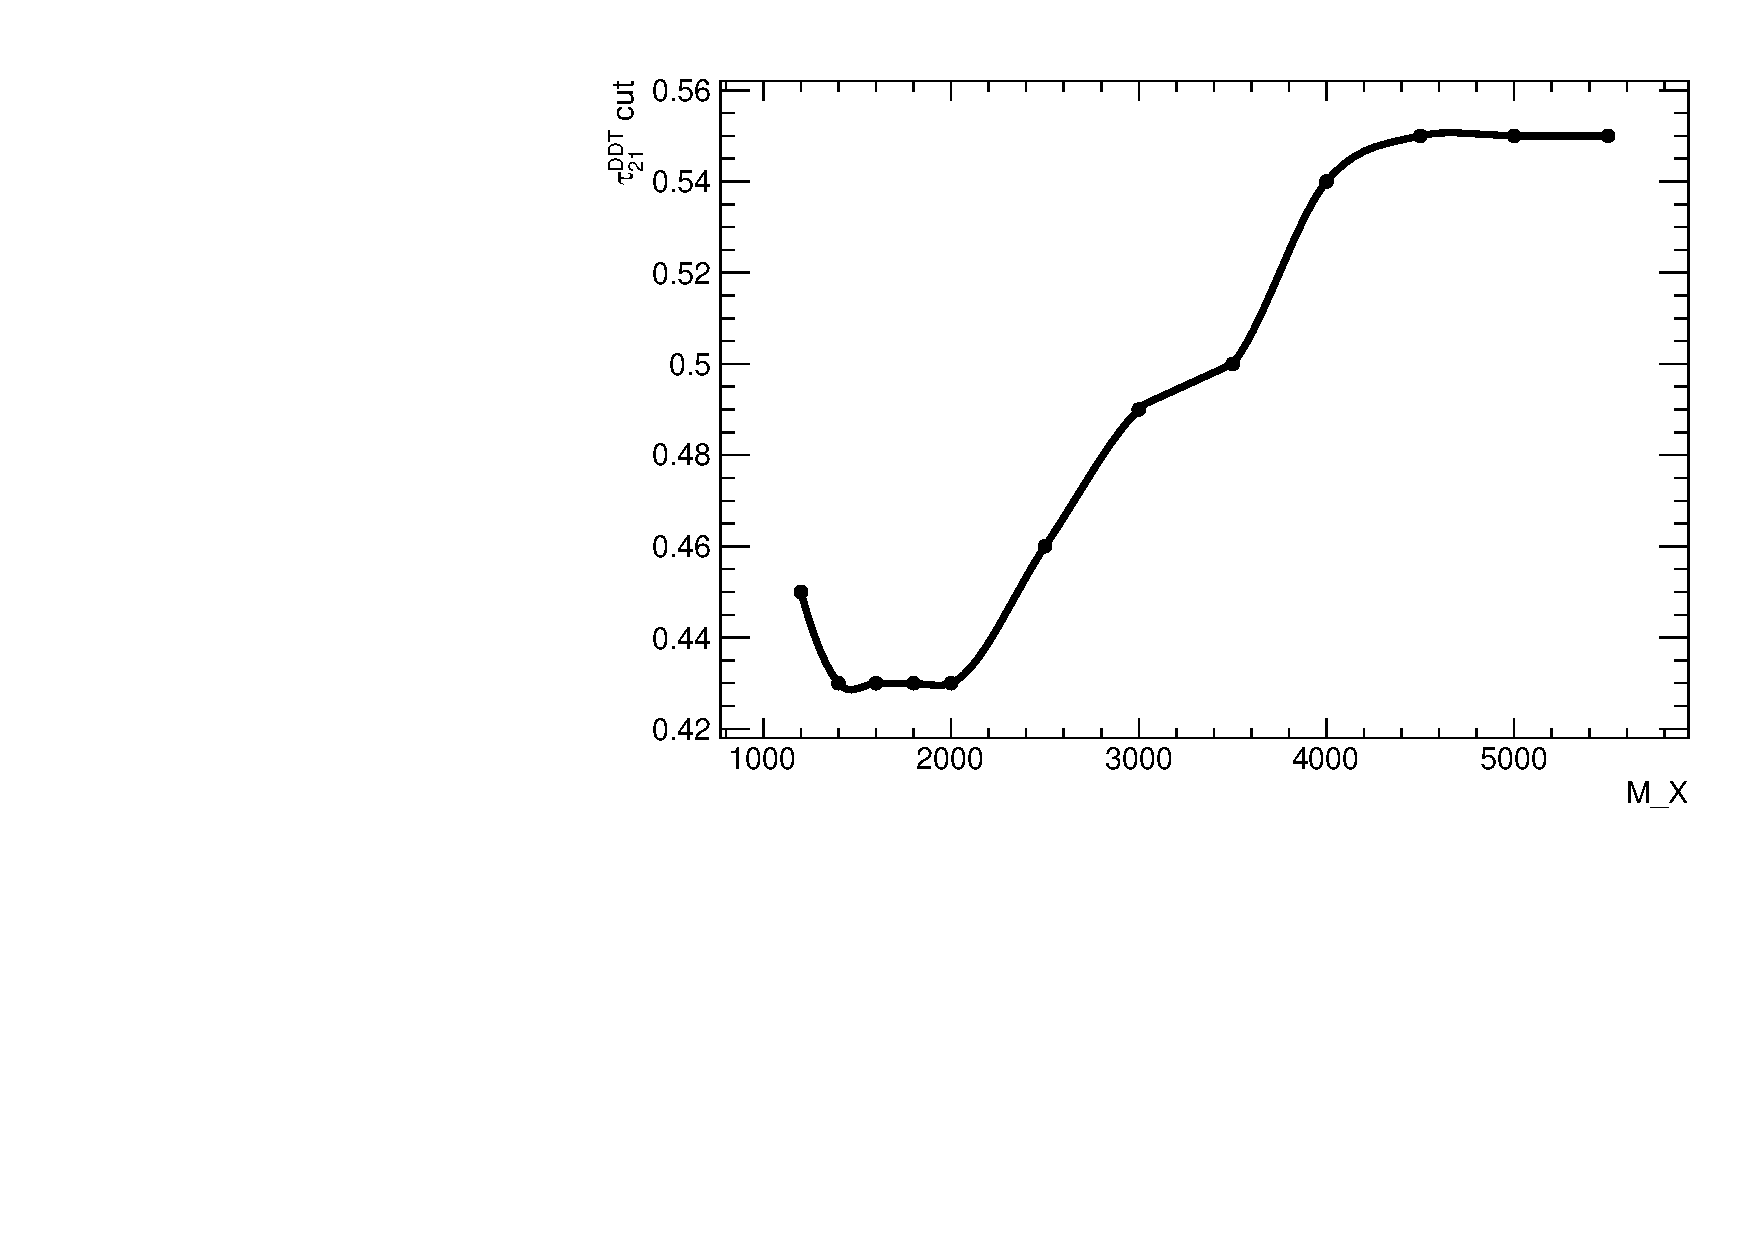
\includegraphics[width=0.45\textwidth]{figures/analysis/search3/AN-17-303/vtag/tau21ddt_punzi_BulkGravToZZToZhadZhad.pdf}
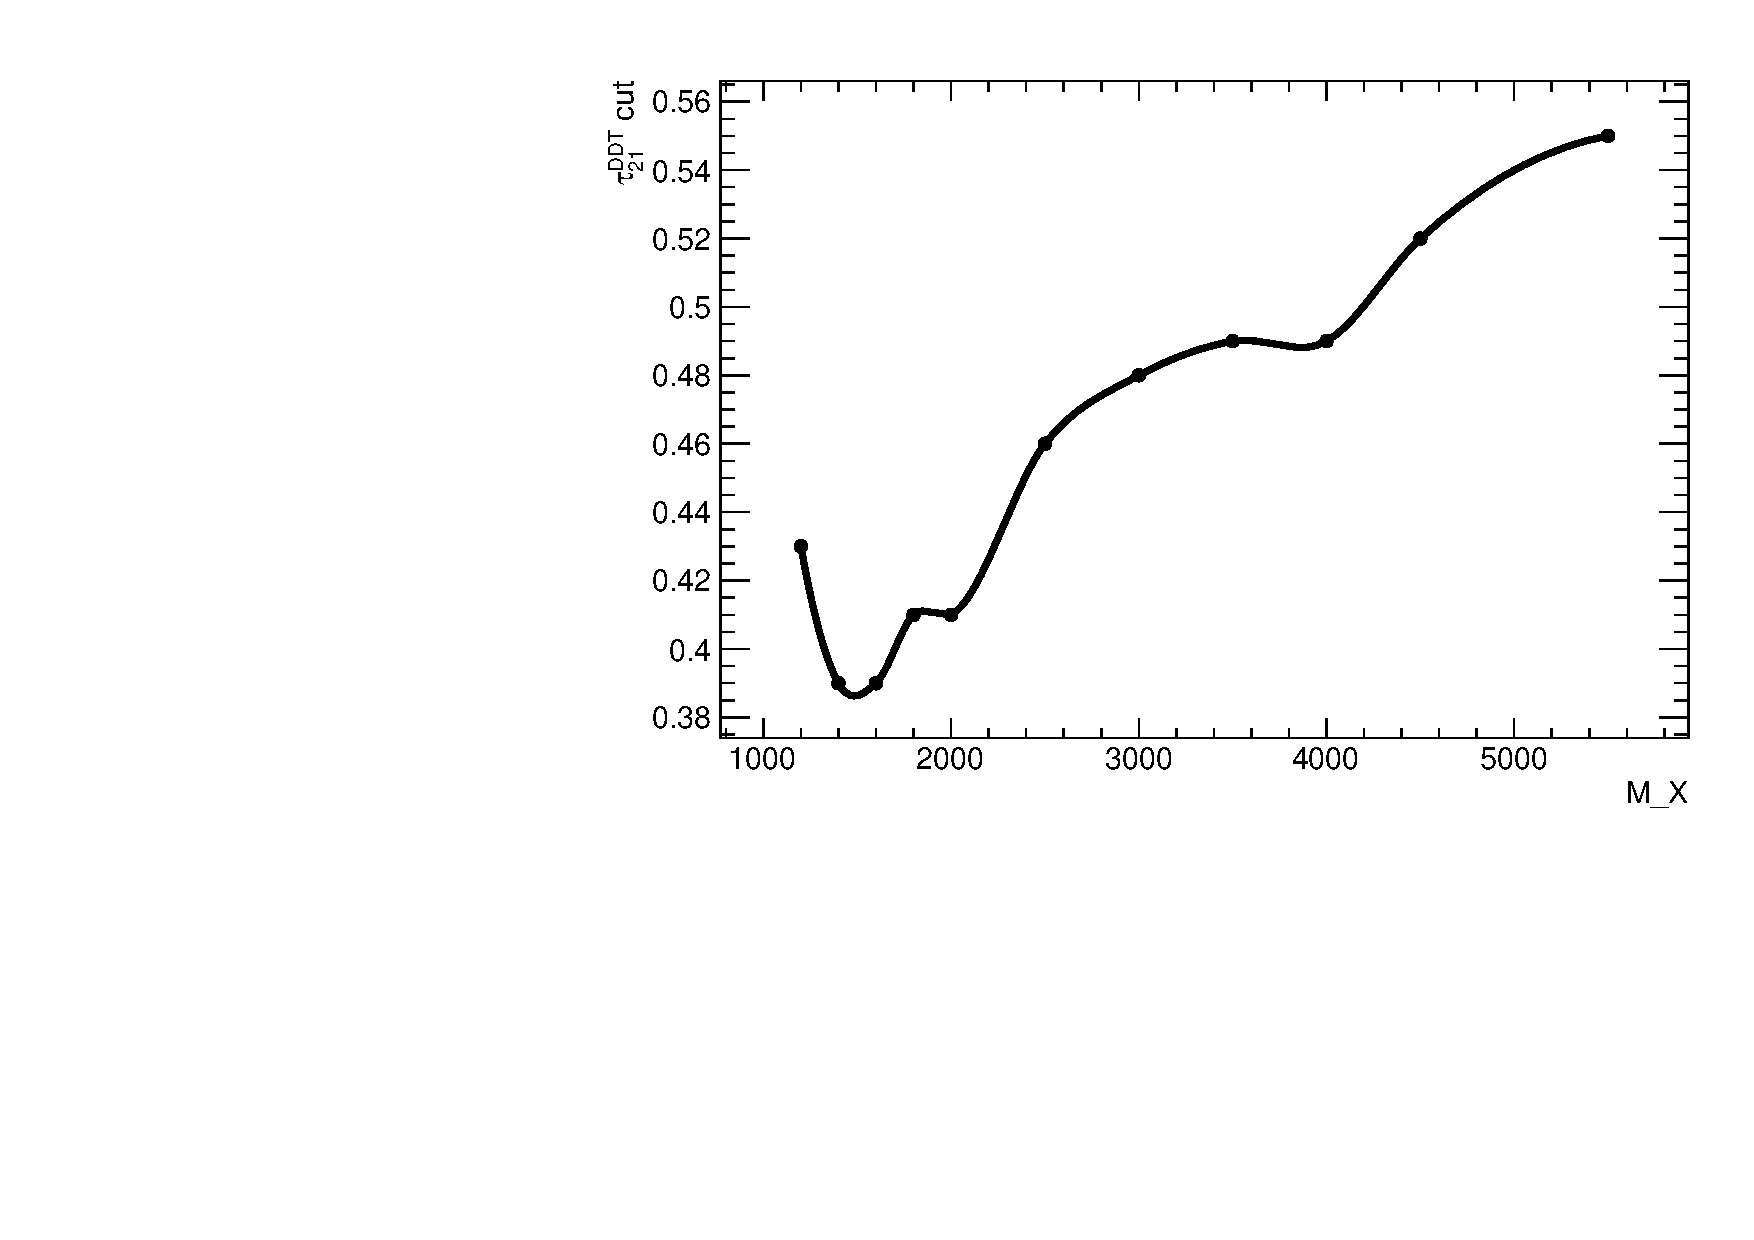
\includegraphics[width=0.45\textwidth]{figures/analysis/search3/AN-17-303/vtag/tau21ddt_punzi_BulkGravToWW.pdf}
\end{tabular}
\caption{The $\tau_{21}^{DDT}$ cut corresponding to the highest Punzi significance for a given signal resonance mass, here for Bulk $G\rightarrow WW$ (left) and Bulk $G\rightarrow ZZ$.}
\label{fig:punzi}
\end{figure}
The cut maximizing the Punzi significance at low resonance mass, where the background is highest, is chosen as the "high purity" (HP) working point.
This corresponds to $\tau_{21}^{DDT} \leq 0.43$
Second, we find the cut which, together with events falling in the HP region, contains at least 95 percent of the signal as well as optimizes the Punzi significance. This is found to be $0.43<\tau_{21}^{DDT}\leq0.79$, and is classified as the low purity (LP) category. The purpose of this category is to enhance the overall sensitivity, especially where the background is low.
We observe a significant gain in signal efficiency at a fixed mistag rate with the retuned DDT tagger. The signal efficiency versus mistagging rate for all three taggers is shown in Figure~\ref{fig:roc}, and we see the retuned \ddt performing better than \nsubj and the version of \ddt using the old tune.
\begin{figure}[htbp]
\centering
\begin{tabular}{cc}
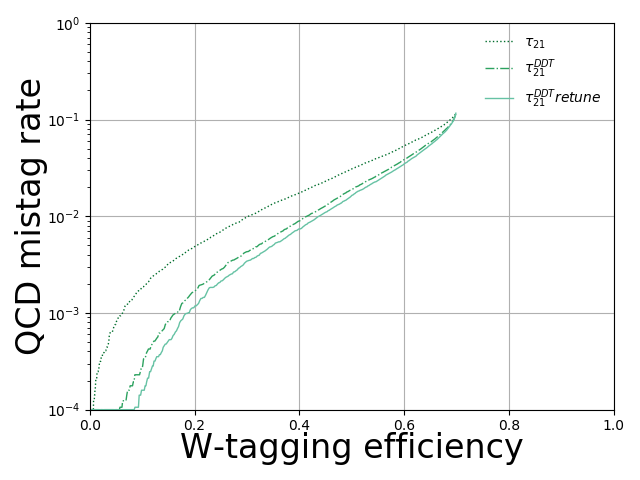
\includegraphics[width=0.49\textwidth]{figures/analysis/search3/AN-17-303/vtag/LoLa-comp-roc-simple.png}
\end{tabular}
\caption{Performance of $\tau_{21}$ and $\tau_{21}^{DDT}$ (2016 and 2017 tune) in the background-signal efficiency plane.}
\label{fig:roc}
\end{figure}
In addition to cutting on $\tau_{21}^{DDT}$ a loose cut of $\rho = log(m^2/p_T^2) < -1.8 $ is applied.
The reason for this is that, while the distribution of $\rho$ is flat as a function of jet transverse momentum for QCD jets, this only holds in the region where perturbative contributions dominate and breaks down at around $\rho = log(m^2/p_T^2) < -2.0$ due to the AK8 cone size being to small to contain the full jet at high masses. This has a negligible effect on the signal, which
mainly peaks around 80 GeV and has a relatively high jet transverse momenta.
Figure~\ref{fig:wtagCP} shows the signal and background distribution for the PUPPI softdrop jet mass and \ddt. The signal softdrop mass distribution peaks nicely around the W mass, while the multijets background spectrum is peaked at lower softdrop masses. Also, in addition to having a higher signal efficiency for a given mistag rate, $\tau_{21}^{DDT}$ has the added benefit of being better modeled in MC than $\tau_{21}$.
\begin{figure}[htbp]
\centering
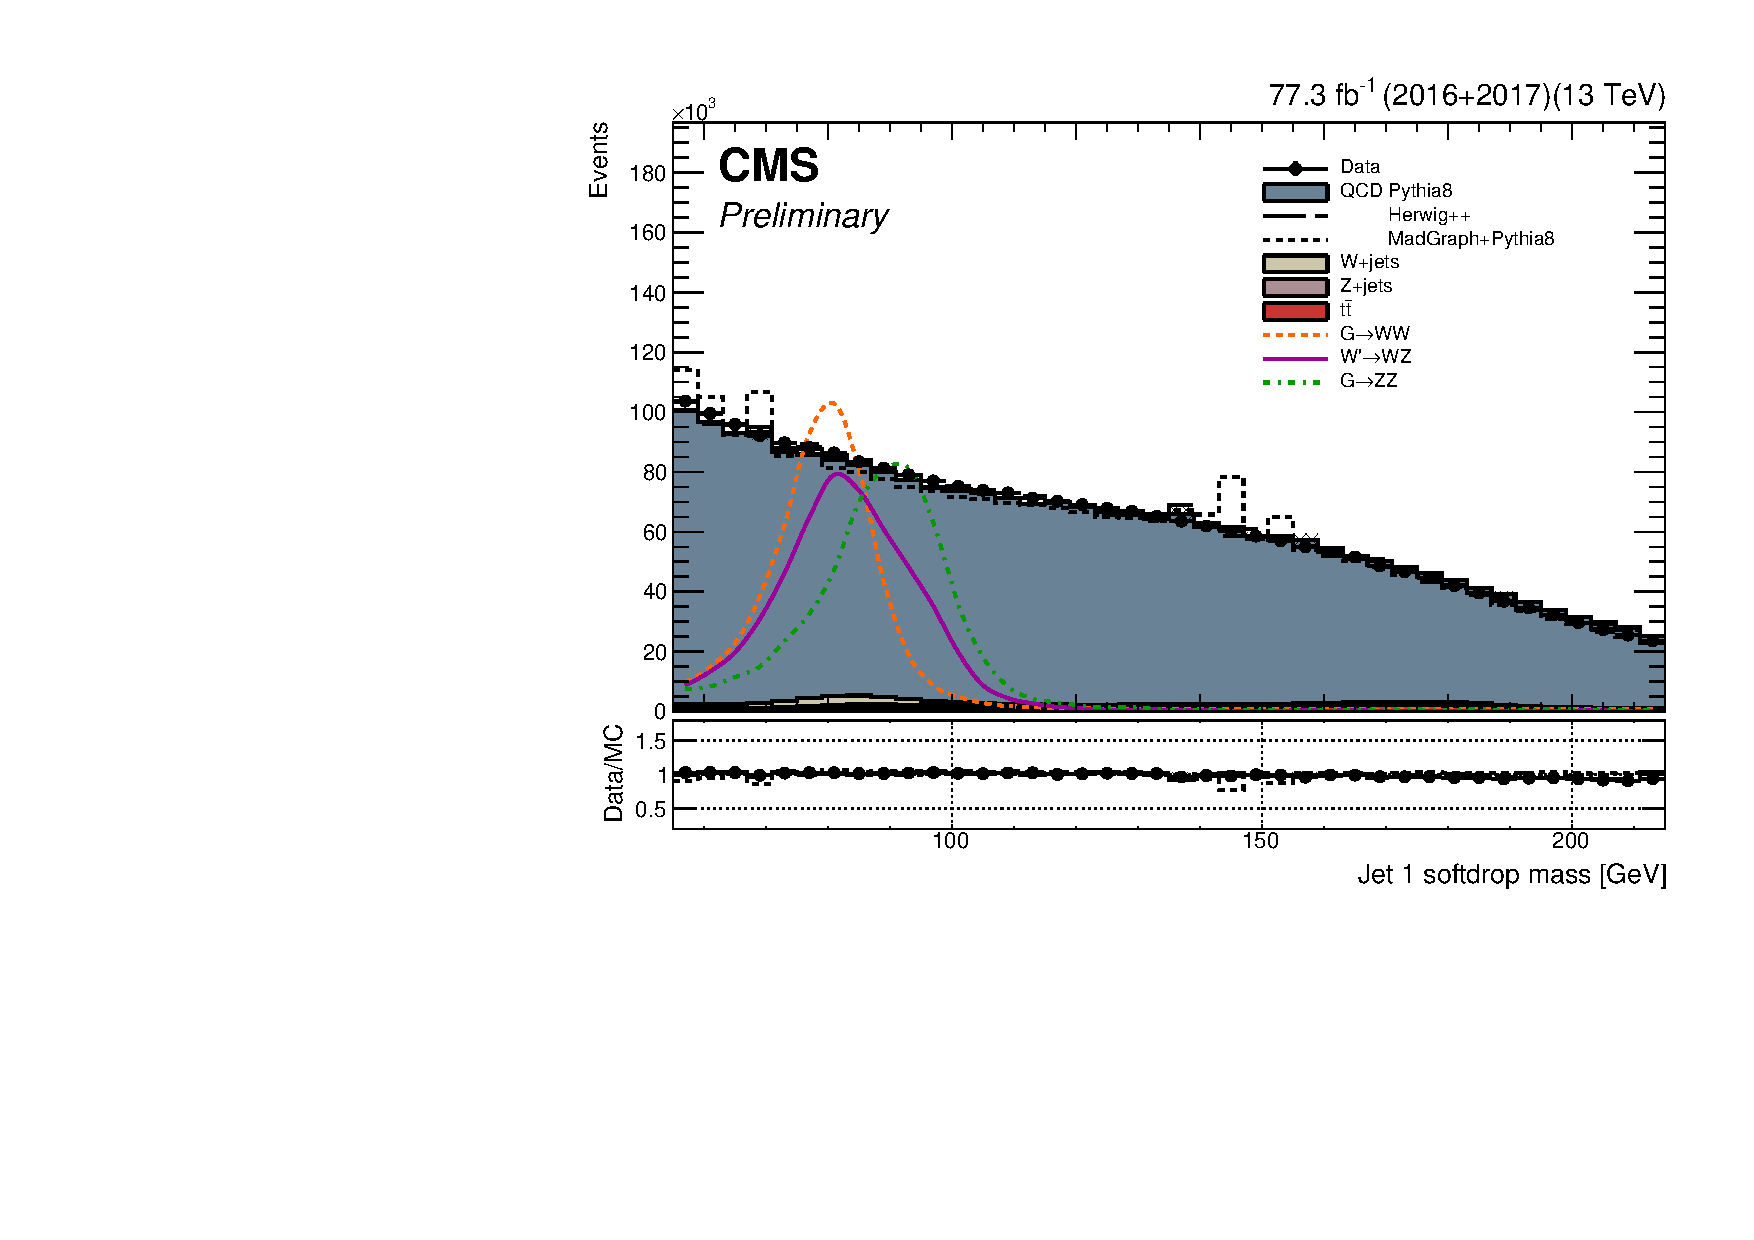
\includegraphics[width=0.450\textwidth]{figures/analysis/search3/B2G-18-002/looseSel_Jet_1_softdrop_mass.pdf}
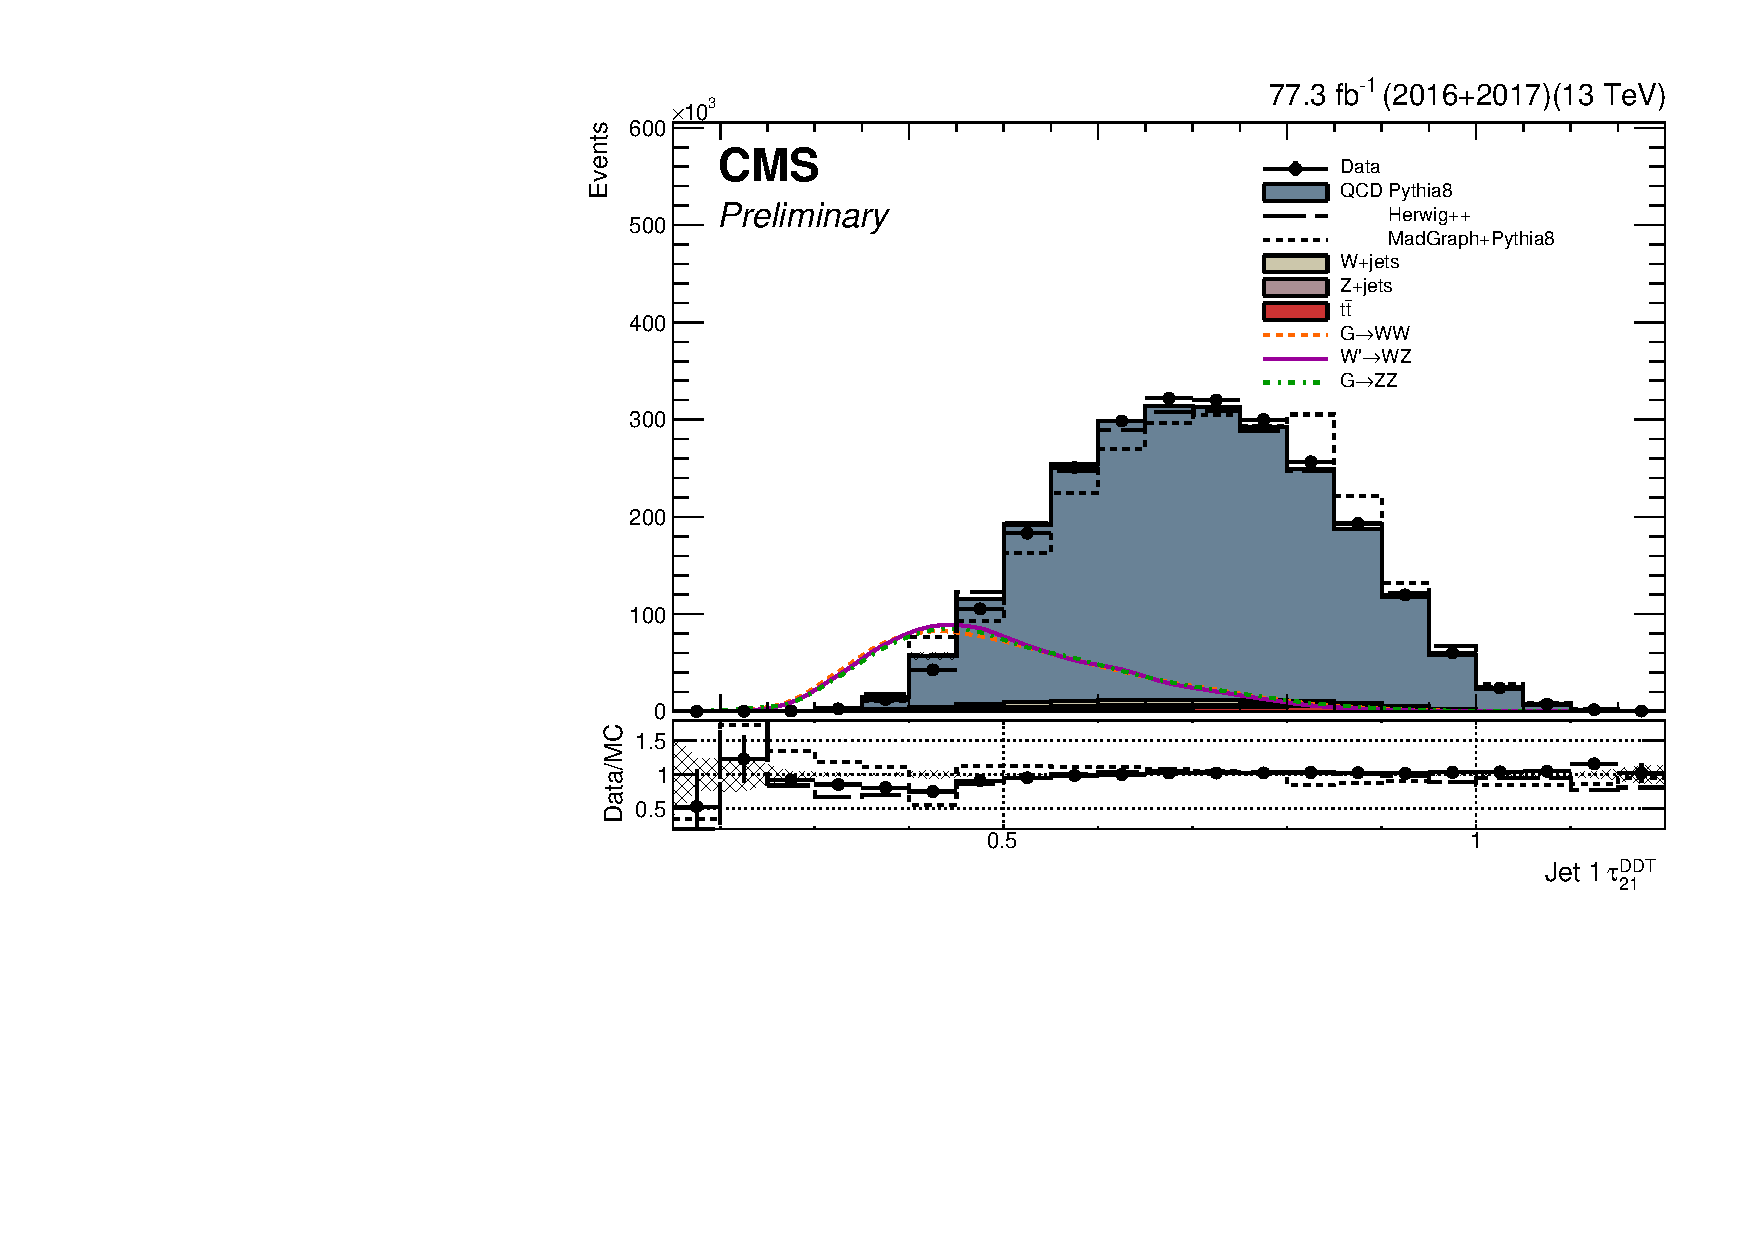
\includegraphics[width=0.450\textwidth]{figures/analysis/search3/B2G-18-002/looseSel_Jet_1_DDT.pdf}\\
\caption{PUPPI softdrop jet mass distribution (left) and PUPPI N-subjettiness $\tau_{21}^{DDT}$ (right). Signal is scaled with an arbitrary number.}
\label{fig:wtagCP}
\end{figure}
\clearpage
\subsubsection{Data to simulation scale factors}
\label{sec:searchIII:wtagSF}
Following what was done in Section~\ref{sec:searchI:vtag} and~\ref{sec:searchII:wtagsf}, we derive W-tagging scale factors for the efficiency of the selection on $\tau_{21}^{DDT}$ by estimating the ratio of the selection efficiencies on data and simulation. The PUPPI softdrop mass range is extended to 55 to 215 \GeV, and the two purity categories are
\begin{itemize}
\itemsep0em
  \item Pass region: $0 <  \ddt \leq 0.43 \sim$ high purity
  \item Fail region: $0.43 < \nsubj \leq 0.79 \sim$ low purity
\end{itemize}
The obtained scale factors are listed in Tables~\ref{tab:wsf16} and~\ref{tab:wsf} for 2016 and 2017 data, respectively, with the corresponding simultaneous fits shown in Fig.~\ref{fig:simFit}. 
The jet mass scale and resolution together with their are estimated in the same fits and also listed in Table~\ref{tab:wsf}. Two additional uncertainties are added: one due to generator differences and one due to NNLO corrections. These are evaluated by comparing the extracted efficiency with and without top \PT reweighting and when using \ttbar simulation produced with different generators. The scale factors, jet mass scale and jet mass resolution with their total uncertainty after adding systematics, are listed in Table~\ref{tab:wsf_total}. As before, the scale factor is added as a scale of the the signal yield and the jet mass scale and resolution are used to smear MC, and are additionally inserted as systematic uncertainties in the final fit (scale up/down).
 \begin{table}[htbp]
    \centering
    \begin{tabular}{|lccc|}
    \hline
    & m [GeV]           & $\sigma$~[GeV]     & W-tag efficiency\\
    $\tau_{21}^{DDT} < 0.43$ & &&\\ \hline
    \hline
    Data            & 81.999$\pm$ 0.454~GeV   & 7.148 $\pm$ 0.544~GeV & 0.080 $\pm$ 0.008\\
    Simulation      & 80.890$\pm$ 0.160~GeV   & 6.579 $\pm$ 0.149~GeV & 0.085 $\pm$ 0.003\\
    \hline
    Data/simulation & 1.014$\pm$ 0.006       & 1.086 $\pm$ 0.086     & 0.937 $\pm$ 0.094\\
    \hline
    $0.43 < \tau_{21}^{DDT} < 0.79$ & &&\\ \hline
    \hline
    Data            &    &  & 0.920 $\pm$ 0.008\\
    Simulation      &    &  & 0.915 $\pm$ 0.003\\
    \hline
    Data/simulation &    &   & 1.006 $\pm$ 0.009\\
    \hline
    \end{tabular}
     \caption{Jet mass scale, jet mass resolution and $\tau_{21}^{DDT}$ scale factors as evaluated in the full 2016 Single Muon dataset.}
    \label{tab:wsf16}
 \end{table}
 \begin{table}[htbp]
    \centering
    \begin{tabular}{|lccc|}
    \hline
    & m [GeV]           & $\sigma$~[GeV]     & W-tag efficiency\\
    $\tau_{21}^{DDT} < 0.43$ & &&\\ \hline
    \hline
    Data            & 80.784$\pm$ 0.391~GeV   & 7.694 $\pm$ 0.445~GeV & 0.065 $\pm$ 0.006\\
    Simulation      & 82.208$\pm$ 0.293~GeV   & 7.127 $\pm$ 0.284~GeV & 0.068 $\pm$ 0.005\\
    \hline
    Data/simulation & 0.983$\pm$ 0.006       & 1.080 $\pm$ 0.076     & 0.955 $\pm$ 0.113\\
    \hline
    $0.43 < \tau_{21}^{DDT} < 0.79$ & &&\\ \hline
    \hline
    Data            &    &  & 0.935 $\pm$ 0.006\\
    Simulation      &    &  & 0.932 $\pm$ 0.005\\
    \hline
    Data/simulation &    &   & 1.003 $\pm$ 0.008\\
    \hline
    \end{tabular}
    \caption{Jet mass scale, jet mass resolution and $\tau_{21}^{DDT}$ scalefactors as evaluated in the full 2017 Single Muon dataset.}
    \label{tab:wsf}
 \end{table}
 \begin{figure}[htbp]
 \centering
 \begin{tabular}{cc}
 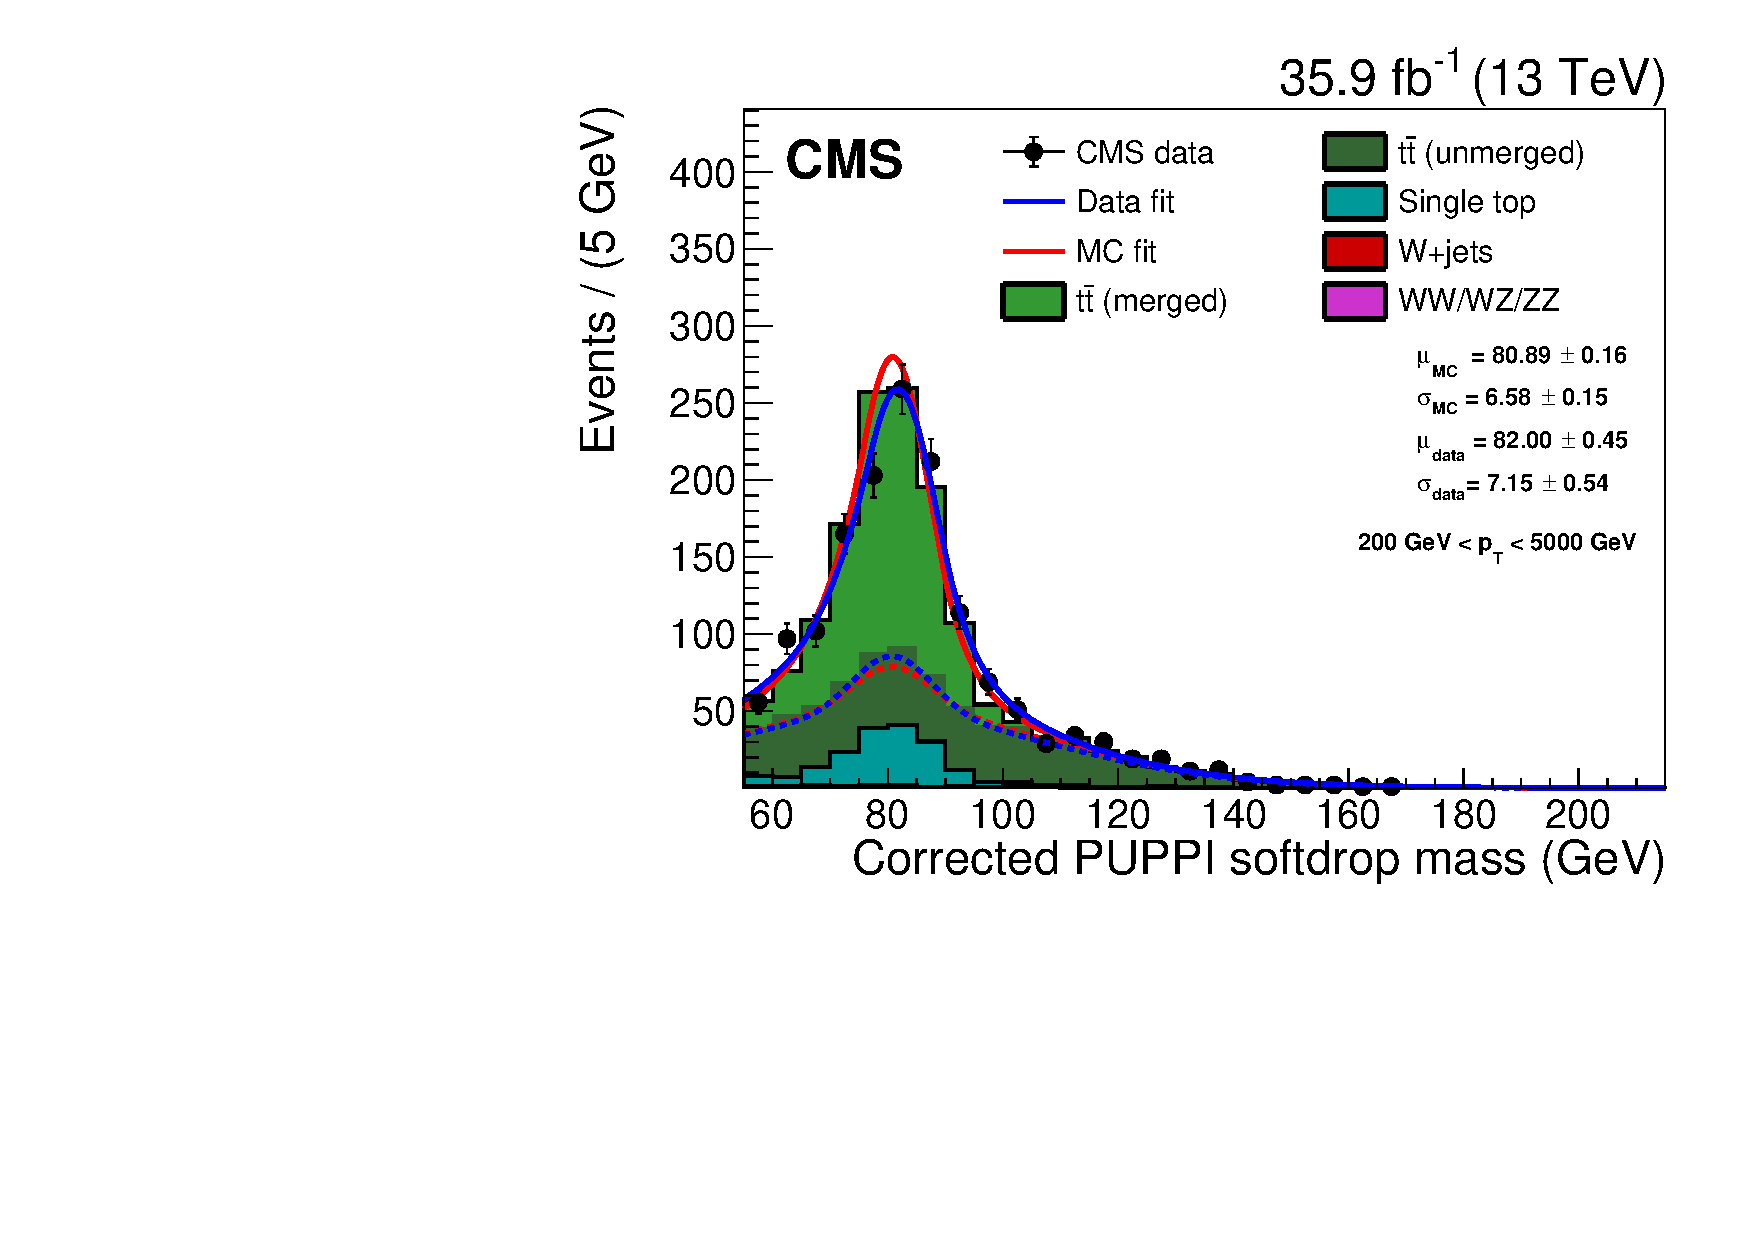
\includegraphics[width=0.49\textwidth]{figures/analysis/search3/AN-17-303/vtag/newddt_2016_pass.pdf}
 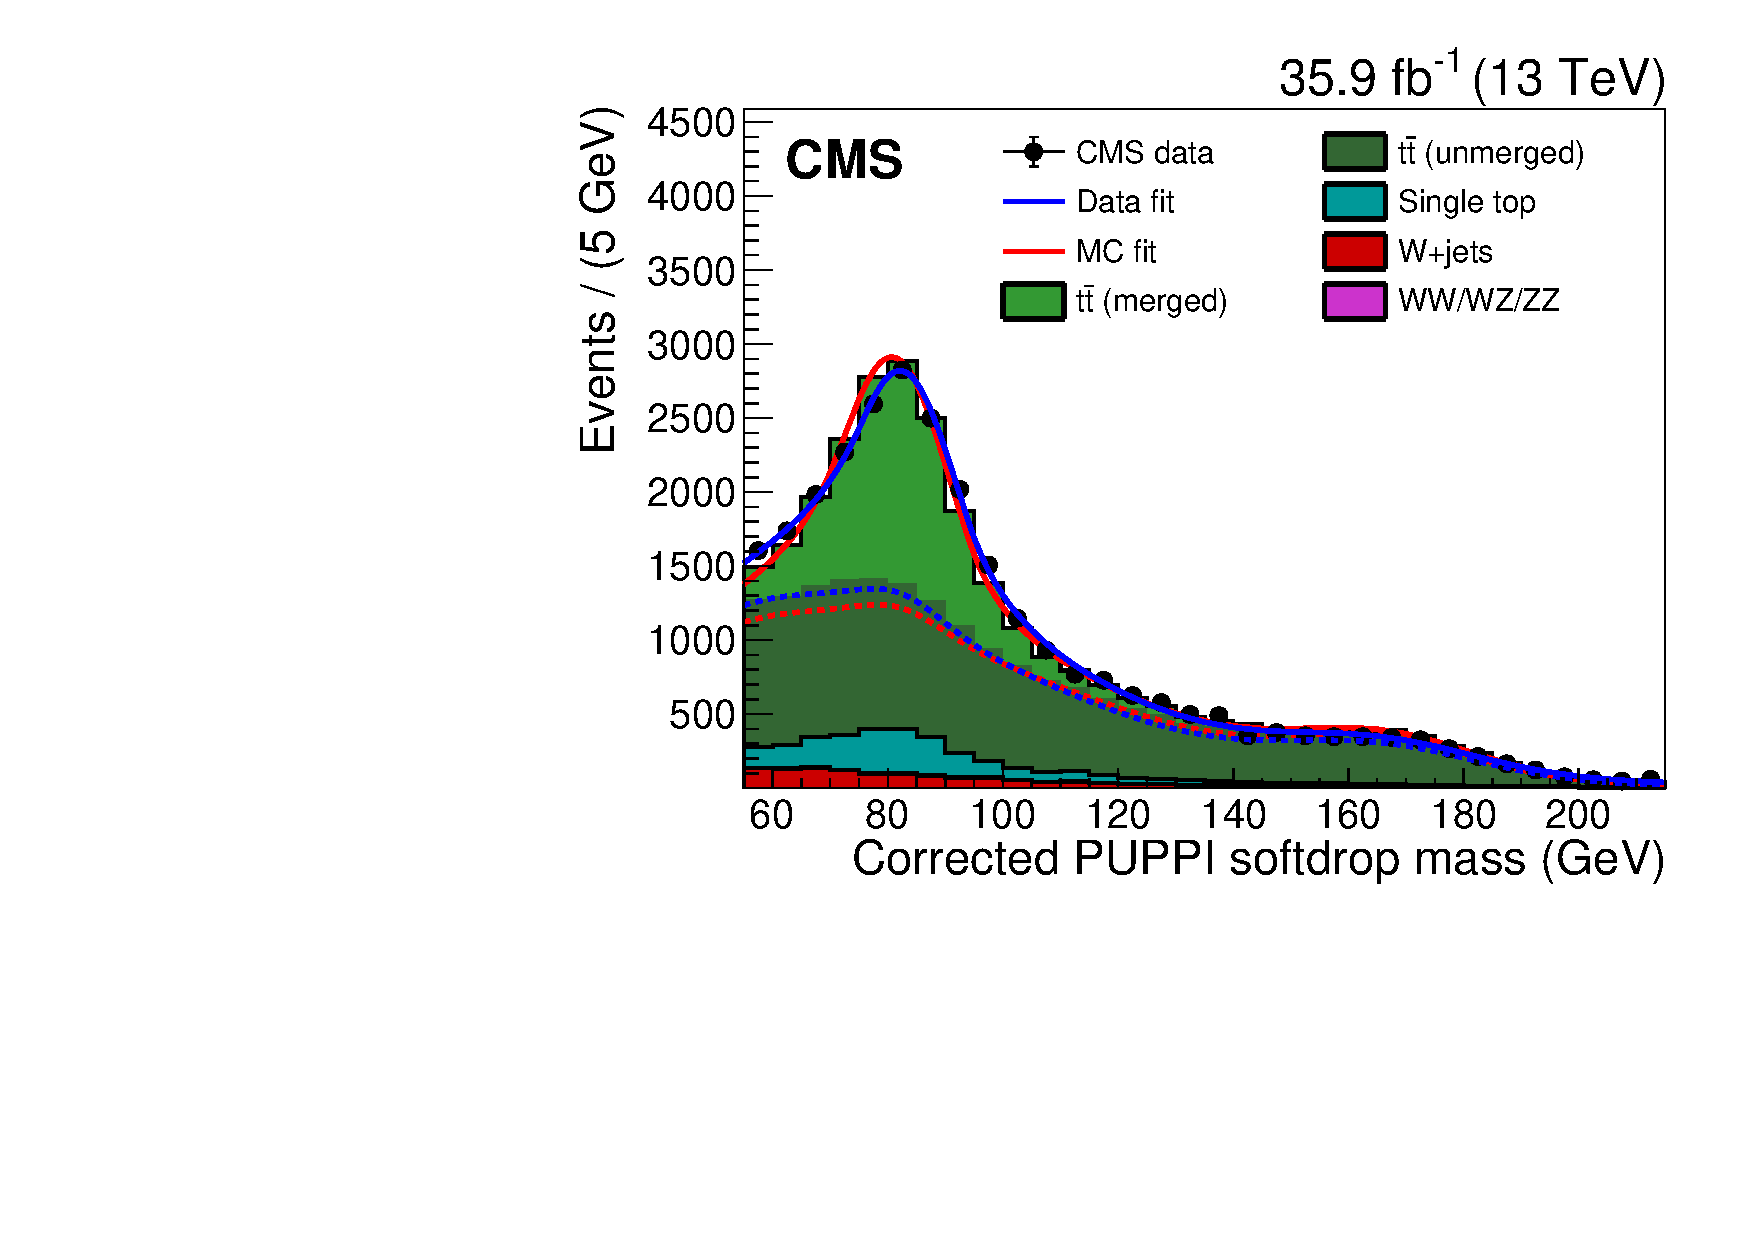
\includegraphics[width=0.49\textwidth]{figures/analysis/search3/AN-17-303/vtag/newddt_2016_fail.pdf}\\
 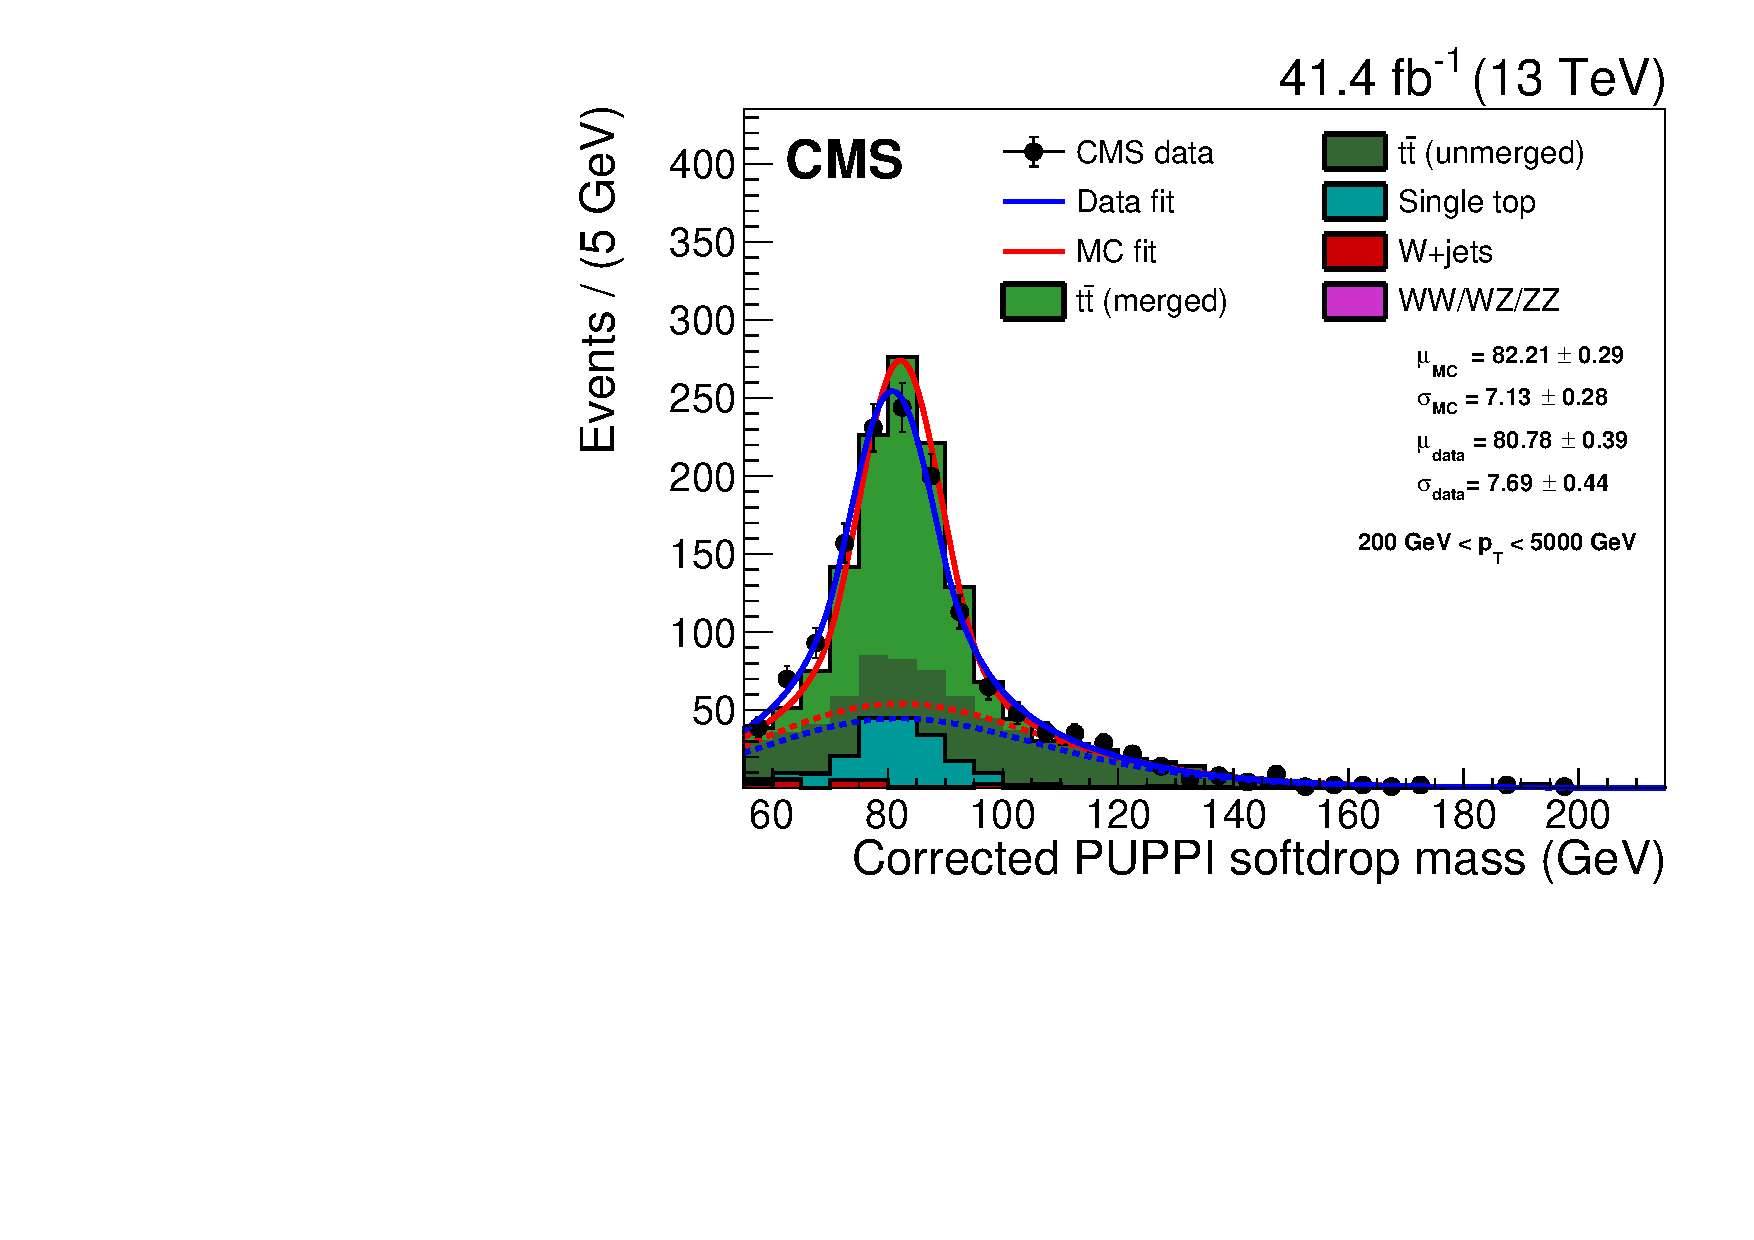
\includegraphics[width=0.49\textwidth]{figures/analysis/search3/AN-17-303/vtag/newddt_TopPtRew_2017_pass.pdf}
 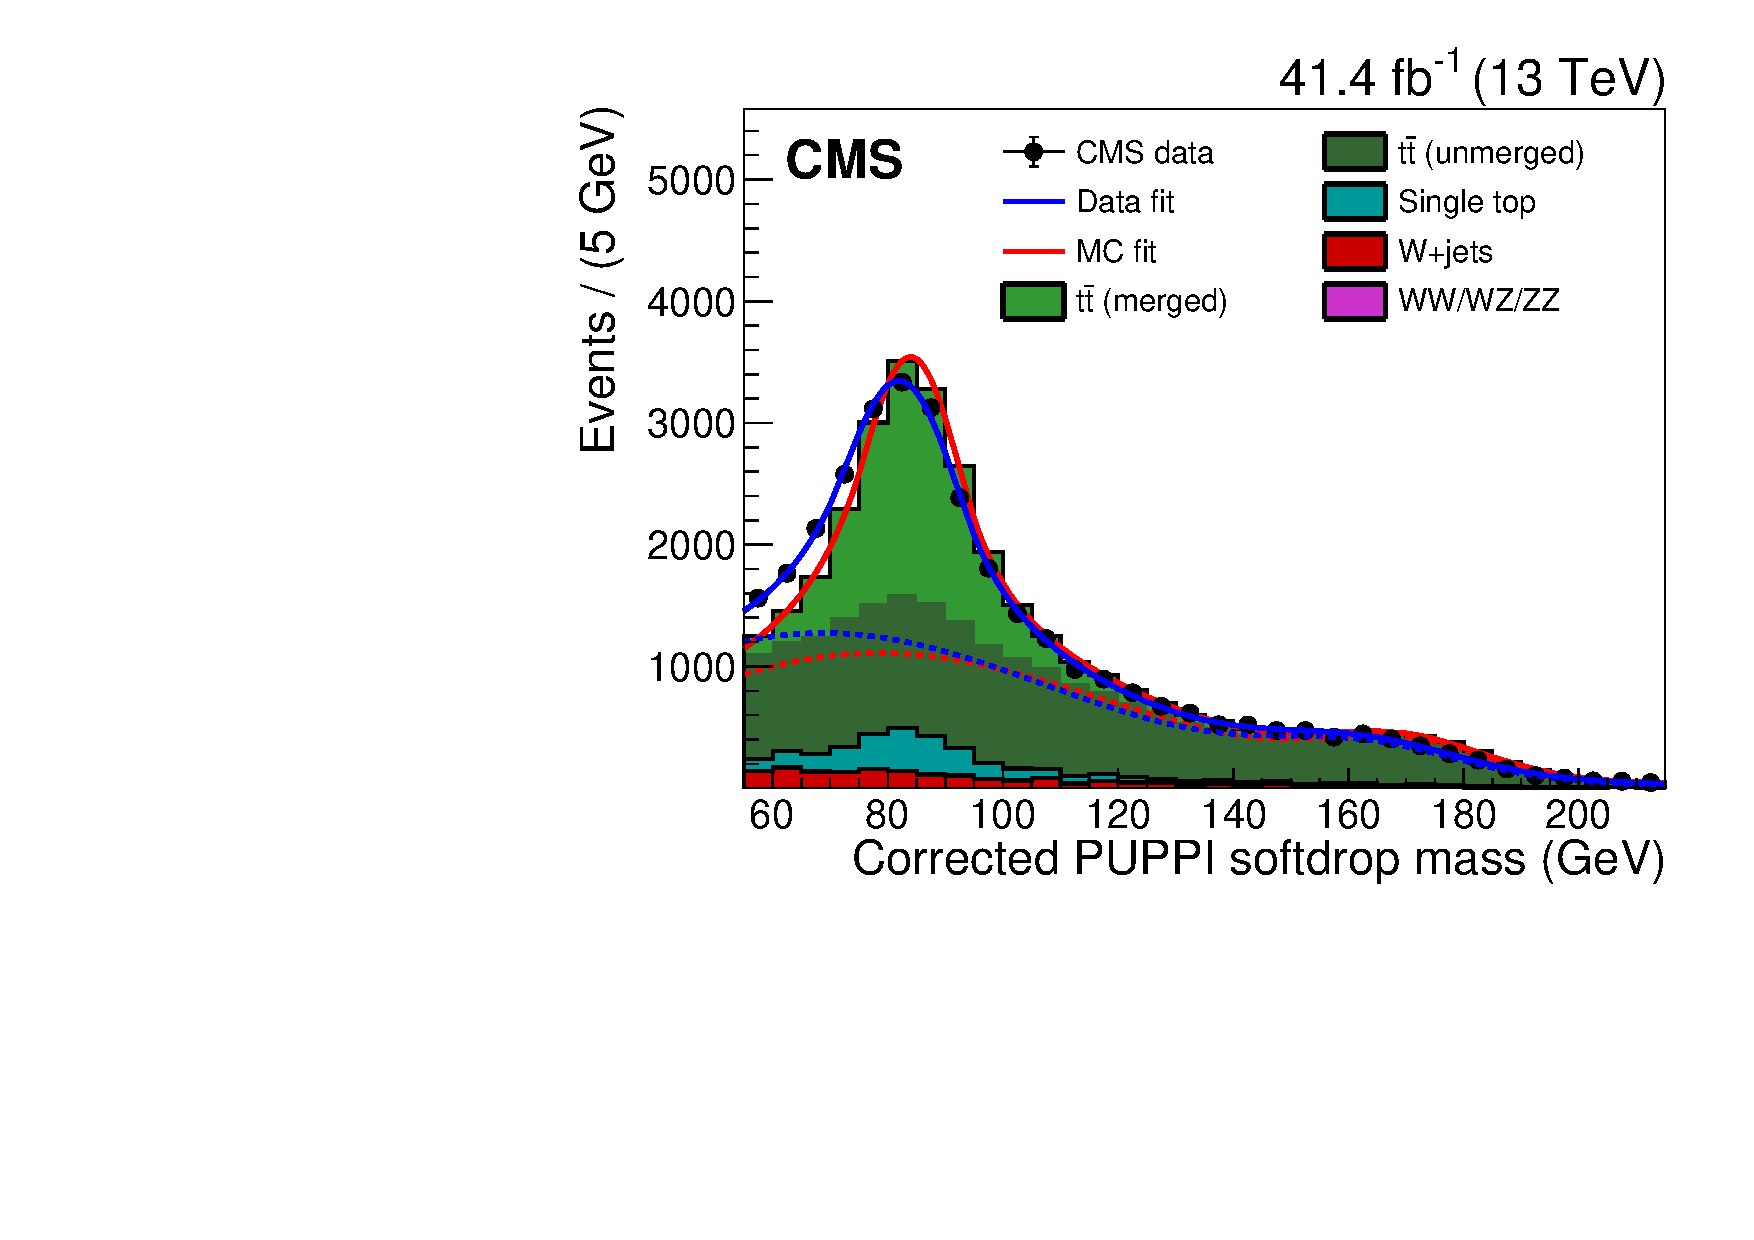
\includegraphics[width=0.49\textwidth]{figures/analysis/search3/AN-17-303/vtag/newddt_TopPtRew_2017_fail.pdf}
 \end{tabular}
 \caption{PUPPI softdrop jet mass distribution that pass (left) and fail (right) the \ddt 0.43 selection in the \ttbar control sample. The result of the fit to data and simulation are shown by the solid blue and solid red line, respectively. The background components of the fit are shown as dashed-dotted lines. The fit to 2016 data is shown in the upper panels and the fit to 2017 data in the lower panels.}
 \label{fig:simFit}
 \end{figure}
 \begin{table}[htbp]
    \centering
     \begin{tabular}{|l|c|c|}
     \hline
      & SF $\pm \sqrt{\textrm{Stat.} \pm \textrm{Sys}_{\rm{Generator}} \pm \textrm{Sys}_{\rm{NNLO}}}$ & SF $\pm$ Total Unc. \\
    \hline
    $HPSF_{DDT}^{2017}$ &  $0.955 \pm \sqrt{0.113^2 \textrm{ (stat.)} + 0.003^2 \textrm{ (sys.)} + 0.043^2 \textrm{ (sys.)}}$  & $0.955 \pm 0.121$\\
    $HPSF_{DDT}^{2016}$ &  $0.937 \pm \sqrt{0.094^2 \textrm{ (stat.)} + 0.003^2 \textrm{ (sys.)} + 0.043^2 \textrm{ (sys.)}}$  & $0.937 \pm 0.103$\\
  \hline
    $LPSF_{DDT}^{2017}$ &  $1.003 \pm \sqrt{0.008^2 \textrm{ (stat.)} + 0.003^2 \textrm{ (sys.)} + 0.0^2 \textrm{ (sys.)}}$  & $1.003 \pm 0.008$\\
    $LPSF_{DDT}^{2016}$ &  $1.006 \pm \sqrt{0.009^2 \textrm{ (stat.)} + 0.003^2 \textrm{ (sys.)} + 0.0^2 \textrm{ (sys.)}}$  & $1.006 \pm 0.009$\\
     \hline
    $JMS^{2017}     $ &  $0.983 \pm \sqrt{0.006^2 \textrm{ (stat.)} + 0.002^2 \textrm{ (sys.)} + 0.001^2 \textrm{ (sys.)}}$ & $0.983 \pm 0.007$\\
    $JMS^{2016}     $ &  $1.014 \pm \sqrt{0.006^2 \textrm{ (stat.)} + 0.002^2 \textrm{ (sys.)} + 0.001^2 \textrm{ (sys.)}}$ & $1.014 \pm 0.007$\\
    \hline
    $JMR^{2017}     $ &  $1.080 \pm \sqrt{0.076^2 \textrm{ (stat.)} + 0.027^2 \textrm{ (sys.)} + 0.001^2 \textrm{ (sys.)}}$ & $1.080 \pm 0.081$\\
    $JMR^{2016}     $ &  $1.086 \pm \sqrt{0.086^2 \textrm{ (stat.)} + 0.027^2 \textrm{ (sys.)} + 0.001^2 \textrm{ (sys.)}}$ & $1.086 \pm 0.090$\\
    \hline
    \end{tabular}
       \caption{Final jet mass scale, jet mass resolution and $\tau_{21}^{DDT}$ scalefactors.}
       \label{tab:wsf_total}
    \end{table}

\clearpage    
\subsection{The multidimensional fit}
As mentioned in the introduction to this chapter, the three-dimensional fit method takes advantage of the fact that the signal peaks in three dimensions; dijet invariant mass ($\MVV$) and the jet groomed mass of jet 1 and jet 2 ($\MJO$ and $\MJT$) and attempt to extract the signal from the three dimensional $\MJO$(x)-$\MJT$(y)-$\MVV$(z) plane.
In order to do so, four different types of PDFs need to be created in order to have a complete model:
\begin{figure}[h!]
\centering
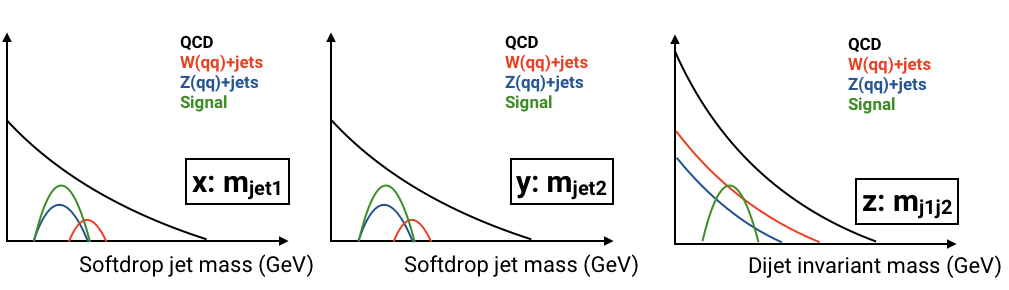
\includegraphics[width=0.99\textwidth]{figures/analysis/search3/misc/3Dfit.png}
\caption{An illustration of the shape of the signal and the relative background contributions in the three relevant dimensions $\MJO$(x), $\MJT$(y) and $\MVV$(z). }
\label{fig:searchIII:3Dfit}
\end{figure}
\begin{itemize}
  \item \textbf{Signal 3D PDF:} Resonant in x, y and z. Parametrized as function of the resonance mass \mX
  \item \textbf{Non-resonant background:} Non-resonant in x, y and z and dominant background. Created through a foorward folding kernel approach
  \item \textbf{Resonant background:} Mainly W/Z+jets (some \ttbar). Resonant in x and y, smoothly falling in z.
  \item \textbf{Alternative shapes:} 5 additional shape uncertainties implemented through vertical morphing  
\end{itemize}
These are illustrated in Figure~\ref{fig:searchIII:3Dfit} and will be described in detail in the following.

\subsection{Modeling of the signal}
The signal shape in three dimensions is defined as a product of the shape of the resonance mass and the jet masses:
\begin{equation}
	\footnotesize
	P_{sig}(\MVV,\MJO,\MJT|\theta(M_X) ) = P_{VV}(\MVV|\theta_1(M_X)) \times P_{j1}(\MJO|\theta_2(M_X))\\ \times P_{j2}(\MJT|\theta_2(M_X)).
\end{equation} 
The shapes for \MVV, \MJO and \MJT all depend on the hypothesized mass of the new particle ($M_X$) and a set of parameters $\theta=(\theta_1, \theta_2)$ that in principle depend on $M_X$.
The signal is parametrized by fitting the resonance mass and jet mass line shapes for each mass point, extracting the fitted parameters and then interpolating these as a function of the resonance mass
hypothesis. 
For the resonance mass \MVV, the sum of a crystal-ball function and a Gaussian shape is used for each mass point, following the shapes used in Search II.
Figure~\ref{fig:MVVShapeParam} shows the derived parameters and interpolation as a function of resonance mass.
The final \MVV shapes as extracted from the parametrization are shown in Figure~\ref{fig:MVVfromjson}.

\begin{figure}[htpb]
\centering
\resizebox{0.4\textwidth}{!}{\includegraphics*{figures/analysis/search3/AN-17-303/signalFits/Signal_mVV_MEAN.pdf}}
\resizebox{0.4\textwidth}{!}{\includegraphics*{figures/analysis/search3/AN-17-303/signalFits/Signal_mVV_SIGMA.pdf}}\\
\resizebox{0.4\textwidth}{!}{\includegraphics*{figures/analysis/search3/AN-17-303/signalFits/Signal_mVV_ALPHA1.pdf}}
\resizebox{0.4\textwidth}{!}{\includegraphics*{figures/analysis/search3/AN-17-303/signalFits/Signal_mVV_ALPHA2.pdf}}\\
\resizebox{0.4\textwidth}{!}{\includegraphics*{figures/analysis/search3/AN-17-303/signalFits/Signal_mVV_N1.pdf}}
\resizebox{0.4\textwidth}{!}{\includegraphics*{figures/analysis/search3/AN-17-303/signalFits/Signal_mVV_N2.pdf}}
\caption{The interpolated Crystal-ball parameters for the dijet invariant mass as a function of $M_X$. The small variations for ALPHA2 have been shown to have no effect on the overall modeling.}
\label{fig:MVVShapeParam}
\end{figure}


\begin{figure}[htpb]
\centering
\resizebox{0.6\textwidth}{!}{\includegraphics*{figures/analysis/search3/AN-17-303/signalFits/signalShapes_mVV_All.pdf}}
\caption{Final $\MVV$ signal shapes extracted from the parametrization. Here for a $\BulkG$ decaying to WW (blue) and ZZ (red) and for a $\Wpr$ decaying to WZ (green).}
\label{fig:MVVfromjson}
\end{figure}
The same procedure is used to model the jet mass: The \MJO spectrum for each resonance mass hypothesis is fitted using a double Crystal-ball function, the fitted parameters are extracted and interpolated as functions of the resonance mass. 
This is done separately for $\MJO$ and $\MJT$. The fitted parameters and interpolations are shown in Figure~\ref{fig:MJet1ShapeParam} for \MJO, the corresponding distributions for \MJT are in Appendix~\ref{app:search3:sigfits}.
\begin{figure}[htpb]
\centering
\resizebox{0.4\textwidth}{!}{\includegraphics*{figures/analysis/search3/AN-17-303/signalFits_2016/Signal_mjetl1_mean.pdf}}
\resizebox{0.4\textwidth}{!}{\includegraphics*{figures/analysis/search3/AN-17-303/signalFits_2016/Signal_mjetl1_sigma.pdf}}\\
\resizebox{0.4\textwidth}{!}{\includegraphics*{figures/analysis/search3/AN-17-303/signalFits_2016/Signal_mjetl1_alpha.pdf}}
\resizebox{0.4\textwidth}{!}{\includegraphics*{figures/analysis/search3/AN-17-303/signalFits_2016/Signal_mjetl1_alpha2.pdf}}\\
\resizebox{0.4\textwidth}{!}{\includegraphics*{figures/analysis/search3/AN-17-303/signalFits_2016/Signal_mjetl1_n.pdf}}
\resizebox{0.4\textwidth}{!}{\includegraphics*{figures/analysis/search3/AN-17-303/signalFits_2016/Signal_mjetl1_n2.pdf}}
\caption{The interpolated double Crystal-ball parameters for the softdrop jet mass as a function of $M_X$. To improve the stability of the fit some parameters are set constant. Here for jet 1.}
\label{fig:MJet1ShapeParam}
\end{figure}
The final \MJO shapes as extracted from the parametrization are shown in Figures~\ref{fig:MJfromjson}.
\begin{figure}[htpb]
\centering
\resizebox{0.6\textwidth}{!}{\includegraphics*{figures/analysis/search3/AN-17-303/signalFits/signalShapes_mJ_All.pdf}}
\caption{Final $\MJ$ signal shapes extracted from the parametrization for a $\BulkG$ decaying to ZZ, a $\BulkG$ decaying to WW and for a $\Wpr$ decaying to WZ.}
\label{fig:MJfromjson}
\end{figure}
Finally, the signal yield is parametrized as a function of the resonance mass. For each mass point $M_X$ and each purity category, the signal yield per picobarn of cross section is calculated as the integral of the Monte Carlo histogram.
The yields are then interpolated as a function of $M_X$. The signal efficiency as a function of resonance mass is shown in Figure~\ref{fig:SignalYields}.
\begin{figure}[htpb]
\centering
\resizebox{0.6\textwidth}{!}{\includegraphics*{figures/analysis/search3/AN-17-303/signalFits_2016/signalEff.pdf}}
\caption{Signal efficiency as a function of resonance mass.}
\label{fig:SignalYields}
\end{figure}



\subsection{Modeling of the non-resonant background}
\label{sec:nonresbkgd}

In order to model the QCD multijets background in the three-dimensional \MVV-\MJO-\MJT plane, we use the following conditional product:
\begin{equation}
	\footnotesize
	P(\MVV,\MJO,\MJT) = P_{VV}(\MVV|\theta_1) \times P_{cond,1}(\MJO|\MVV,\theta_2) \times P_{cond,2}(\MJT|\MVV,\theta_2).
\end{equation} 
This probability density requires a computation of the conditional two-dimensional shapes of $\MJO/\MJT$ given $\MVV$, as well as a one dimensional shape of the $\MVV$ distribution.

The following fit range and binning is used for the three axes: \MJO/\MJT is fitted from 55 to 215 GeV using 2 GeV bins. $\MVV$ is fitted from 1126 to 5500 GeV. The lower bound is chosen such that to avoid complications in the fitting procedure due to trigger turn-on effects, while the upper bound is chosen considering the highest dijet invariant mass found in data as well as avoiding mis-reconstruction effects at very large $m_{jj}$ and low jet masses. For $\MVV$, the "dijet binning" is used. This binning corresponds to the actual dijet mass resolution and is, in units of \GeV:\newline


Dijet binning = 1126, 1181, 1246, 1313, 1383, 1455, 1530, 1607, 1687, 1770, 1856, 1945, \\
2037, 2132, 2231, 2332, 2438, 2546, 2659, 2775, 2895, 3019, 3147, 3279, 3416, 3558, 3704, \\
3854, 4010, 4171, 4337, 4509, 4686, 4869, 5058, 5253, 5500\newline


The background model is built starting from simulation and we encode sufficient nuisance parameters into the fit, allowing the shape
to adapt itself to data. For this we use a "forward-folding" approach. For each MC event in the two(one)-dimensional \MVV-\MJ(\MJ) space, a 2D(1D) Gaussian kernel is built starting from generator level quantities. Each of these Gaussians then contribute to the total probability density of the final two(one)-dimensional probability density functions

First, the resonance mass and softdrop jet mass scale and resolution are derived. 
For this we use the anti-$k_T$ generated jet collection matched to jets identified as V-jets on reconstruction level.
We then derived the $\MJ$ and $\MVV$ scale and resolution from a Gaussian fit to $M_{i}(\mathrm{reco})/M_{i}(\mathrm{gen})$ ($i=\MJ$ or $i=\MVV$ ) in bins of generator jet $\PT$.
Figure~\ref{fig:resoFits} shows the fit to $M_{jet}(\mathrm{reco})/M_{jet}(\mathrm{gen})$ (left) and $M_{jj}(\mathrm{reco})/M_{jj}(\mathrm{gen})$ (right) for an arbitrary bin. The Gaussian mean yields the mass scale and the Gaussian width the mass resolution.
\begin{figure}[h!]
\centering
\resizebox{0.4\textwidth}{!}{\includegraphics*{figures/analysis/search3/AN-17-303/detRes/detectorResolution/debug_fit_mjres_8.png}}
\resizebox{0.4\textwidth}{!}{\includegraphics*{figures/analysis/search3/AN-17-303/detRes/detectorResolution/debug_fit_mvvres_8.png}}\\
\caption{ Fit to $M_{jet}(\mathrm{reco})/M_{jet}(\mathrm{gen})$ (left) and $M_{jj}(\mathrm{reco})/M_{jj}(\mathrm{gen})$. 
The mass resolution is taken as the width of the fitted Gaussian, while the Gaussian mean yields the mass scale.}
\label{fig:resoFits}
\end{figure}
The resonance mass and softdrop jet mass scale and resolution as a function of generator jet $\PT$ is shown in Figure~\ref{fig:ScaleResolution}.
\begin{figure}[h!]
\centering
\resizebox{0.4\textwidth}{!}{\includegraphics*{figures/analysis/search3/AN-17-303/detRes/detectorresolution_resxHisto.png}}
\resizebox{0.4\textwidth}{!}{\includegraphics*{figures/analysis/search3/AN-17-303/detRes/detectorresolution_resyHisto.png}}\\
\resizebox{0.4\textwidth}{!}{\includegraphics*{figures/analysis/search3/AN-17-303/detRes/detectorresolution_scalexHisto.png}}
\resizebox{0.4\textwidth}{!}{\includegraphics*{figures/analysis/search3/AN-17-303/detRes/detectorresolution_scaleyHisto.png}}
\caption{Resolution (top) and scale (bottom) for $\MVV$ (left) and the $\MJ$ (right) as a function of generator jet $\PT$.}
\label{fig:ScaleResolution}
\end{figure}
The projection of these resolution functions are shown in Figure~\ref{fig:ResolutionProfiles}.
\begin{figure}[h!]
\centering
\resizebox{0.4\textwidth}{!}{\includegraphics*{figures/analysis/search3/AN-17-303/detRes/detectorresolution_mvv.png}}
\resizebox{0.4\textwidth}{!}{\includegraphics*{figures/analysis/search3/AN-17-303/detRes/detectorresolution_mjet.png}}\\
\caption{Projections of the resolution functions for all generator jet $\PT$ bins for $\MVV$ (left) and $\MJ$ (right).}
\label{fig:ResolutionProfiles}
\end{figure}
The mass scale and resolution are then used to populate the conditional 2D histogram as follows. Each generated event is smeared with a 2D Gaussian kernel 
\begin{equation}
k(\MJ,\MVV) =\frac{w_i}{\sqrt{2\pi}r_{\MVV,i}\cdot r_{\MJ,i}} \exp \left (-\frac{1}{2} \left ( \frac{\MVV-s_{\MVV,i}}{r_{\MVV,i}} \right)^2 -\frac{1}{2} \left ( \frac{\MJ-s_{\MJ,i}}{r_{\MJ,i}} \right)^2 \right ),   
\end{equation}
where $s_{i}, r_{i}$ are the scale and the resolution derived in the previous step and $w_i$ is the event weight product (e.g PU, cross sections etc.). 
The resulting kernel values are filled into a 2D histogram. This procedure is performed separately for \MJO and \MJT. To build the one-dimensional template for the dijet invariant mass the same procedure as above is used, with the exception that
the smearing is done with one-dimensional Gaussian kernel only depending on $\MVV$.
The templates are then added together to form a three-dimensional PDF. Finally, we fit this 3D PDF to QCD MC in order to remove any residual bias (mainly at the extreme ends of the spectra). The result is a full, smooth shape replacing the prediction from simulation.\par
As the HPHP category is very limited in statistics, we rather build this template starting from the HPLP templates. This is done by fitting the HPLP 3D PDF to QCD MC in the HPHP category. Figure~\ref{fig:3DkernelsHPLPpythia} show the final templates (solid lines) together with the QCD MC (data points) derived from the 2017 MC in the HPLP (top) and HPHP category (bottom). Good agreement between QCD MC and templates in all three dimensions is observed, within statistical uncertainties. The corresponding distributions in 2016 MC can be found in Appendix~\ref{app:search3:2016kernels}.\par
\begin{figure}[h!]
\centering
\resizebox{0.3\textwidth}{!}{\includegraphics*{figures/analysis/search3/AN-17-303/backgroundFits/3Dkernels_HPLP_pythia_2017/cx.png}}
\resizebox{0.3\textwidth}{!}{\includegraphics*{figures/analysis/search3/AN-17-303/backgroundFits/3Dkernels_HPLP_pythia_2017/cy.png}}
\resizebox{0.3\textwidth}{!}{\includegraphics*{figures/analysis/search3/AN-17-303/backgroundFits/3Dkernels_HPLP_pythia_2017/cz.png}}\\
\resizebox{0.3\textwidth}{!}{\includegraphics*{figures/analysis/search3/AN-17-303/backgroundFits/3Dkernels_HPHP_pythia_2017/cx.png}}
\resizebox{0.3\textwidth}{!}{\includegraphics*{figures/analysis/search3/AN-17-303/backgroundFits/3Dkernels_HPHP_pythia_2017/cy.png}}
\resizebox{0.3\textwidth}{!}{\includegraphics*{figures/analysis/search3/AN-17-303/backgroundFits/3Dkernels_HPHP_pythia_2017/cz.png}}
\caption{Comparison between QCD MC simulation (markers) and kernels derived from generator level quantities (lines) for the HPHP (top) and HPLP (bottom) categories using 2017 MC. The kernels are shown for \MJO (left), \MJT (middle) and \MVV (right).}
\label{fig:3DkernelsHPHPpythia}
\end{figure}
In order to validate the kernel transfer method, we check that we can fit a higher-statistics HPHP region by loosening the $\tau_{21}^{DDT}$ cut to 0.49. This results in 12 times more background events in the HPHP category, and should uncover whether any degeneracy is present in the fits themselves and whether HPLP indeed is capable of modeling HPHP, without being camouflaged by large error bars. The resulting kernel versus MC spectra are shown in Figure~\ref{fig:looseDDT_closure}. Good closure is observed in all three dimensions, demonstrating that the HPLP kernels adapt well to the HPHP MC data points even when statistics are sufficient, and we consider the method sound.
\begin{figure}[h!]
\centering
\resizebox{0.3\textwidth}{!}{\includegraphics*{figures/analysis/search3/AN-17-303/backgroundFits/looseDDT_HPHP/cx.png}}
\resizebox{0.3\textwidth}{!}{\includegraphics*{figures/analysis/search3/AN-17-303/backgroundFits/looseDDT_HPHP/cy.png}}
\resizebox{0.3\textwidth}{!}{\includegraphics*{figures/analysis/search3/AN-17-303/backgroundFits/looseDDT_HPHP/cz.png}}
\caption{Comparison between QCD MC simulation (markers) and kernels derived from generator level quantities (lines) in the HPHP category, using a looser cut on $\tau_{21}^{DDT}$.}
\label{fig:looseDDT_closure}
\end{figure}
\clearpage

\subsection{Modeling of the resonant background}
\label{sec:resbkgd}
In addition to the QCD multijet background, there are a few sub-dominant processes to consider which contain one real vector boson and at least one QCD-jet. These are W+jets, Z+jets and events from \ttbar processes. They are resonant around the W/Z mass in the two softdrop jet mass dimensions and must threfore be treated differently than the non-resonant QCD background. Figure \ref{fig:stack_res_bkg} shows the projections on \MJO (left), \MJT (middle) and \MVV (right).
\begin{figure}[h!]
 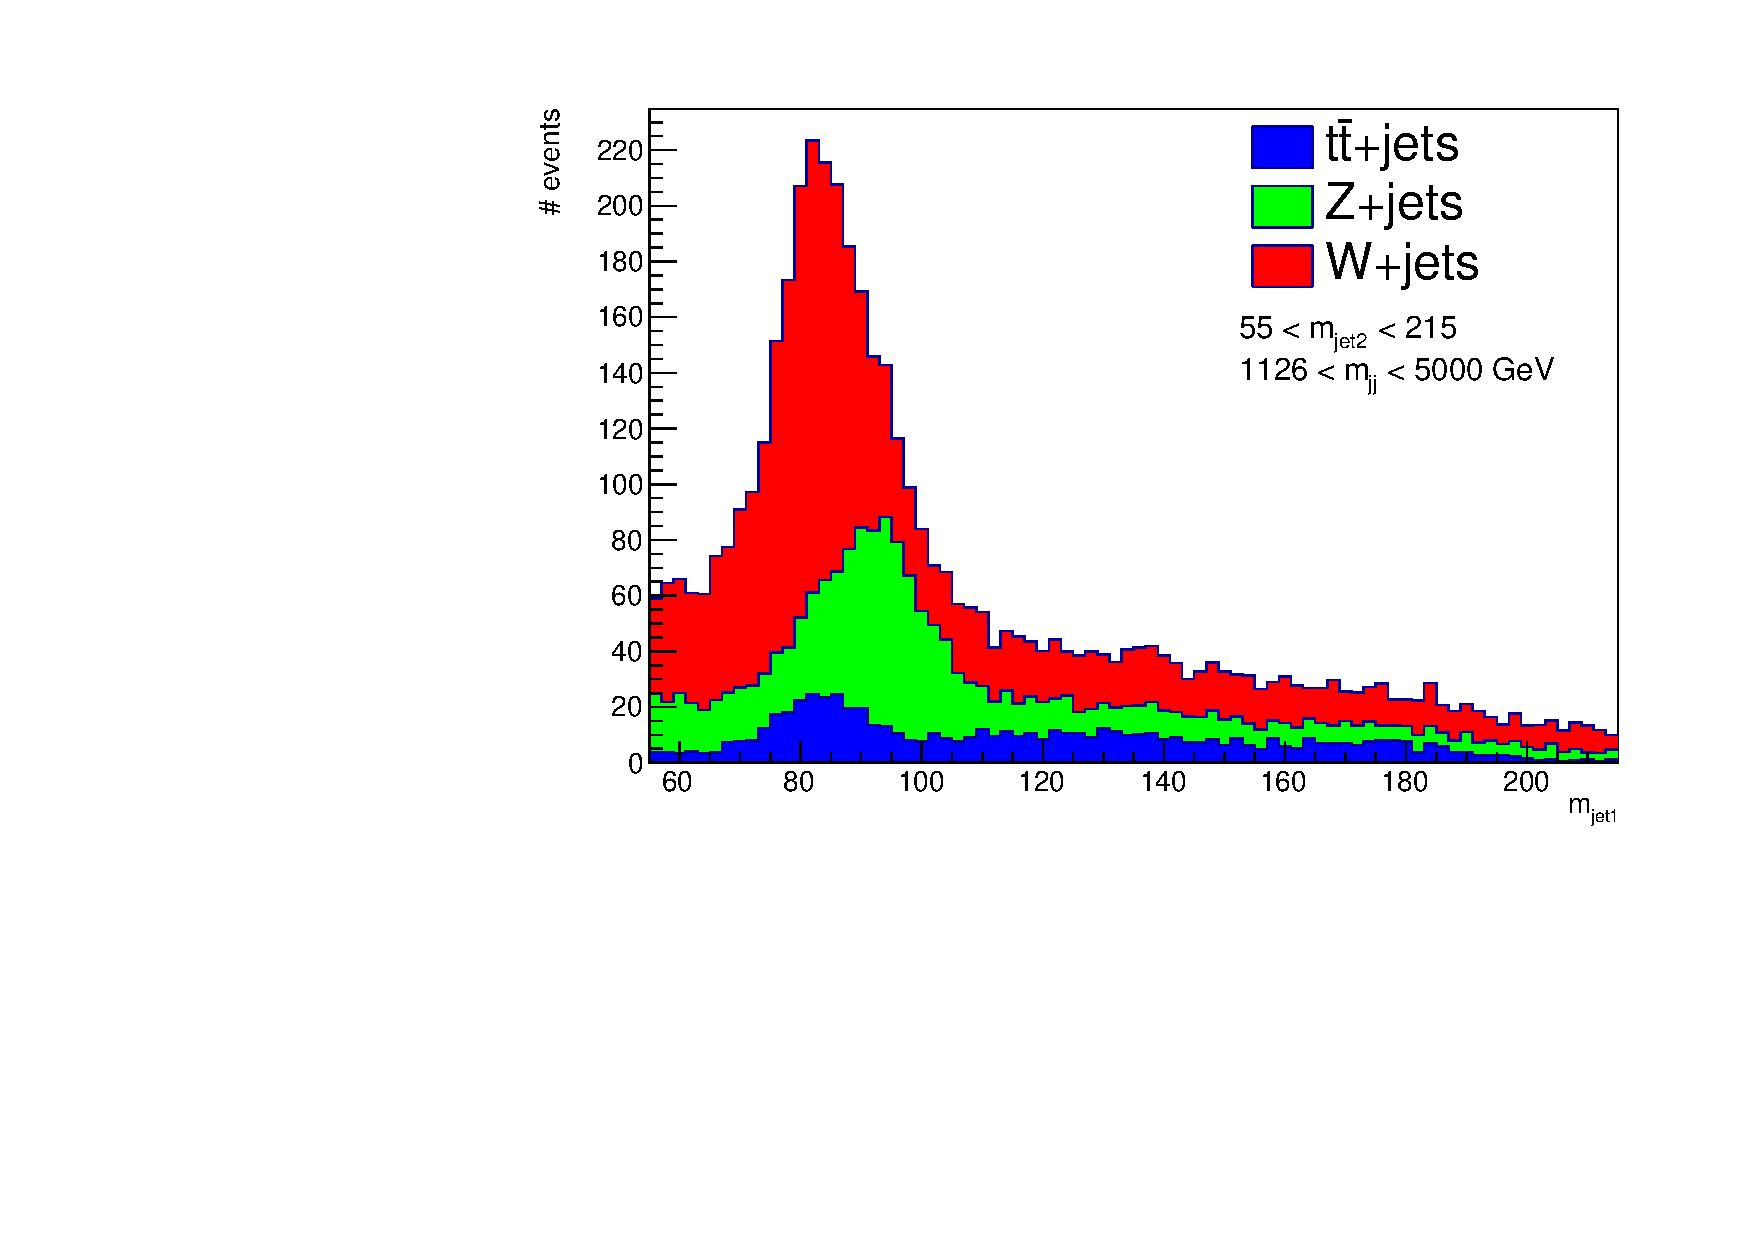
\includegraphics[width=0.329\textwidth]{figures/analysis/search3/AN-17-303/resonantBkg/CP_background_px_xrange55-215_yrange55-215zrange1126-5000_HPLP.pdf}
 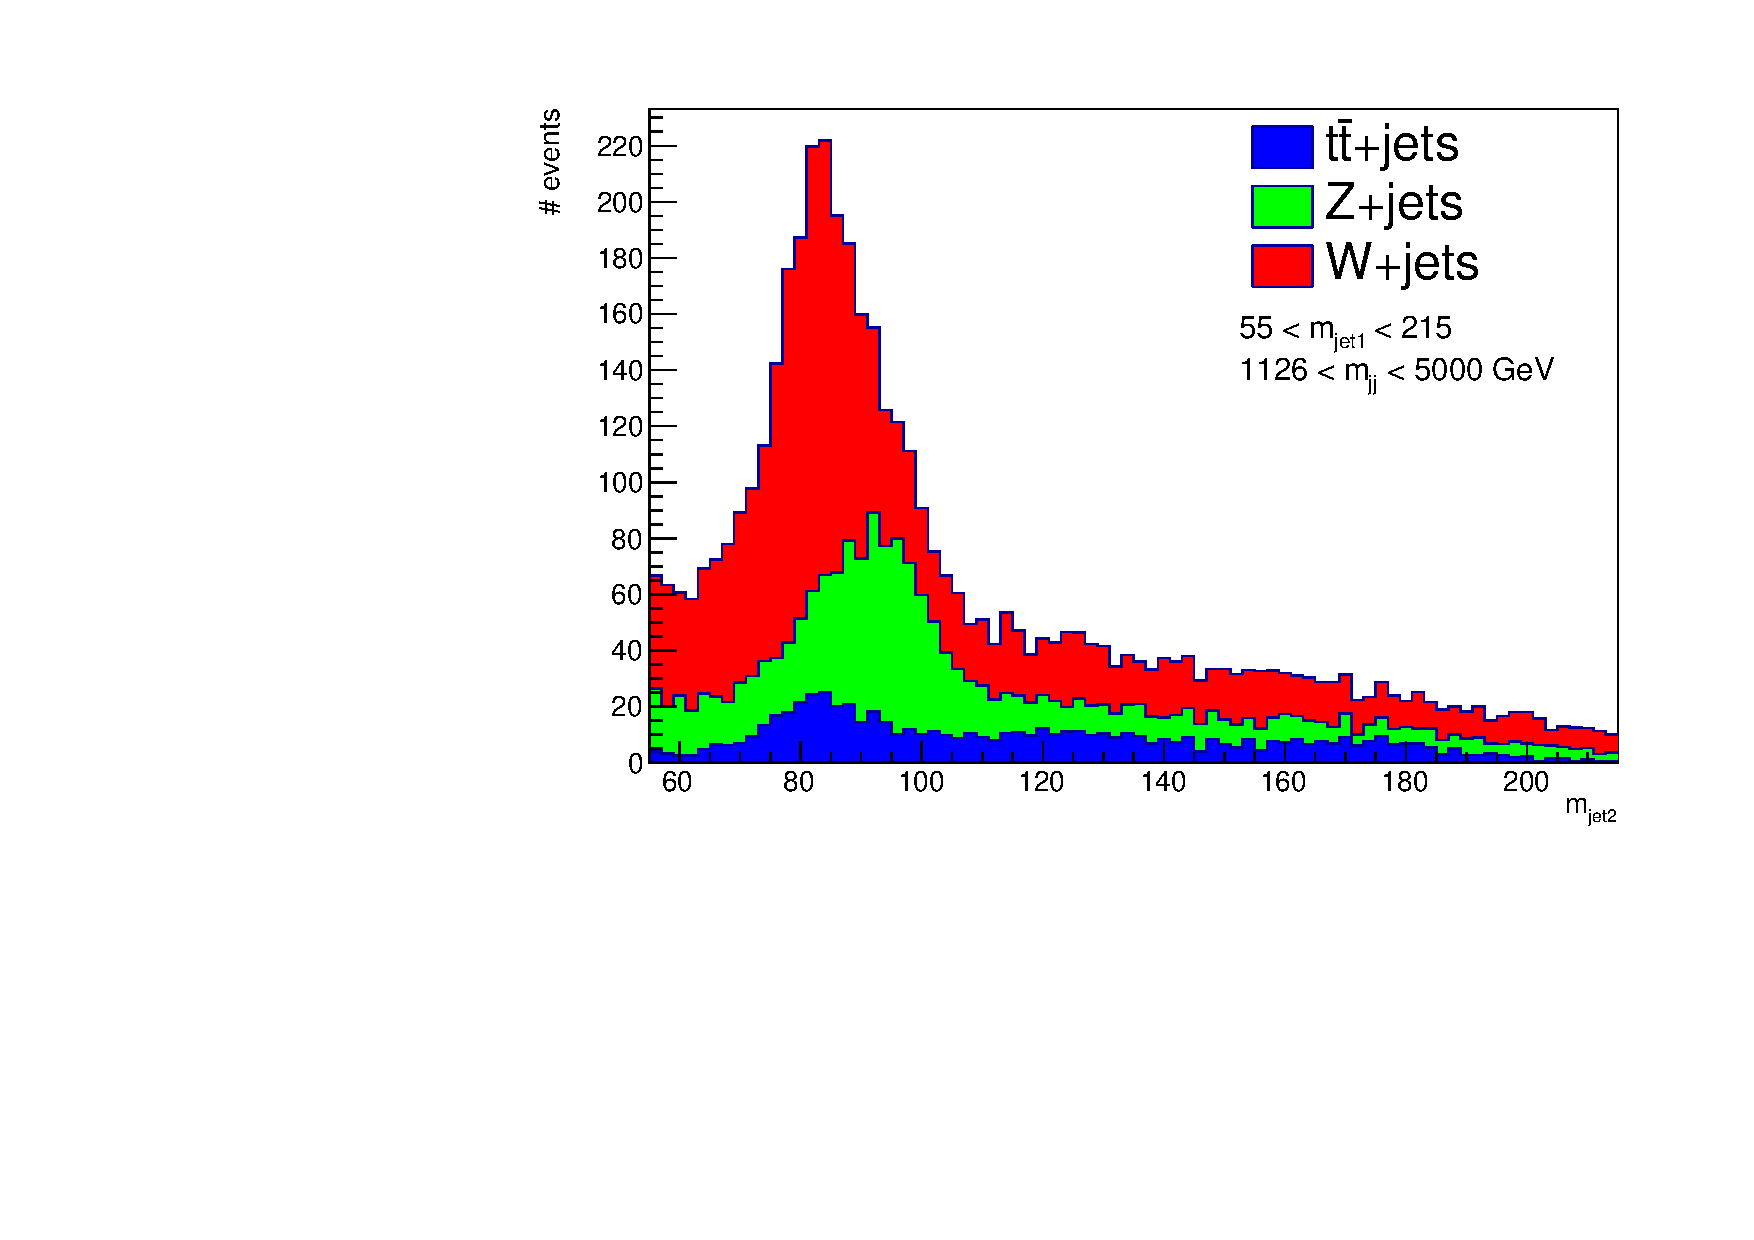
\includegraphics[width=0.329\textwidth]{figures/analysis/search3/AN-17-303/resonantBkg/CP_background_py_xrange55-215_yrange55-215zrange1126-5000_HPLP.pdf}
 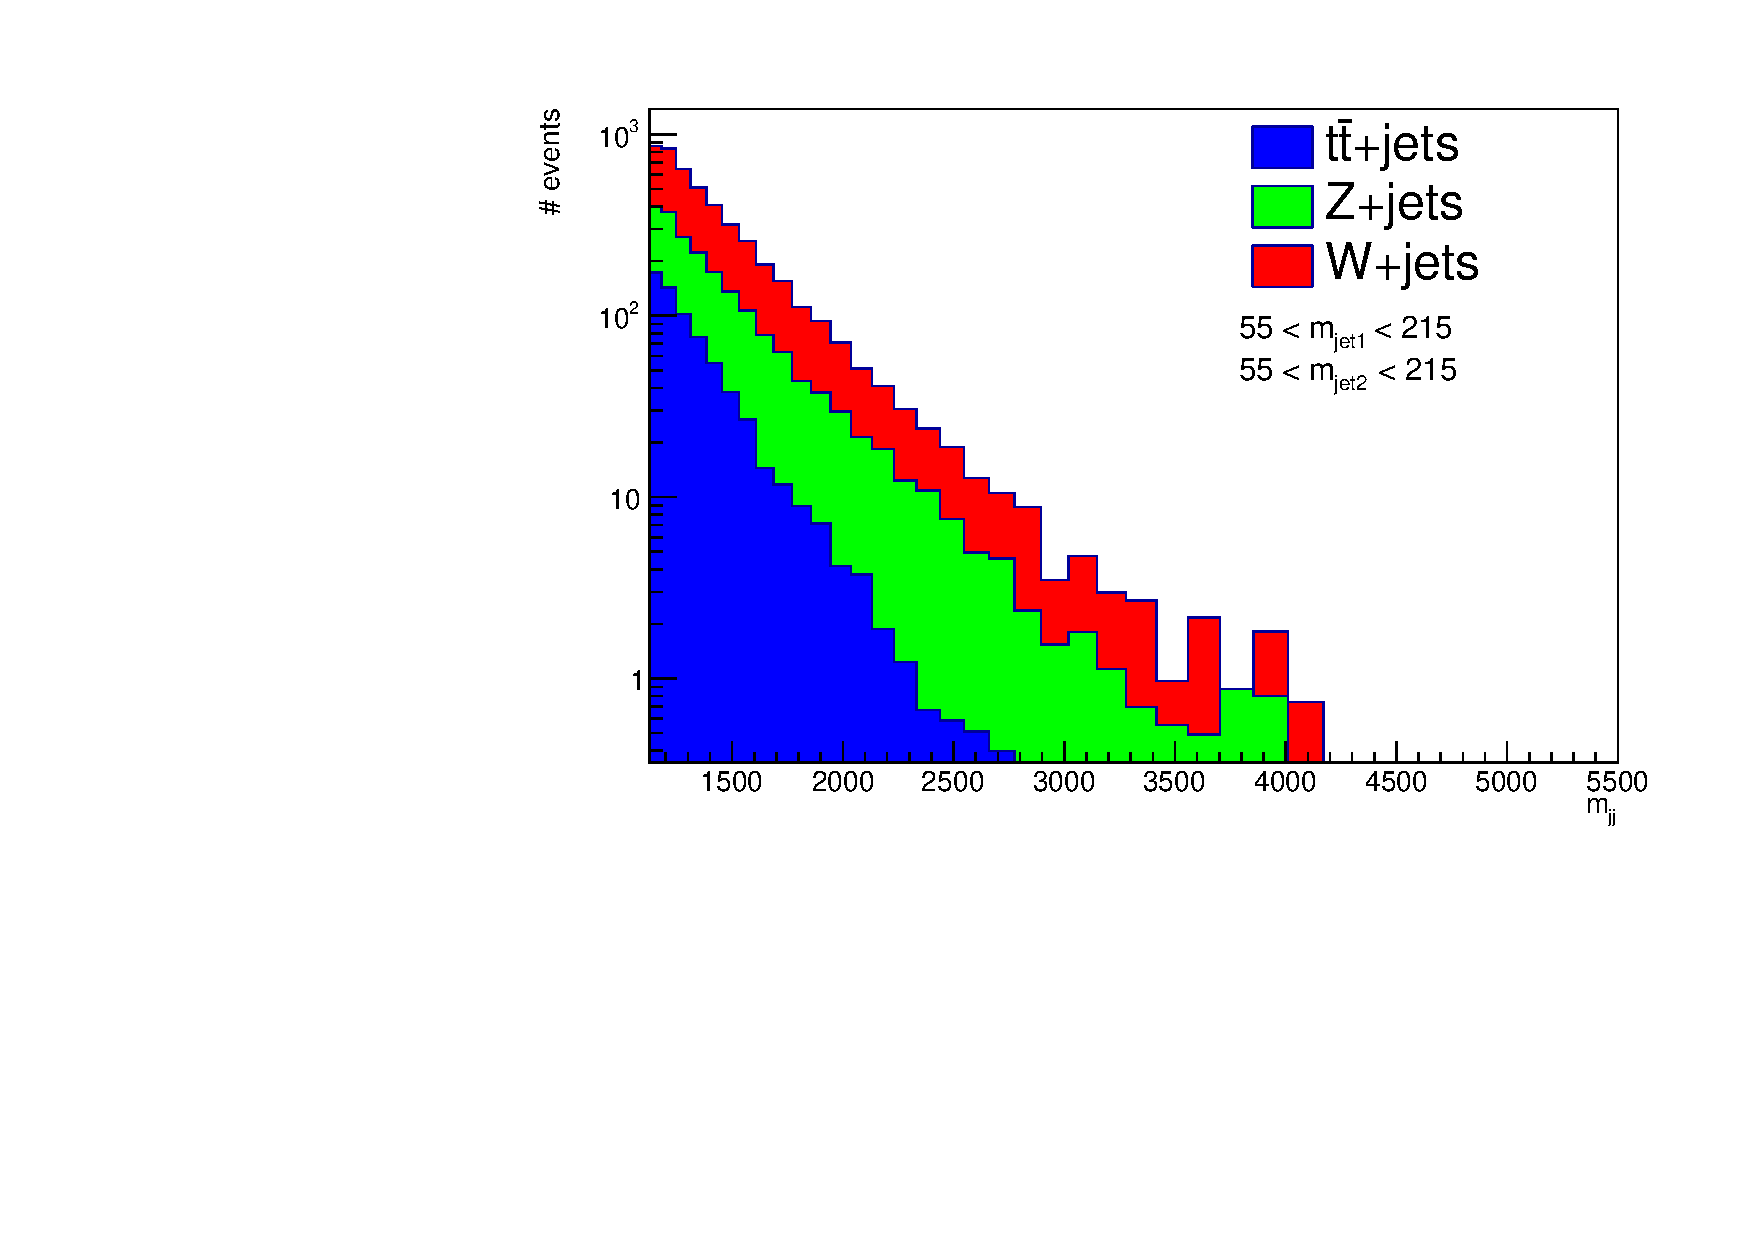
\includegraphics[width=0.329\textwidth]{figures/analysis/search3/AN-17-303/resonantBkg/CP_background_pz_xrange55-215_yrange55-215zrange1126-5000_HPLP.pdf}
\caption{Projections of the sub-dominant backgrounds on the jet mass axes \MJO (left) and \MJT (middle), as well as on the dijet invariant mass \MVV (right). Here in the low purity category.}
\label{fig:stack_res_bkg}
\end{figure}
As the jets are randomly sorted, each jet mass dimension contains two contributions: A resonant part consisting of real vector boson jets, peaking around the V mass, and a non-resonant part composed of jets originating from a quark or a gluon, similar to the QCD multijets background. These two contributions are modeled separately as we know that the non-resonant part of the jet mass spectrum is correlated with the dijet invariant mass (like QCD), while the resonant part is not. We additionally want to encode the fact that we know these backgrounds in reality only peaks in one jet mass axis (there is only one real vector boson) by requiring the PDFs to consist of a resonant part on one axis, and a non-resonant part on the other axis. A three dimensional PDF for the sub-dominant backgrounds is built as a product of three one dimensional pdf's as follows:
\begin{align}
	\label{eq:searchIII:vjetpdf}
	P_{res} \left(\MJO, \MJT, \MVV \right) &= P_{VV} \left( \MVV \right) \times  P_{jet1} \left( \MJO, \MJT \right) \times P_{jet2} \left( \MJT, \MJO \right)
\end{align}
where
\begin{align}
P_{jet1} \left( \MJO, \MJT \right) &= f \times R(\MJT) \times P_{res} ( \MJO ) + (1-f) P_{non-res} (\MJO ) \\
P_{jet2} \left( \MJT, \MJO \right) &= (1-f) \times R(\MJO) \times P_{res} ( \MJT ) + f P_{non-res} (\MJT )
\end{align}
Here, $R(\MJ)$ parametrizes the correlation between \MJO and \MJT and $f$ is a fit parameter that is used to adjust the fraction of real vector boson jets in
\MJO compared to \MJT. It's value can vary 10\% around $f=0.5$, the expected median when using a random jet sorting.\newline
As the contribution of the t$\bar{\text{t}}$ background is much smaller than the one coming from V+jets (less than 2\%), it is modeled together with the W+jets contribution. Therefore only two PDFs are built for the resonant background: One for the W+jets and t$\bar{\text{t}}$, and one for Z+jets.\newline
The available MC statistics in the high purity category is very low and therefore the parametrization of the resonant background is done for the low purity category only, and the resulting shapes are then used for both purity categories. The uncertainties for the different purity categories are, however, included as separate nuisance parameters in the fit.\par
The non-resonant \MVV PDF is constructed using the same kernel approach as is used to model the QCD multijet background with one minor difference: Due to the low statistics in the high-\MVV tail, an additional smoothing of the jet mass tail using a leveled exponential
\begin{equation}
\frac{\text{d} N}{\text{d} m_{jj}} = \frac{P_0 (1-m_{jj}/s)^{P_1}}{(m_{jj}/s)^{P_2}}
\end{equation}
is performed. Here, $s$ is the center of mass energy. The function is fitted to the spectrum starting from a dijet mass of 1.1 (2.1)~TeV for high purity (low purity). Two uncertainties on this shape is added in order to accommodate for MC mis-modelig due to higher order QCD and electroweak corrections: One proportional to \MVV and one proportional to 1/\MVV. The resulting \MVV kernels (solid lines) for the W+jets background are shown in Figure \ref{fig:Vjets_mvv} and are compared to MC simulation (markers). The blue line corresponds to the nominal shape, while the red and green lines correspond to the uncertainties proportional to \MVV and 1/\MVV, respectively. The corresponding distributions for the Z+jets background are shown in Appendix~\ref{app:search3:resbkg}.\par
\begin{figure}[h]
\centering
\resizebox{0.49\textwidth}{!}{\includegraphics*{figures/analysis/search3/AN-17-303/resonantBkg/debug_mVV_kernels_WJets_HPHP.png}}
\resizebox{0.49\textwidth}{!}{\includegraphics*{figures/analysis/search3/AN-17-303/resonantBkg/debug_mVV_kernels_WJets_HPLP.png}}\\
% \resizebox{0.49\textwidth}{!}{\includegraphics*{figures/analysis/search3/AN-17-303/resonantBkg/debug_mVV_kernels_ZJets_HPHP.pdf}}
% \resizebox{0.49\textwidth}{!}{\includegraphics*{figures/analysis/search3/AN-17-303/resonantBkg/debug_mVV_kernels_ZJets_HPLP.pdf}}
\caption{One dimensional \MVV kernels (solid line) compared to MC (markers) for the W+jets background in the HPHP (left) and HPLP (right) categories. The blue line corresponds to the nominal shape, while the red and green lines correspond to uncertainties proportional to \MVV and 1/\MVV, respectively.}
\label{fig:Vjets_mvv}
\end{figure}
As mentioned above, the modeling of the \MJ spectrum is split into two different PDFs: One describing the resonant and one describing the non-resonant part. We distinguish between the two by requiring the resonant contribution to consist of jets matched to a generated boson within a cone of $\Delta R = 0.8$. A double-sided crystal-ball function is then fitted to the resonant spectrum for W+jets and Z+jets separately. This allows us to fully correlate uncertainties on the mean and width of the \MJ distribution for signal with the corresponding values for W/Z+jets, as these uncertainties affect all jets generated from real vector bosons in the same way. This effectively gives us a way of constraining these parameters directly from data. The parametrization of the resonant part of the jet mass spectrum for \MJO is shown in Figure \ref{fig:Vjets_fits} for W+jets and \ttbar (left) and Z+jets. The small enhancement around 170 \GeV is caused by fully merged top jets and is so small ($<2\%$ in the low purity and $<0.5\%$ in the high purity category) that we do not take it into account in the final PDF.
\begin{figure}[h!]
\centering
\resizebox{0.45\textwidth}{!}{\includegraphics*{figures/analysis/search3/AN-17-303/resonantBkg/debugJl1_Wjets_TTbar_Res.png}}
\resizebox{0.45\textwidth}{!}{\includegraphics*{figures/analysis/search3/AN-17-303/resonantBkg/debugJl1_Zjets_Res.png}}
\caption{Fit to the resonant part of the V+jets and \ttbar spectrum for W+jets and \ttbar (left) and Z+jets (right).}
\label{fig:Vjets_fits}
\end{figure}
The non-resonant part of the V+jets background is modeled using a simple Gaussian fit to the spectrum of jets not matched to a real vector bosons, as shown in Figure \ref{fig:Vjets_fits_nonRes}.
\begin{figure}[h!]
\centering
\resizebox{0.49\textwidth}{!}{\includegraphics*{figures/analysis/search3/AN-17-303/resonantBkg/debugJl1_Wjets_TTbar_nonRes.png}}
\resizebox{0.49\textwidth}{!}{\includegraphics*{figures/analysis/search3/AN-17-303/resonantBkg/debugJl1_Zjets_nonRes.png}}
\caption{Fit to the non-resonant part of the V+jets and \ttbar spectrum for W+jets and \ttbar (left) and Z+jets (right).}
\label{fig:Vjets_fits_nonRes}
\end{figure}
For the resonant modeling, correlations between the jet mass \MJ and dijet invariant mass \MVV have been found small enough to be neglected (the jet mass spectrum does not, within statistical uncertainties, depend on the jet \PT). However, there is a strong correlation between the softdrop jet mass of each jet due to the fact that when one of the two jets originates from a real boson peaking around the V mass, the other is bound to be a quark jet. Therefore, the fraction of real boson jets contained in \MJO affects the fraction of real V jets in \MJT. To account for this, the fraction of real V jets versus quark/gluon jets jets, is parametrized as a function of the jet mass. As the jets are randomly sorted, we define the parametrization as
\begin{align}
R(\MJ) &= \frac{N_{res,jet1}(\MJT)+N_{res,jet2}(\MJO)}{N_{non-res,jet1}(\MJT) + N_{non-res,jet2}(\MJO)}~.
\end{align}
Where $N(\MJ)$ denotes the number of events within a given \MJ window. The resulting ratio is then fitted with a polynomial function, as shown in Figure~\ref{fig:ratio_Vjets}.
\begin{figure}[h]
\centering
\resizebox{0.45\textwidth}{!}{\includegraphics*{figures/analysis/search3/AN-17-303/resonantBkg/debug_corr_l1_l2_Wjets.pdf}}
\resizebox{0.45\textwidth}{!}{\includegraphics*{figures/analysis/search3/AN-17-303/resonantBkg/debug_corr_l1_l2_Zjets.pdf}}
\caption{Ratio of resonant to non-resonant events in  W+jets (left) and Z+jets (right) as a function of jet mass.}
\label{fig:ratio_Vjets}
\end{figure}
As a closure test, the three dimensional kernel as defined in Equation~\ref{eq:searchIII:vjetpdf} is fitted to the V+jets and \ttbar simulation. Figure~\ref{fig:searchIII:Vjets_closure} shows the fitted kernel (red) together with the MC data points (black markers) in the low (top) and high (bottom) purity categories. Mostly good agreement is observed along all dimensions, with some deviations in the very high \MVV tail in the high purity category. This is, however, a region dominated with very little statistics and is completely swallowed up by the QCD multijets background which has the same shape.
\begin{figure}[h!]
\centering
\resizebox{0.32\textwidth}{!}{\includegraphics*{{figures/analysis/search3/AN-17-303/resonantBkg/PostFitVjetsMC_X-Proj._y_:_0,-1_z_:_0,-1}.png}}
\resizebox{0.32\textwidth}{!}{\includegraphics*{{figures/analysis/search3/AN-17-303/resonantBkg/PostFitVjetsMC_Y-Proj._x_:_0,-1_z_:_0,-1}.png}}
\resizebox{0.32\textwidth}{!}{\includegraphics*{{figures/analysis/search3/AN-17-303/resonantBkg/PostFitVjetsMC_Z-Proj._x_:_0,-1_y_:_0,-1}.png}}\\
\resizebox{0.32\textwidth}{!}{\includegraphics*{{figures/analysis/search3/AN-17-303/resonantBkg/PostFitVjetsMC_HPHP_X-Proj._y_:_0,-1_z_:_0,-1}.png}}
\resizebox{0.32\textwidth}{!}{\includegraphics*{{figures/analysis/search3/AN-17-303/resonantBkg/PostFitVjetsMC_HPHP_Y-Proj._x_:_0,-1_z_:_0,-1}.png}}
\resizebox{0.32\textwidth}{!}{\includegraphics*{{figures/analysis/search3/AN-17-303/resonantBkg/PostFitVjetsMC_HPHP_Z-Proj._x_:_0,-1_y_:_0,-1}.png}}
\caption{Final fits of the complete background model (red line) to the MC simulation of the V+jets backgrounds (black markers) for the high purity category.}
\label{fig:searchIII:Vjets_closure}
\end{figure}
\clearpage

\subsection{Systematic uncertainties}
\label{sec:searchIII:sysunc}

Systematic uncertainties are inserted as nuisance parameters in the fit and affect the normalization and shape of both signal and background.

\subsubsection{Signal normalization uncertainties}
As all background contributions are data driven, the largest systematic uncertainties affect only the signal.
\begin{itemize}
\item {\bf luminosity } 2.6\%(2.3\%) for the 2016(2017) dataset
\item {\bf $\tau_{21}^{DDT}$ efficiency } 1-12\% systematic uncertainty on the signal efficiency scale factor for the $\tau_{21}^{DDT}$ selection (listed in Table~\ref{tab:wsf_total}). Anti-correlated between the HP and LP categories.
\item {\bf $\tau_{21}^{DDT}$ \PT{} extrapolation } An additional uncertainty arising from the extrapolation of the V-tagging efficiency scale factors towards higher transverse momenta. Treated as correlated between the $\tau_{21}^{DDT}$ categories and is given as $3.9\% \times \ln(p_T/200~\GeV)$ and $8.5\% \times \ln(p_T/200~\GeV)$ for the LP and HP regions, respectively. 
\item {\bf PDF and factorization/renormalization scale } 2\% uncertainty on the signal acceptance due to choice of PDFs and factorization/renormalization scale. 
\end{itemize} 


\subsubsection{Background normalization uncertainties}
The QCD multijet background has a poorly known cross section and is therefore allowed to float within 50\% of the yield expected by simulation. For the resonant V+jets background, the following uncertainties on the normalization is added: One due to cross section ($\sim5\%$), one due to NLO QCD corrections ($\sim10\%$) and one due NLO electroweak corrections ($\sim15-35\%$).

\subsubsection{Signal and resonant background shape uncertainties}
There are two shape uncertainties correlated between the signal and V+jets background: Systematics due to jet mass scale (JMS) and jet mass resolution (JMR). These are evaluated in a \ttbar control region, listed in Table~\ref{tab:wsf_total}, and affect the mean and width of the jet mass PDFs. 
Three additional shape uncertainties are added for the signal: Uncertainties due to jet energy scale (JES), jet energy resolution (JER) and PDF. The uncertainty due to JES/JER is evaluated by reweighting the transverse momentum of each MC event in signal MC, then fitting a Gaussian to the dijet invariant mass spectrum and calculating the change in the mean and variance with respect to no reweighting. These are then used as uncertainties on the signal \MVV shape (2\% for the dijet mass scale, 5\% for the resolution).\newline
Uncertainties due to the PDF are evaluated by reweighting each event according to $\approx$~100 PDF variations. The impact on the signal shapes are again evaluated by fitting a Gaussian to the $m_{jet}$ and $m_{jj}$ distributions before and after changing PDF weights. The obtained variation is $<1\%$ for the 2017 signal MC, but slightly higher in 2016. An overall uncertainty on the acceptance of 3\% is therefore applied. 


\subsubsection{Non-resonant background shape uncertianties}
Alternate shapes for the non-resonant background components are added to the fit through vertical template morphing. This creates nuisance parameters for each additional shape shape, allowing the derived nominal 3D PDF to vary within the respective nuisances to match the data. Shape uncertainties that simultaneously affect all three dimensions are used, totaling to 5 to take all possible effects into account. The first effect accounts for variation of the underlying transverse momentum spectrum and is obtained through an alternate shape produced by varying the jet masses \MJ and dijet mass \MVV by a quantity proportional to \MVV and \MJ. The second effect considered is a variation of the scale, where the corresponding alternate shape is obtained by simultaneously varying \MJ and \MVV up and down by a quantity proportional to 1/\MVV and 1/\MJ.
Finally, as we do no know a priori whether Nature behaves more like \PYTHIA{8}, \HERWIG{++} or \MADGRAPH{}+\PYTHIA{8}, we account for differences due to MC generation and parton shower modeling by adding three additional shapes corresponding to the PDFs obtained using different QCD MC generators.\newline
Those five shape uncertainties are assigned very large pre-fit values (allowed to float within 33\%), effectively allowing the simulation to take any value to describe the data. The alternate shapes described above are shown in Figure~\ref{fig:searchIII:sys}, here for the 2017 analysis.

\begin{figure}[h!]
\centering
\resizebox{0.3\textwidth}{!}{\includegraphics*{figures/analysis/search3/AN-17-303/backgroundFits/3Dkernels_HPHP_pythia_2017/cxSyst.png}}
\resizebox{0.3\textwidth}{!}{\includegraphics*{figures/analysis/search3/AN-17-303/backgroundFits/3Dkernels_HPHP_pythia_2017/cySyst.png}}
\resizebox{0.3\textwidth}{!}{\includegraphics*{figures/analysis/search3/AN-17-303/backgroundFits/3Dkernels_HPHP_pythia_2017/czSyst.png}}\\
\resizebox{0.3\textwidth}{!}{\includegraphics*{figures/analysis/search3/AN-17-303/backgroundFits/3Dkernels_HPLP_pythia_2017/cxSyst.png}}
\resizebox{0.3\textwidth}{!}{\includegraphics*{figures/analysis/search3/AN-17-303/backgroundFits/3Dkernels_HPLP_pythia_2017/cySyst.png}}
\resizebox{0.3\textwidth}{!}{\includegraphics*{figures/analysis/search3/AN-17-303/backgroundFits/3Dkernels_HPLP_pythia_2017/czSyst.png}}
\caption{The nominal MC data (markers) and smooth nominal kernel obtained from \PYTHIA{8} (black line), together with the five alternate shapes added to the fit as shape nuisance parameters. Here for the high (top) and low (bottom) categories.}
\label{fig:searchIII:sys}
\end{figure}
\clearpage

\subsection{Results}
The distributions obtained from a combined fit to the observed data in 2016 and 2017 are shown in Fig.~\ref{fig:searchIII:finalPostFit}, with the corresponding predicted and observed number of background events in the signal region summarized in Table~\ref{tab:searchIII:ObsEvents}.
\begin{table}[b]

\centering
\begin{tabular}{lcc} 
 & HPHP & HPLP\\
 \hline
 \hline
W+jets & 113.3 $\pm$ 18.1 & 4257.4 $\pm$ 257.0 \\
            & 100.4 (exp.) & 4318.0 (exp.)\\
Z+jets & 46.5 $\pm$ 8.3 & 1747.5 $\pm$ 163.7\\
           & 50.2 (exp.) & 2159.0 (exp.) \\
QCD  & 651.6 $\pm$ 4.0 & 51190.5 $\pm$ 313.1 \\
          & 684.4 (exp.) & 53767.5 (exp.) \\
\hline
Observed yield & 778 $\pm$ 28 & 57227 $\pm$ 239\\
Post-fit total background & 811.4 $\pm$ 20.3 & 57195.5 $\pm$ 436.8\\
\hline
\hline

\end{tabular} 
\caption{Expected and observed yields and their total uncertainty (stat.+sys.) in the two purity categories.} 
\label{tab:searchIII:ObsEvents}
\end{table}

\begin{figure}[h!]
\centering
\resizebox{0.32\textwidth}{!}{\includegraphics*{figures/analysis/search3/AN-17-303/postfitchecks/postfit_HPHP_unblind/PostFitComboHPHP_X-Proj__y___0_-1_z___0_-1.png}}
\resizebox{0.32\textwidth}{!}{\includegraphics*{figures/analysis/search3/AN-17-303/postfitchecks/postfit_HPHP_unblind/PostFitComboHPHP_Y-Proj__x___0_-1_z___0_-1.png}}
\resizebox{0.32\textwidth}{!}{\includegraphics*{figures/analysis/search3/AN-17-303/postfitchecks/postfit_HPHP_unblind/PostFitComboHPHP_Z-Proj__x___0_-1_y___0_-1.png}}\\
\resizebox{0.32\textwidth}{!}{\includegraphics*{figures/analysis/search3/AN-17-303/postfitchecks/postfit_HPLP_unblind/PostFitComboHPLP_X-Proj__y___0_-1_z___0_-1.png}}
\resizebox{0.32\textwidth}{!}{\includegraphics*{figures/analysis/search3/AN-17-303/postfitchecks/postfit_HPLP_unblind/PostFitComboHPLP_Y-Proj__x___0_-1_z___0_-1.png}}
\resizebox{0.32\textwidth}{!}{\includegraphics*{figures/analysis/search3/AN-17-303/postfitchecks/postfit_HPLP_unblind/PostFitComboHPLP_Z-Proj__x___0_-1_y___0_-1.png}}
\caption{Postfit distribution after a fit to 2016 and 2017 data projected onto the \MJO (left), \MJT (middle), and \MVV (right) axis. Here for the HPHP (top) and HPLP (bottom) category. The background shape uncertainty is shown as a red shaded band,  and the statistical uncertainties of the data are shown as vertical bars. The overlaid signal distribution is arbitrarily normalized.}
\label{fig:searchIII:finalPostFit}
\end{figure}
\subsubsection{Limits}
As for Search I and Search II, exclusion limits on the cross section of the process $\text{X} \to VV$ are set in the context of the Bulk Graviton model and the HVT model~B scenario (again obtained using the asymptotic $\text{CL}_\text{S}$ method). Figure~\ref{fig:searchIII:limitsCombo} show the resulting expected and observed 95\% confidence level exclusion limits on the signal cross section as a function of the resonance mass for all signal models. The obtained limits are compared with the resonance production cross section times the branching fraction to $\PW\PW$, $\PZ\PZ$ and $\PW\PZ$.
\begin{figure}[h!]
\centering
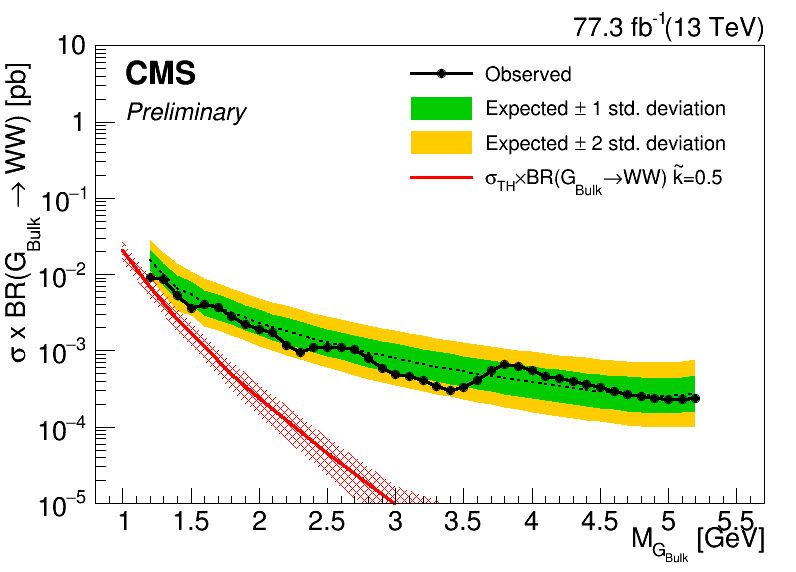
\includegraphics[width=0.45\textwidth]{figures/analysis/search3/AN-17-303/limits/limits_BulkGWW_combo_2016_2017.png}
\includegraphics[width=0.45\textwidth]{figures/analysis/search3/AN-17-303/limits/limits_BulkGZZ_combo_2016_2017.png}\\
\includegraphics[width=0.45\textwidth]{figures/analysis/search3/AN-17-303/limits/limits_WprimeWZ_combo_2016_2017.png}
\includegraphics[width=0.45\textwidth]{figures/analysis/search3/AN-17-303/limits/limits_ZprimeWW_combo_2016_2017.png}
\caption{Expected limits obtained combining 35.9\fbinv and 41.4\fbinv of data of data after combining all purity categories for Bulk $G\rightarrow WW$ (top left), Bulk $G\rightarrow ZZ$ 
(top right), $\PWpr\rightarrow WZ$ (bottom left) and $\PZpr\rightarrow WW$ (bottom right) signals.}
\label{fig:searchIII:limitsCombo}
\end{figure}
To settle the question of whether the 3D fit method yields an improvement upon the 1D search method, we compare the limits obtained above to those obtained using the 1D fit method (the results from SearchII). In Figure~\ref{fig:limitsCompare} we see a 20--30\% improvement for all signal hypothesis with the new method (comparing the 1D and 3D 2016 limits only), and a total gain of about 35---40\% when combining the 2016 and 2017 datasets.
\begin{figure}[h!]
\centering
\includegraphics[width=0.45\textwidth]{figures/analysis/search3/AN-17-303/limits/limits_BulkGWW_compare.png}
\includegraphics[width=0.45\textwidth]{figures/analysis/search3/AN-17-303/limits/limits_BulkGZZ_compare.png}\\
\includegraphics[width=0.45\textwidth]{figures/analysis/search3/AN-17-303/limits/limits_WprimeWZ_compare.png}
\includegraphics[width=0.45\textwidth]{figures/analysis/search3/AN-17-303/limits/limits_ZprimeWW_compare.png}
\caption{CA comparison of the 3D expected limits split into dataset (2016 and 2017), to that obtained with the 1D fit using 2016 data. Here for $\BulkG\rightarrow WW$ (top left), $\BulkG\rightarrow ZZ$ (top right), $\PWpr\rightarrow WZ$ (bottom left) and $\PZpr\rightarrow WW$ (bottom right) signals.}
\label{fig:limitsCompare}
\end{figure}
In Figure~\ref{fig:limitsCompareATLAS}, we additionally compare the 3D limits to those obtained by the ATLAS collaboration in a similar search~\cite{ATLAS-CONF-2018-016} and find this search to be up to 35\% more sensitive for the two signal scenarios considered (the \BulkG limits can not be compared due to different values of $\tilde{k}$).
\begin{figure}[h!]
\centering
\includegraphics[width=0.45\textwidth]{figures/analysis/search3/AN-17-303/limits/limits_WprimeWZ_compare_ATLAS.png}
\includegraphics[width=0.45\textwidth]{figures/analysis/search3/AN-17-303/limits/limits_ZprimeWW_compare_ATLAS.png}
\caption{A comparison of the limits obtained above, to those by the ATLAS collaboration in a similar search~\cite{ATLAS-CONF-2018-016}. Here for \PWpr (left) and \PZpr (right) signal hypotheses.}
\label{fig:limitsCompareATLAS}
\end{figure}
Finally, in Figure~\ref{fig:limitsPerCat} we show a breakdown of the limits per purity category. As expected, the HPHP category dominates at low mass where background is high and the HPLP category dominates at high mass due to low background and high signal efficiency.
\begin{figure}[h!]
\centering
\includegraphics[width=0.45\textwidth]{figures/analysis/search3/AN-17-303/limits/limit_compare_BulkGWW_per_category.png}
\caption{Limits split into purity categories (HPHP and HPLP) for a Bulk $G\rightarrow WW$ signal hypothesis.}
\label{fig:limitsPerCat}
\end{figure}

\subsubsection{Pulls of nuisance parameters}
As summarized in Section~\ref{sec:searchIII:sysunc}, we add a list of systematic uncertainties to the fit as nuisance parameters.
To quantify how much the nuisances we insert differs from the ones preferred by the fit, we compute the pull
\begin{equation}
p_{\theta} = (\theta - \theta_{in})/\sigma_\theta
\end{equation}
where $\theta_{in}$ is the nuisance value pre-fit, $\theta$ the corresponding parameter post-fit and $\sigma_\theta$ its error.
and its error bar calculated as the ratio between post- and pre-fit uncertainty.
Figure~\ref{fig:searchIII:pullsCombo1617} shows the pulls for a signal+background fit to the combined (2016+2017) dataset (left) and when fitting the two separately (right), here using a signal hypothesis corresponding to a 2 \TeV \BulkG.
\begin{figure}[h!]
\centering
\includegraphics[width=0.45\textwidth]{figures/analysis/search3/AN-17-303/postfitchecks/pulls_Combo1617.png}
\includegraphics[width=0.45\textwidth]{figures/analysis/search3/AN-17-303/postfitchecks/pulls_16_vs_17.png}
\caption{Pulls of each nuisance parameter for a combined signal+background fit to the combined 2016+2017 dataset (left) and when fitting the two separately.}
\label{fig:searchIII:pullsCombo1617}
\end{figure}


\clearpage

\section{Outlook}
\label{sec:outlook}
In this chapter, we have followed the search for VV resonances in the all-hadronic final state through three stages: From being one of the first ever analysis in the ``boosted'' final state at 13 \TeV and the very first to take advantage of substructure at trigger level, through leading the development of a new W-tagging algorithm and mass corrections now default in CMS and finally ending with the development of a multi-dimensional fit for generic searches in jet groomed mass and dijet invariant mass.\par
Each analysis has built on significant improvements that came with the analysis before it: The substructure triggers and mass corrected softdrop jet mass are both used for the 3D fit, the early discovery of the softdrop signal efficiency dependence on \PT led us to derive corrections for it. Now the question which remains is: \emph{What comes next?}.\par
A few ideas were already mentioned in the introduction to Search III, Section~\ref{sec:searchIII}. The natural next step for this search, is an incorporation of the VH(bb) and H(bb)H(bb) final states into the three-dimensional fit. Orthogonality between the three would be done through b-tagging categories, as illust
